\documentclass{beamer}
\usetheme{Madrid}
\setbeamertemplate{bibliography item}{\insertbiblabel}

\usepackage[main=english,czech]{babel}
%\usepackage[T1]{fontenc}
\usepackage[utf8]{inputenc}
\usepackage{url}
\usepackage{caption}
\usepackage{graphicx}
\usepackage{xcolor}

\usepackage{appendixnumberbeamer}

\captionsetup[figure]{font=footnotesize, justification=justified, format=hang}

\usepackage{tikz}
\usepackage[warnundef]{jabbrv}
\usepackage[natbib,style=numeric-comp,sorting=none,backend=biber]{biblatex}
\addbibresource{bibliography.bib}

%%% Detailed settings of bibliography
\ifx\citet\undefined\else

% Maximum number of authors of a single work. If exceeded, "et al." is used.
\ExecuteBibliographyOptions{maxnames=2}
% The same setting specific to citations using \citet{...}
\ExecuteBibliographyOptions{maxcitenames=2}
% The same settings specific to the list of literature
%\ExecuteBibliographyOptions{maxbibnames=2}

% Shortening first names of authors: "E. A. Poe" instead of "Edgar Allan Poe"
%\ExecuteBibliographyOptions{giveninits}
% The same without dots ("EA Poe")
%\ExecuteBibliographyOptions{terseinits}

% If your bibliography entries are hard to break into lines, try this mode:
%\ExecuteBibliographyOptions{block=ragged}

% Possibly reverse the names of the authors with the non-ISO styles:
%\DeclareNameAlias{default}{family-given}

% Use caps-and-small-caps for family names in ISO 690 style.
\let\familynameformat=\textsc

% We want to separate multiple authors in citations by commas
% (while we use semicolons in the bibliography as per the ISO standard)
\DeclareDelimFormat[textcite]{multinamedelim}{\addcomma\space}
\DeclareDelimFormat[textcite]{finalnamedelim}{\space and~}

\fi

%%% Journal Abbreviations (jabbrv package) -- extra custom definitions (following ISO 4)
\DefineJournalPartialAbbreviation{Instrument}{Instrum}
\DefineJournalAbbreviation{Polonica}{Pol}
\DefineJournalPartialAbbreviation{Spectrometer}{Spectrom}

\AtBeginSection[]
{
	\begin{frame}<beamer>[noframenumbering]
		\frametitle{Outline}
		\tableofcontents[currentsection]
	\end{frame}
}

\title[OFTPC track simulation \& reconstruction]{Simulation and Reconstruction of $e^+$ and $e^-$ Trajectories in a Time Projection Chamber with Orthogonal Fields}
\subtitle{CZ+SK HEP Workshop 2026}
\author[M.~Vavřík]{\foreignlanguage{czech}{Martin Vavřík}\vspace{0.2cm}\\martin.vavrik@utef.cvut.cz\\IPNP CUNI \& IEAP CTU PRAGUE\\[0.2cm]
	\footnotesize Preprint: arXiv:2606.18821~\cite{vavřík2026}\vspace{-0.7cm}}
\logo{
\includegraphics[width=0.08\textwidth]{../images/mff_uk.png}}
\date{September 10, 2026}

\addtobeamertemplate{title page}{}{%
	\begin{tikzpicture}[remember picture, overlay]
		% Left logo (anchored to the west side of the page)
		\node[anchor=west] at ([xshift=0.7cm, yshift=-1.2cm]current page.west) {
			
\includegraphics[width=1.7cm]{../../figures/ieap_logo.jpg}
		};
		
		% Right logo (anchored to the east side of the page)
		\node[anchor=east] at ([xshift=-0.3cm, yshift=-1.2cm]current page.east) {
			
\includegraphics[width=2.7cm]{../../figures/drd1_logo.png}
		};
	\end{tikzpicture}
}

% Use for hiding the logo from some slides
\newcommand{\nologo}{\setbeamertemplate{logo}{}}
\newcommand{\nonav}{\setbeamertemplate{navigation symbols}{}}

\newcommand{\white}[1]{\textcolor{white}{#1}}
\renewcommand{\textapprox}{{\textasciitilde}}
\newcommand{\garfieldpp}{Garfield\texttt{++}}

\begin{document}
	
	\begin{frame}
		\titlepage
		\vspace{-0.9cm}
		\flushleft\scriptsize{Supervisor: Tomáš Sýkora, Consultant: Hugo Natal da Luz}\vspace{-0.15cm}
		\flushleft\scriptsize{Funding: GAČR GA21-21801S\\}
		\tiny{Computational resources were provided by the e-INFRA CZ project (ID:90254),\\ supported by the Ministry of Education, Youth and Sports of the Czech Republic.}
	\end{frame}
	
	\begin{frame}
		\frametitle{Outline}
		\tableofcontents
	\end{frame}
	
	\section{Motivation}
	{\nologo\nonav
	\begin{frame}
		\frametitle{Motivation: ATOMKI Measurements}
		\begin{itemize}
			\item Measurement of anomalies in the angular correlation of an~$e^+e^-$ pair internally produced in excited $ {}^8\text{Be} $~\cite{atomki_be,atomki_be2}, $ {}^4\text{He} $~\cite{atomki_he,atomki_he2} and $ {}^{12}\text{C} $~\cite{atomki_c}
			\item Angular resolution \textapprox7$^\circ$, energy resolution 4.5\% at 17.6 MeV
			\item Other experiments~\cite{dubna,hanoi,megii,padme}, but no independent measurement confirms or disproves it yet, possible explanation --- new boson X17~\cite{feng}
			\begin{columns}
				\column{0.33 \textwidth}
				\centering
				\vspace{0.1cm}
				\begin{minipage}[t][4cm]{\textwidth}
					\centering
					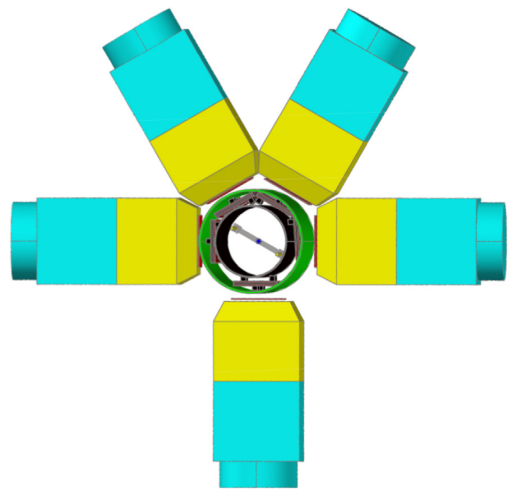
\includegraphics[width=0.9\textwidth]{../images/atomki_detector.png}
				\end{minipage}
				\small{ATOMKI spectrom.~\cite{atomki_det}}\\ \vspace{0.1cm}
				\tiny{Beam pipe (black), MWPC, $\Delta$E~det. (red), $E$~scintillators (yellow), light guides (blue)}
				\column{0.33 \textwidth}
				\centering
				\vspace{-0.2cm}
				\begin{minipage}[t][4cm]{\textwidth}
					\centering
					\includegraphics[width=\textwidth]{figures/atomki_be.png}
				\end{minipage}
				\footnotesize{$ {}^8\text{Be} $, $e^{+}e^{-}$ pair angular correlation.~\cite{atomki_be}}
				\column{0.28 \textwidth}
				\centering
				\vspace{-0.2cm}
				\begin{minipage}[t][4cm]{\textwidth}
					\centering
					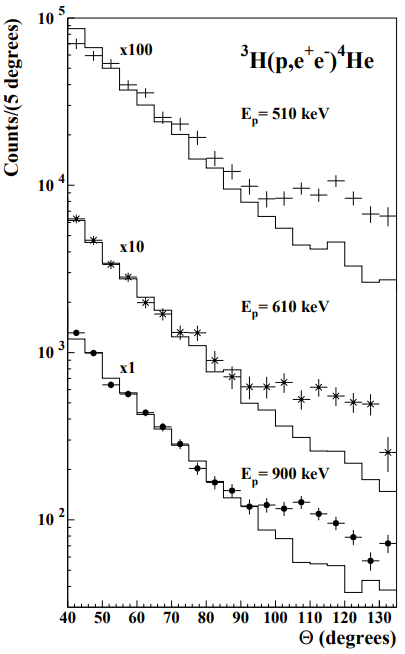
\includegraphics[width=0.7\textwidth]{../images/atomki_he.png}\newline
				\end{minipage}
				\footnotesize{$ {}^4\text{He} $, $e^{+}e^{-}$ pair angular correlation.~\cite{atomki_he}}
			\end{columns}
		\end{itemize}
	\end{frame}
	}
	
	\begin{frame}
		\frametitle{X17 Decay Signature in IPC}
		\centering
		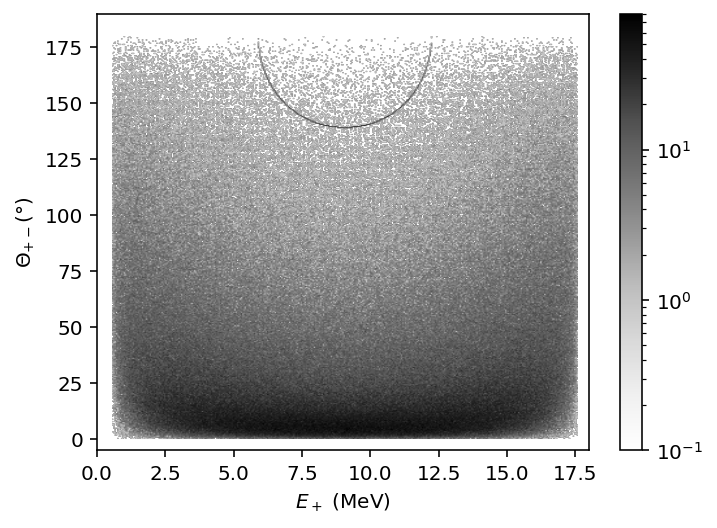
\includegraphics[width=0.75\textwidth]{../images/X17_sim.png}\\
		\vspace{-0.25cm}
		\begin{minipage}[t][4cm]{0.85\textwidth}
			\textbf{Geant 4 simulation (ideal case):} Histogram of e$^+$e$^-$ pair angle and positron energy produced by standard IPC and by the decay of a hypothetical boson X17 (branching ratio $3\cdot10^{-3}$).
		\end{minipage}
	\end{frame}
	
	{\nologo
	\begin{frame}
		\frametitle{OFTPC: Detector Configuration}
		\begin{itemize}
			\item Time Projection Chamber with Orthogonal Fields (OFTPC) -- electric and magnetic field perpendicular (gas mixture Ar/CO$_2$~--~70/30, \textcolor{gray}{\scriptsize 90/10})
			\item Reasons for OF: no solenoid, space constraints (SAMPA/SRS, number of channels)
		\end{itemize}
		\begin{columns}
			\column{0.48 \textwidth}
			\centering
			\begin{minipage}[t][4.05cm]{\textwidth}
				\centering
				\textcolor{white}{a\,\,}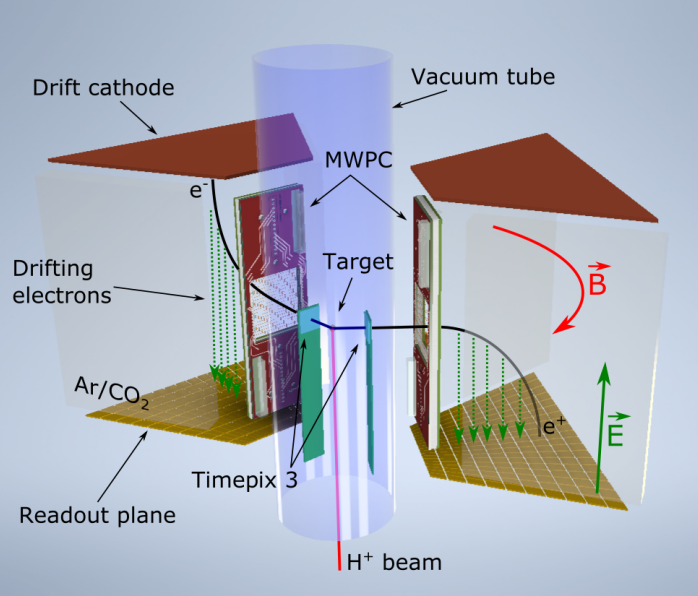
\includegraphics[width=0.9\linewidth]{../images/diagram.png}\newline
			\end{minipage}
			\small{Two out of the six OFTPC chambers.~\cite{x17_utef}}
			\column{0.02\textwidth}
			\column{0.48 \textwidth}
			\centering
			\begin{minipage}[t][4.05cm]{\textwidth}
				\centering
				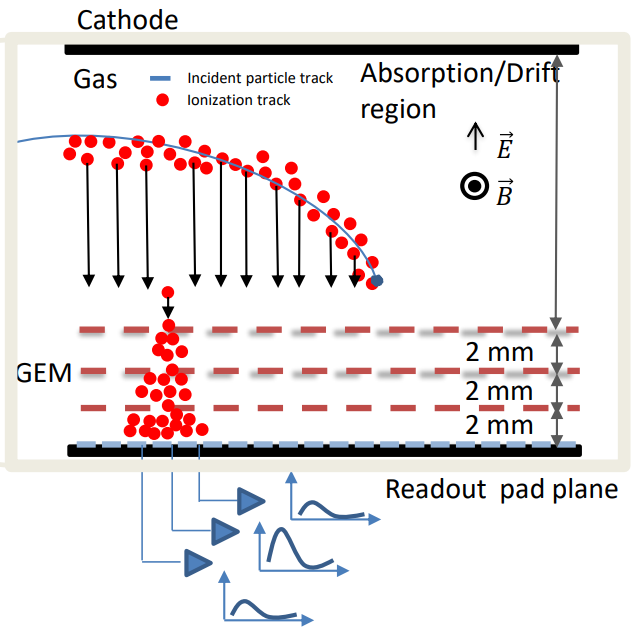
\includegraphics[width=0.8\linewidth]{../images/diagram2.png}\newline
			\end{minipage}
			\small{OFTPC with a triple gas electron multiplier (GEM) readout.~\cite{x17_utef}}
		\end{columns}
	\end{frame}
	
	\begin{frame}
		\frametitle{OFTPC: Detector Configuration}
		\centering
		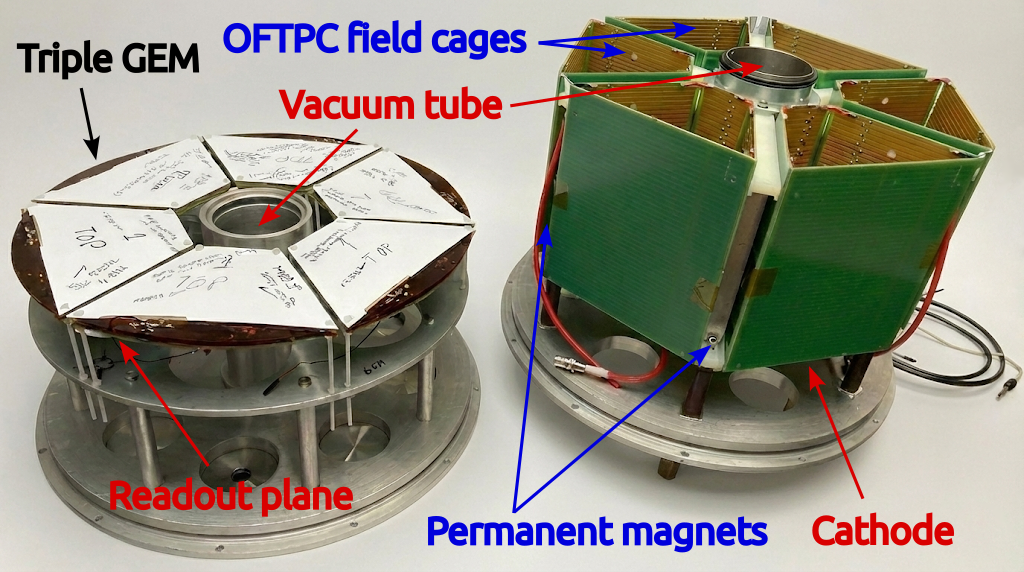
\includegraphics[width=\textwidth]{../../figures/X17_detector_labeled.png}
	\end{frame}
	
	\begin{frame}
		\frametitle{OFTPC: GEM Readout --- Pads}
		\centering
		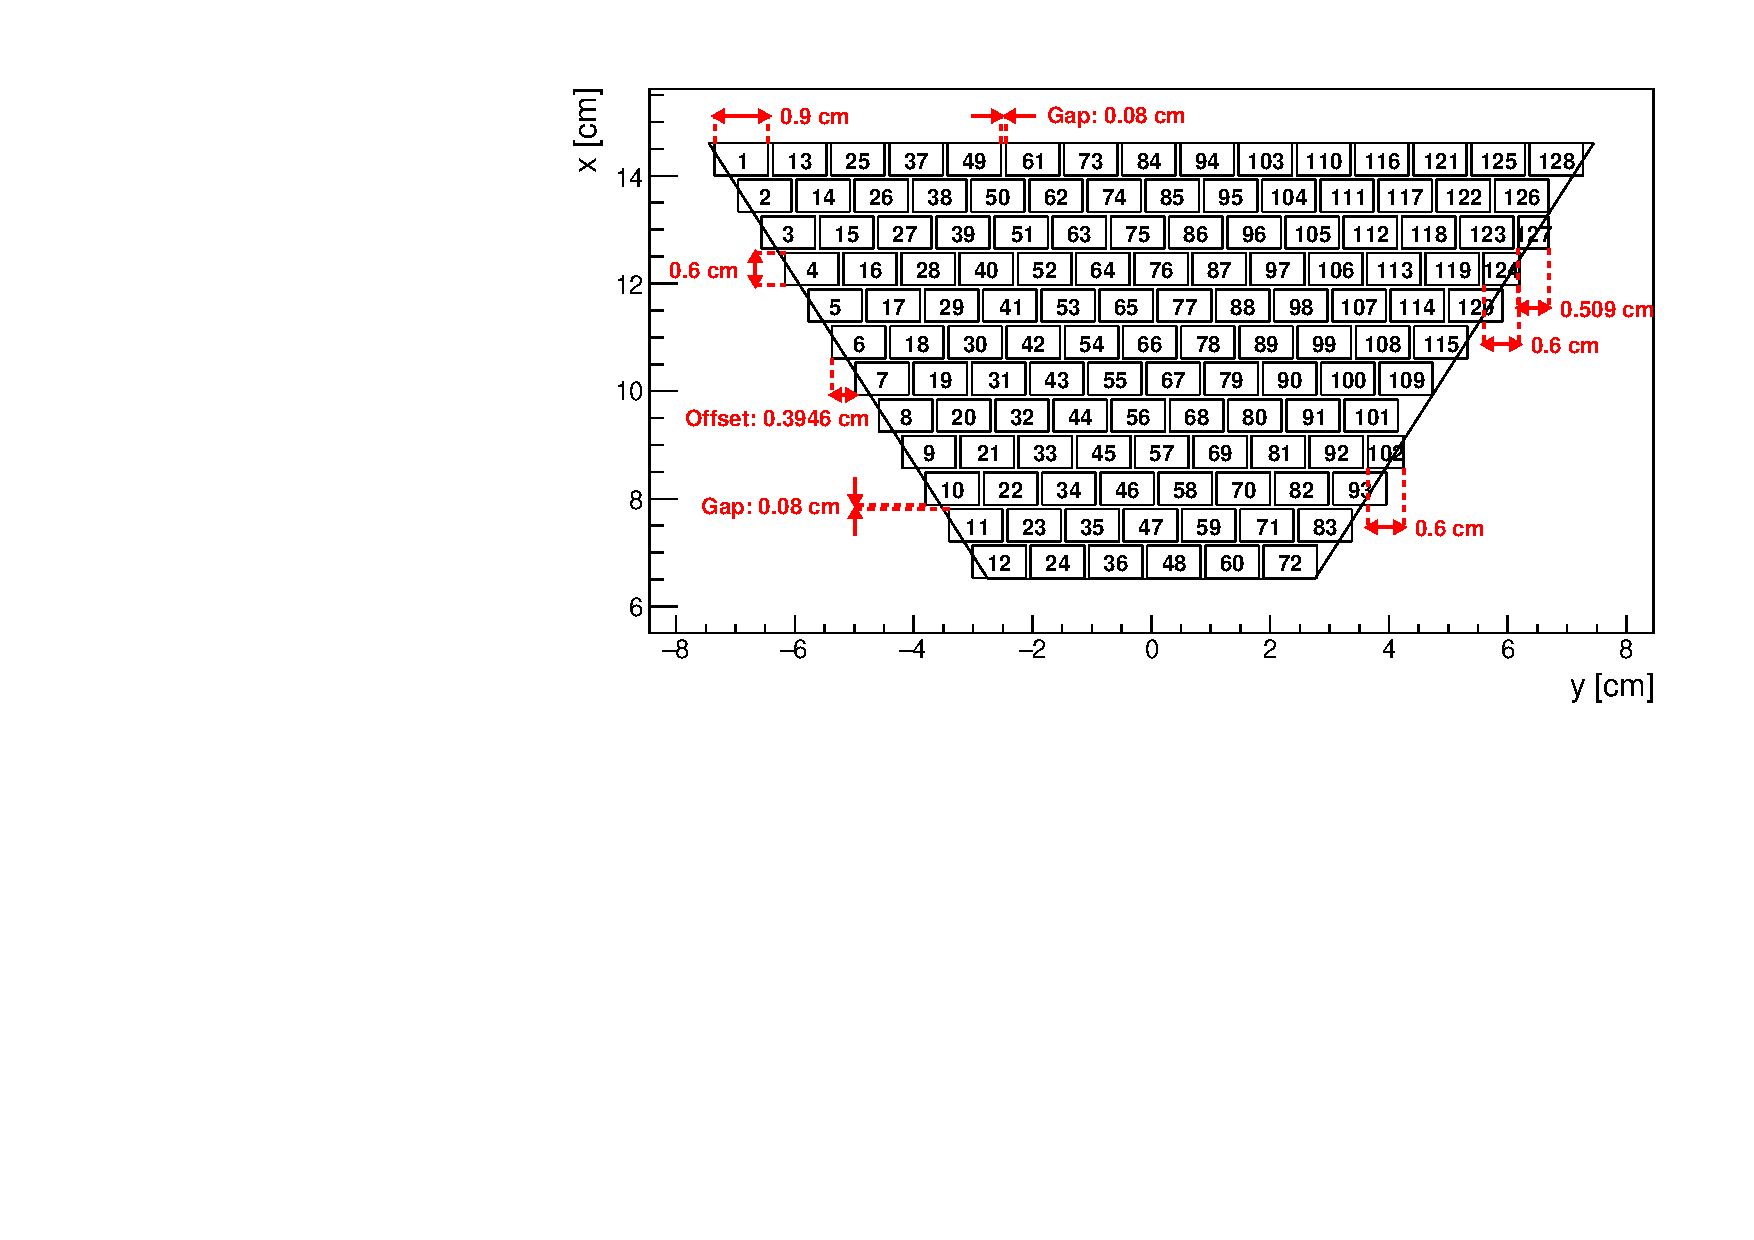
\includegraphics[width=\textwidth]{../../figures/pad_layout.pdf}
	\end{frame}
	}
	
	\begin{frame}
		\frametitle{OFTPC: Complications}
		Inhomogeneous magnetic field (simulated using Maxwell~\cite{ansys_maxwell})
		\begin{columns}
			\column{0.42\textwidth}
			\centering
			\begin{minipage}[t][4cm]{\textwidth}
				\centering
				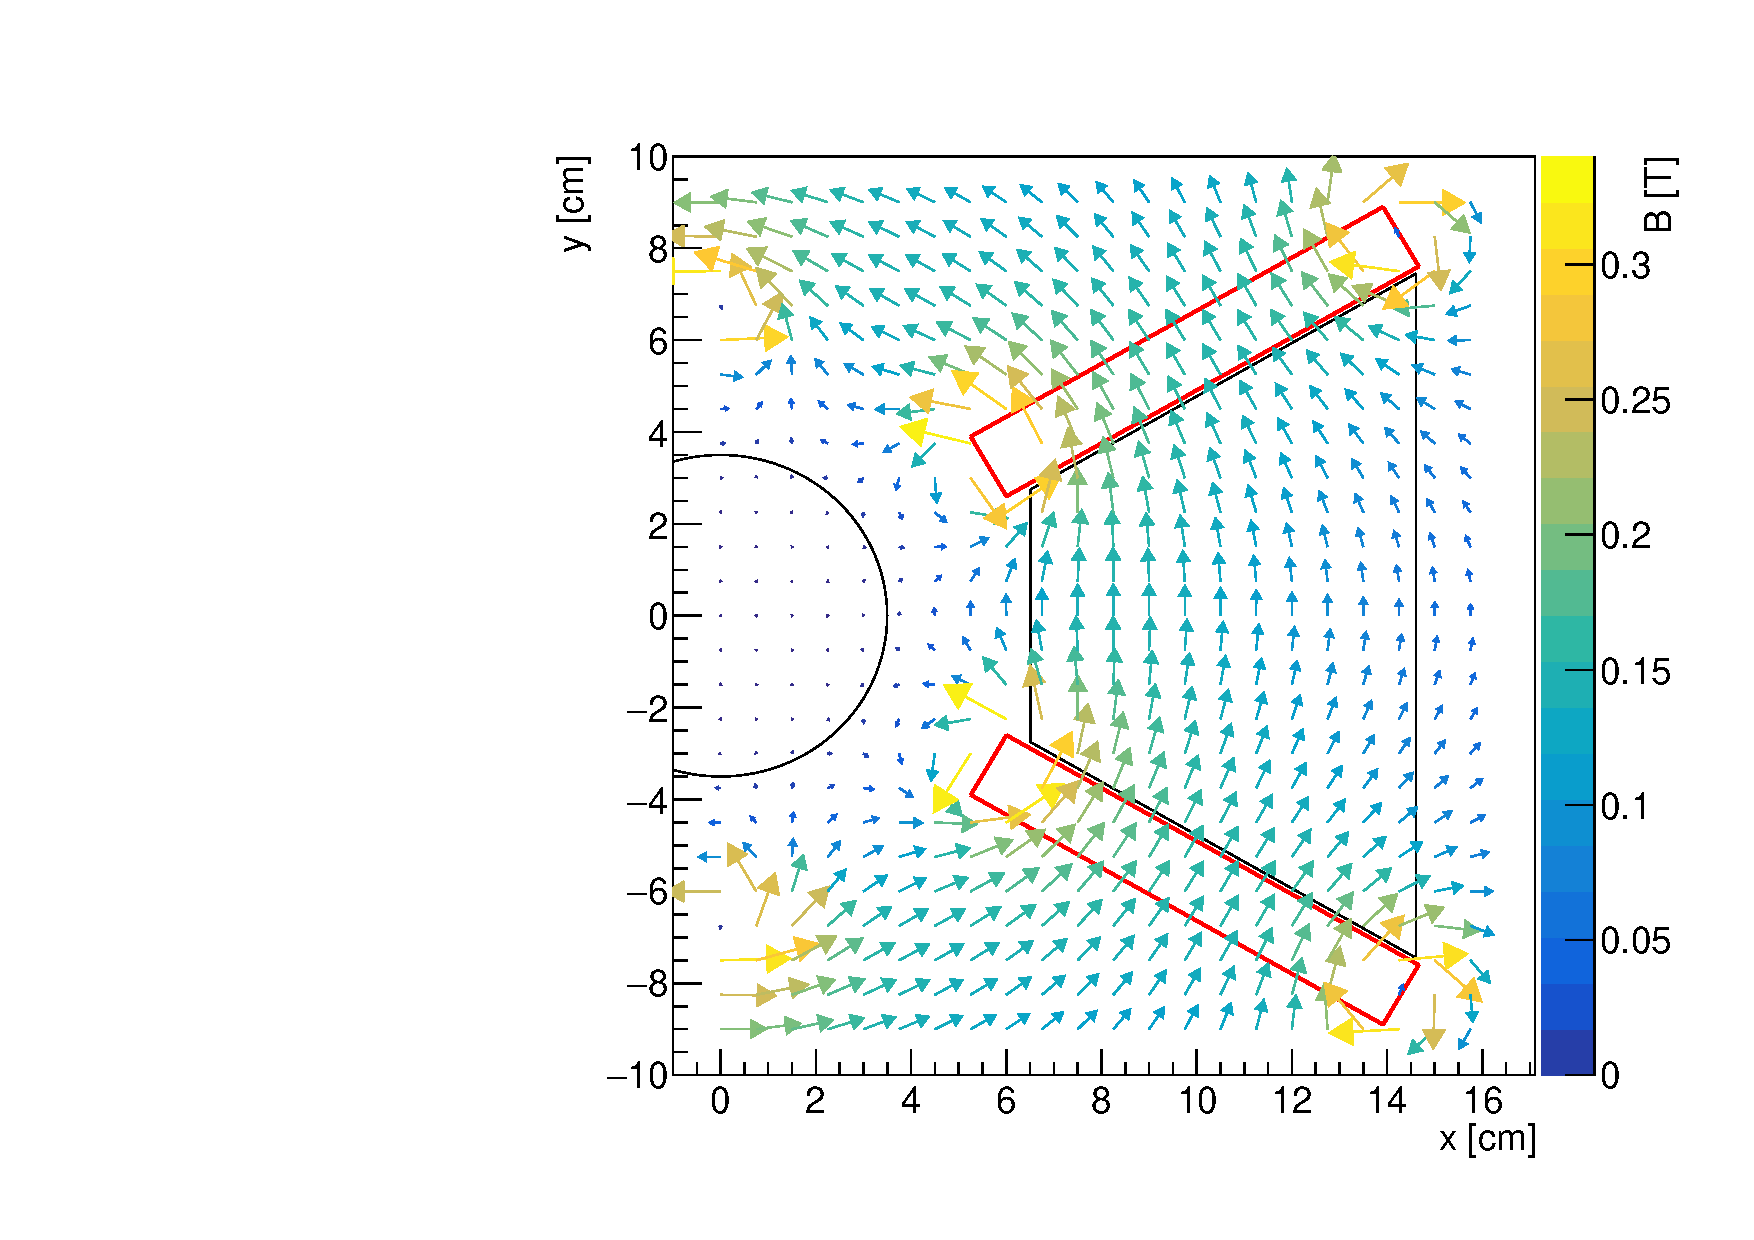
\includegraphics[width = \textwidth]{../../figures/tpc_mag_xy.pdf}
			\end{minipage}
			\column{0.58\textwidth}
			\centering
			\begin{minipage}[t][4cm]{\textwidth}
				\centering
				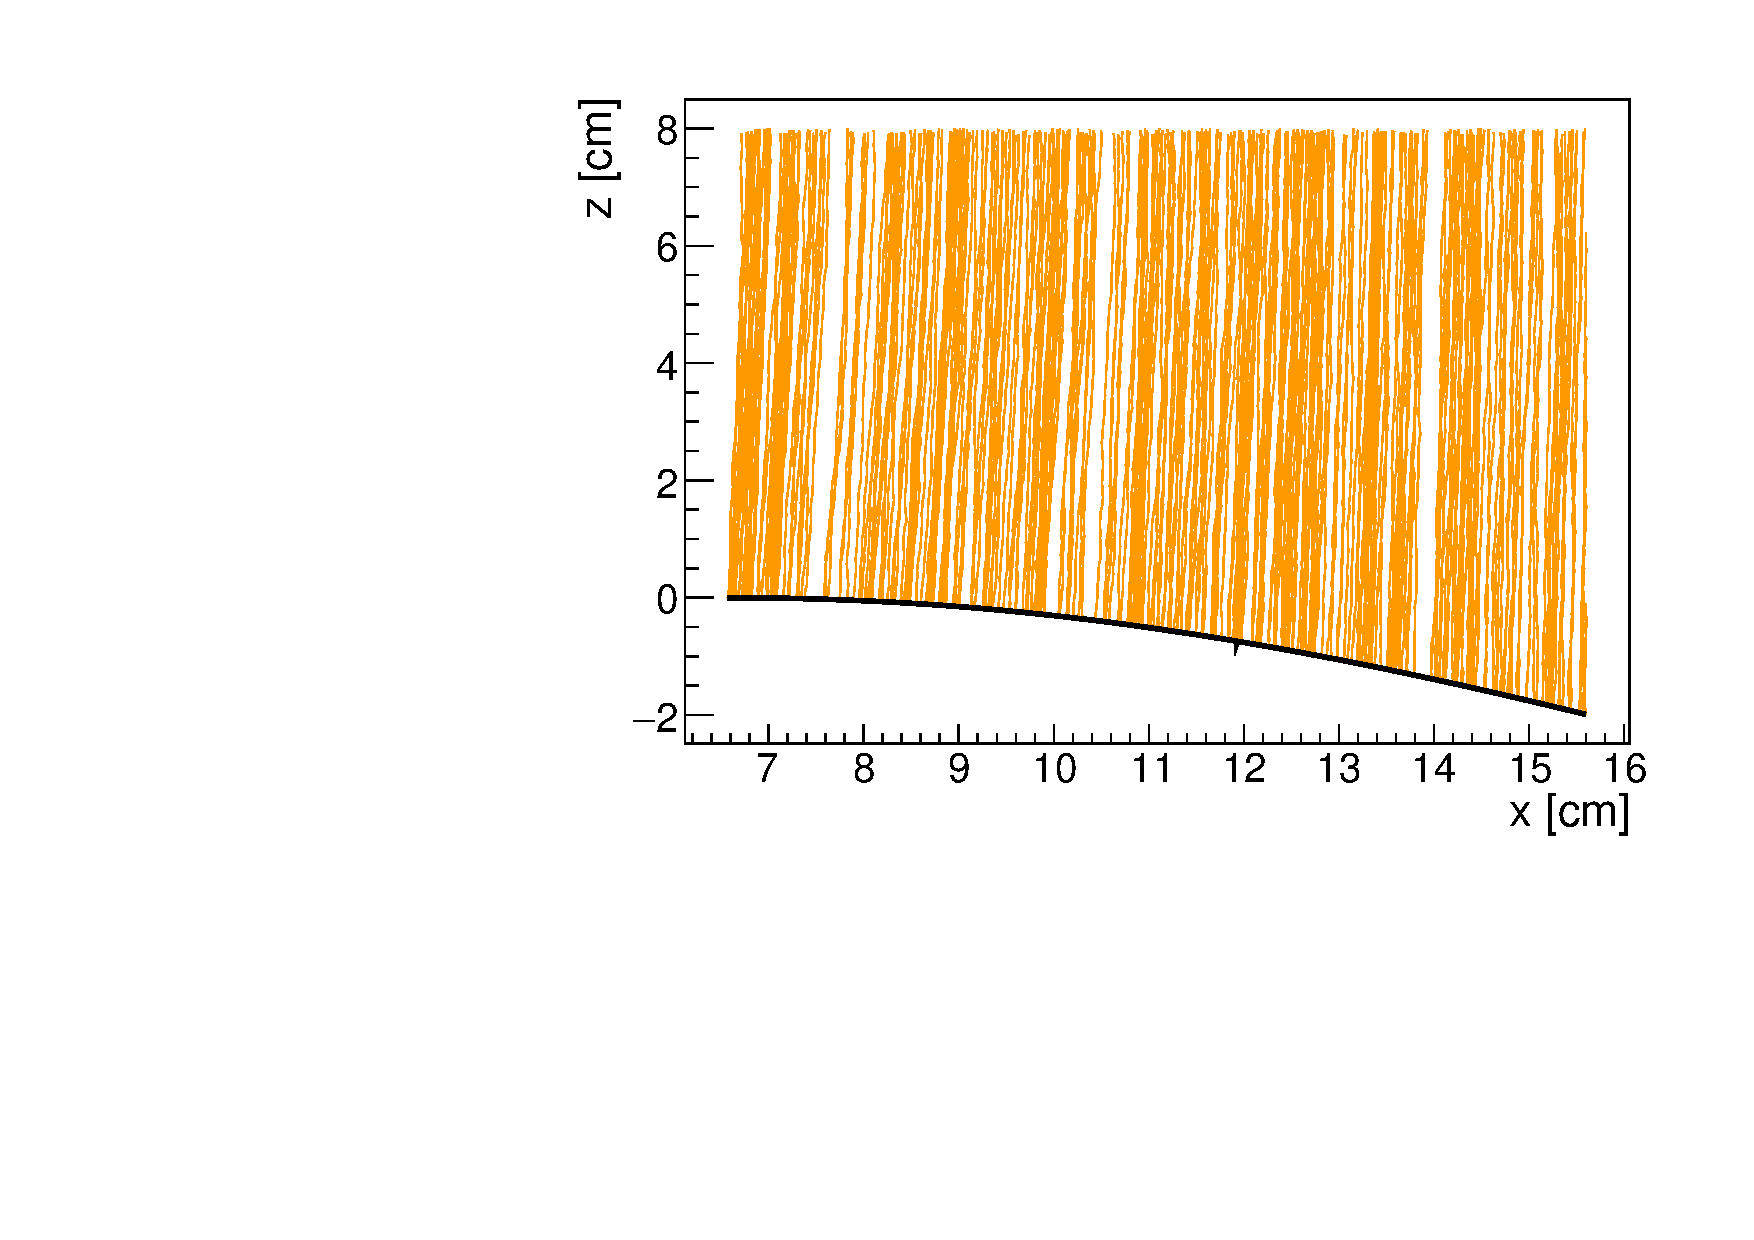
\includegraphics[width = 0.95 \textwidth]{../../figures/drift_7030_xz_small.pdf}
			\end{minipage}
		\end{columns}
		\begin{itemize}
			\item The field interferes with the direction of the drift of ionization electrons (position dependent Lorentz angle)
			\item Curvature of the track is not constant in this field\\ (deviation from a~circle)
		\end{itemize}
	\end{frame}
	
	\section{Track Simulation}
	{\nologo
	\begin{frame}
		\frametitle{Track Simulation: Initial Approach}
		\begin{itemize}
			\item At first simplified Garfield++ simulation (HEED, \texttt{AvalancheMicroscopic})
			\item Five batches of 9702 tracks with different initial parameters simulated on a grid (MetaCentrum~\cite{metacentrum})
			\begin{itemize}
				\item Electrons and positrons
				\item 11 different energies from 3~MeV to 13~MeV (covers range for $ {}^8\text{Be} $)
				\item 21 different angles~$\varphi$ and 21 different angles~$\theta$
			\end{itemize}
			\item Example $e^-$ track with kinetic energy 8~MeV, $\theta = 0^\circ$ and $\varphi = 0^\circ$
			\item Diffusion less than 1.5~mm in both directions
		\end{itemize}
		\begin{columns}
			\column{0.33\textwidth}
			\centering
			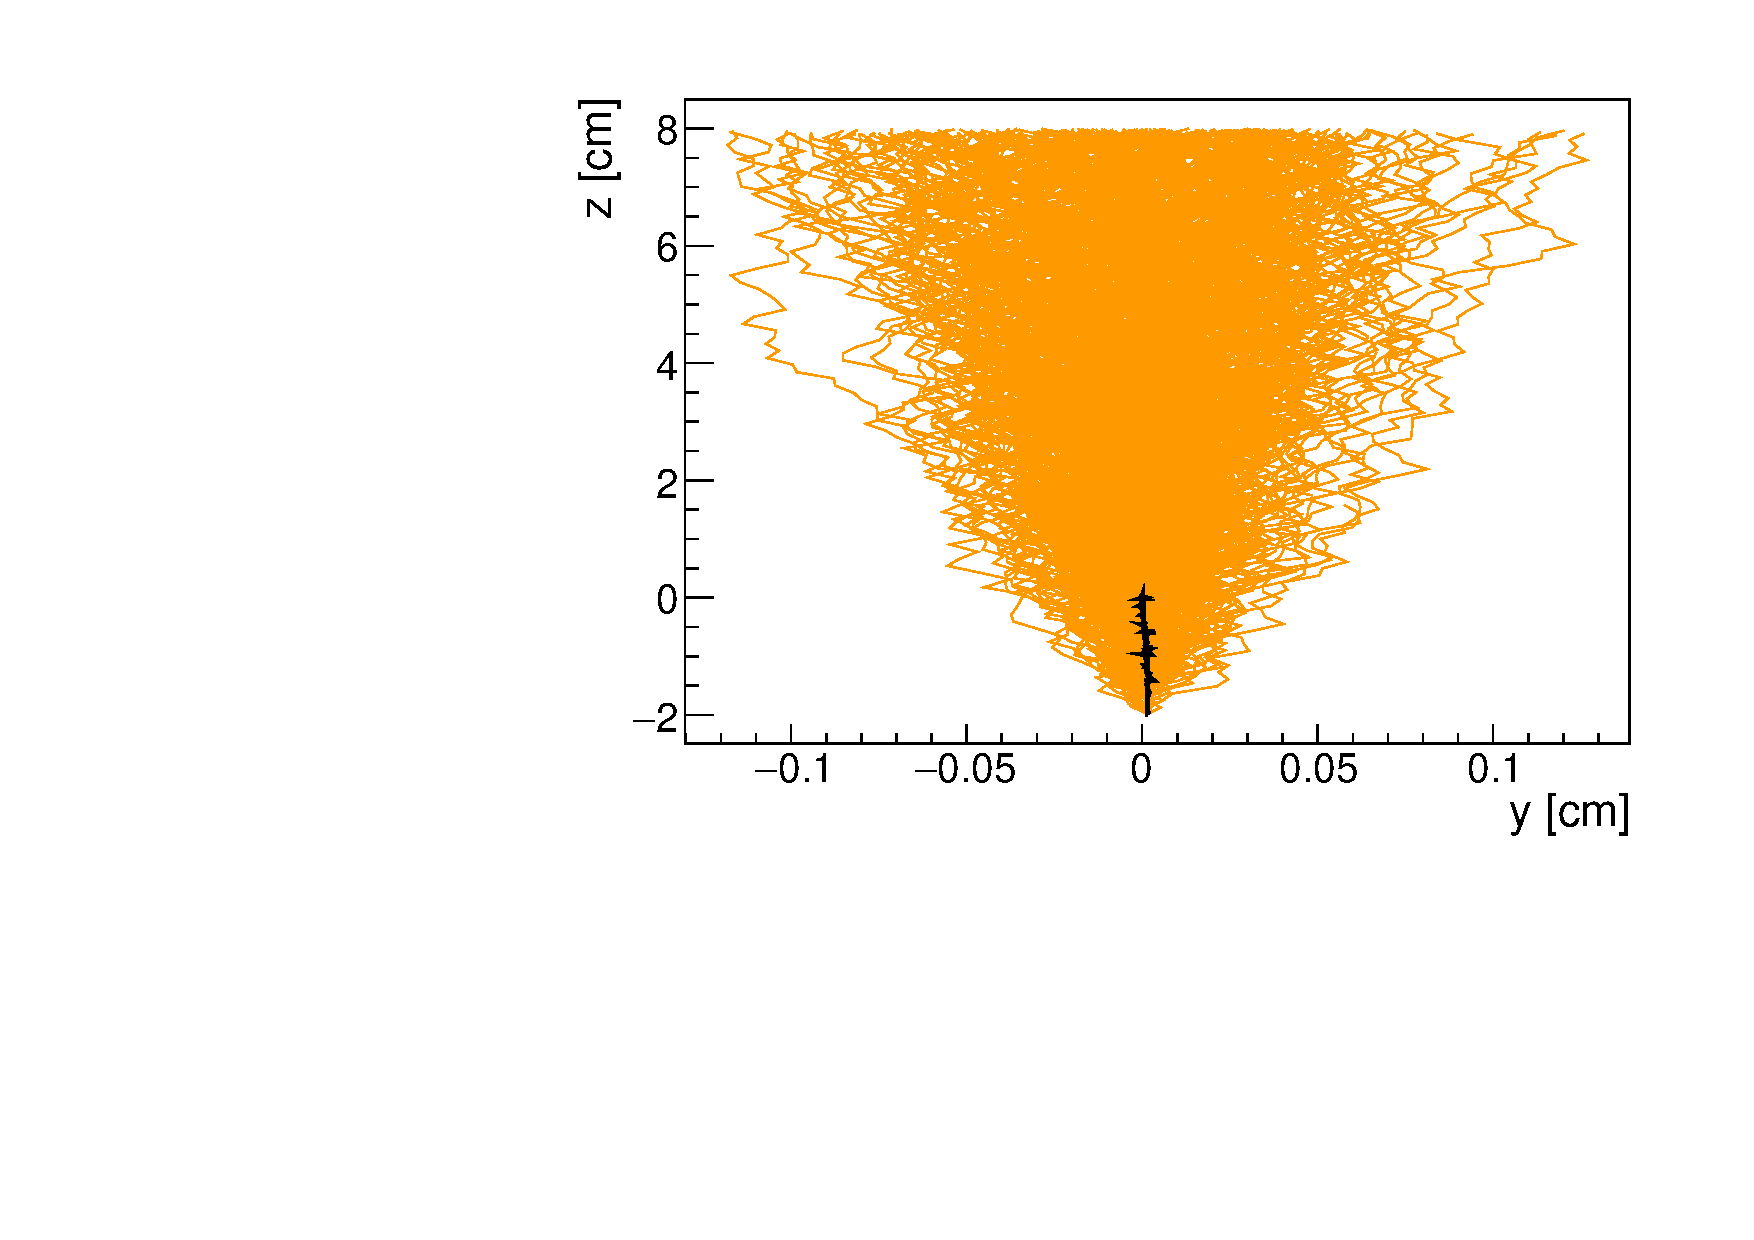
\includegraphics[width = 0.97 \linewidth]{../../figures/drift_7030_yz_small.pdf}
			Diffusion front view
			\column{0.33\textwidth}
			\centering
			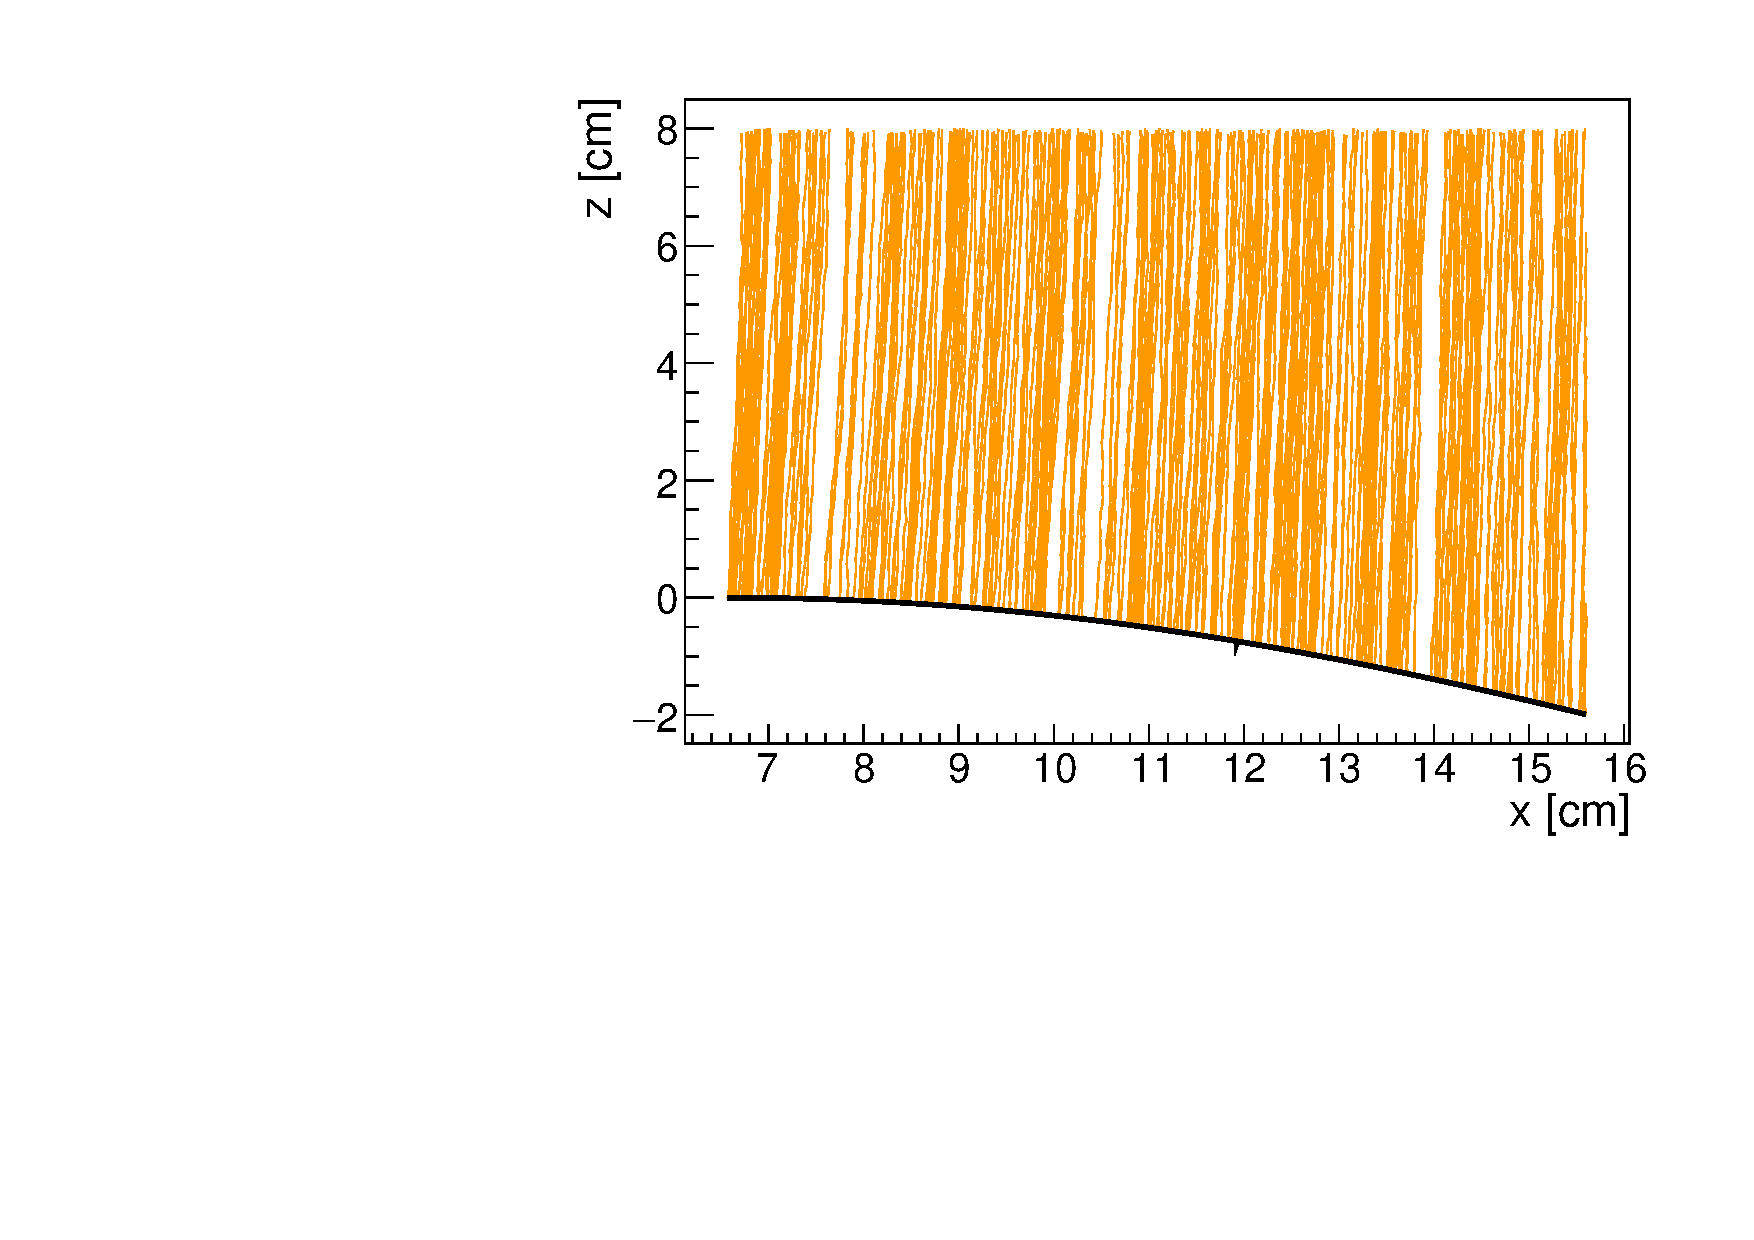
\includegraphics[width = 0.97 \linewidth]{../../figures/drift_7030_xz_small.pdf}
			Electron drift
			\column{0.33\textwidth}
			\centering
			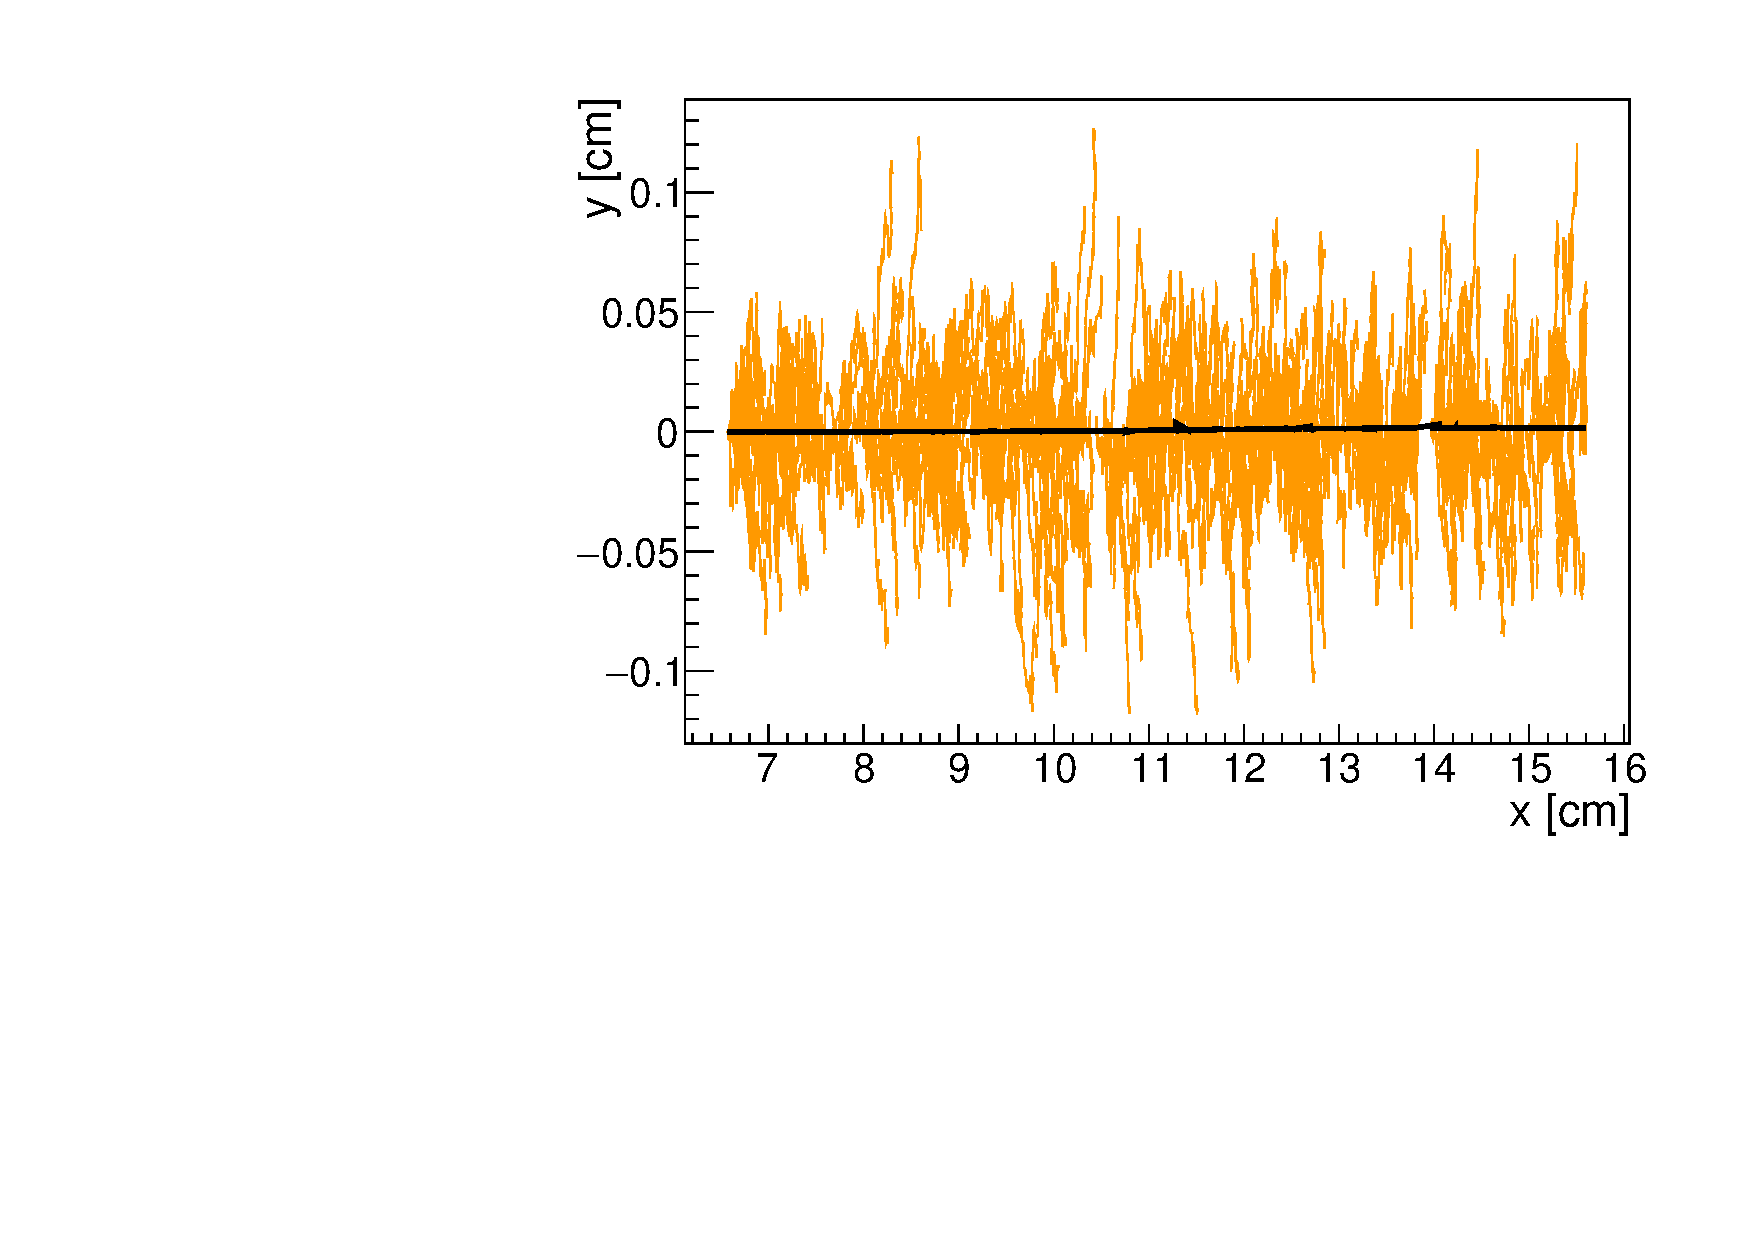
\includegraphics[width = 0.97 \linewidth]{../../figures/drift_7030_xy_small.pdf}
			Diffusion top view
		\end{columns}
	\end{frame}
	}
	
	{\nonav
	\begin{frame}
		\frametitle{Ionization Electron Map Simulation}
		\begin{itemize}
			\item We want an~unambiguous map of the drift of ion. $e^-$ for the reconstr.
			\item We can use a~simulation of evenly spaced electrons
			\begin{itemize}
				\item Current spacing 5~mm, 100 electrons simulated in each location with 0.1~eV energy in a~random direction
			\end{itemize}
			\item Result = mapping from initial coor. $(x,y,z)$ to readout $(x',y',t)$
			\item Inverse map used for reconstruction of track voxels
		\end{itemize}
		\begin{columns}
			\column{0.06\textwidth}
			\column{0.44\textwidth}
			\centering
			\begin{minipage}[t][4.2cm]{\textwidth}
				\centering
				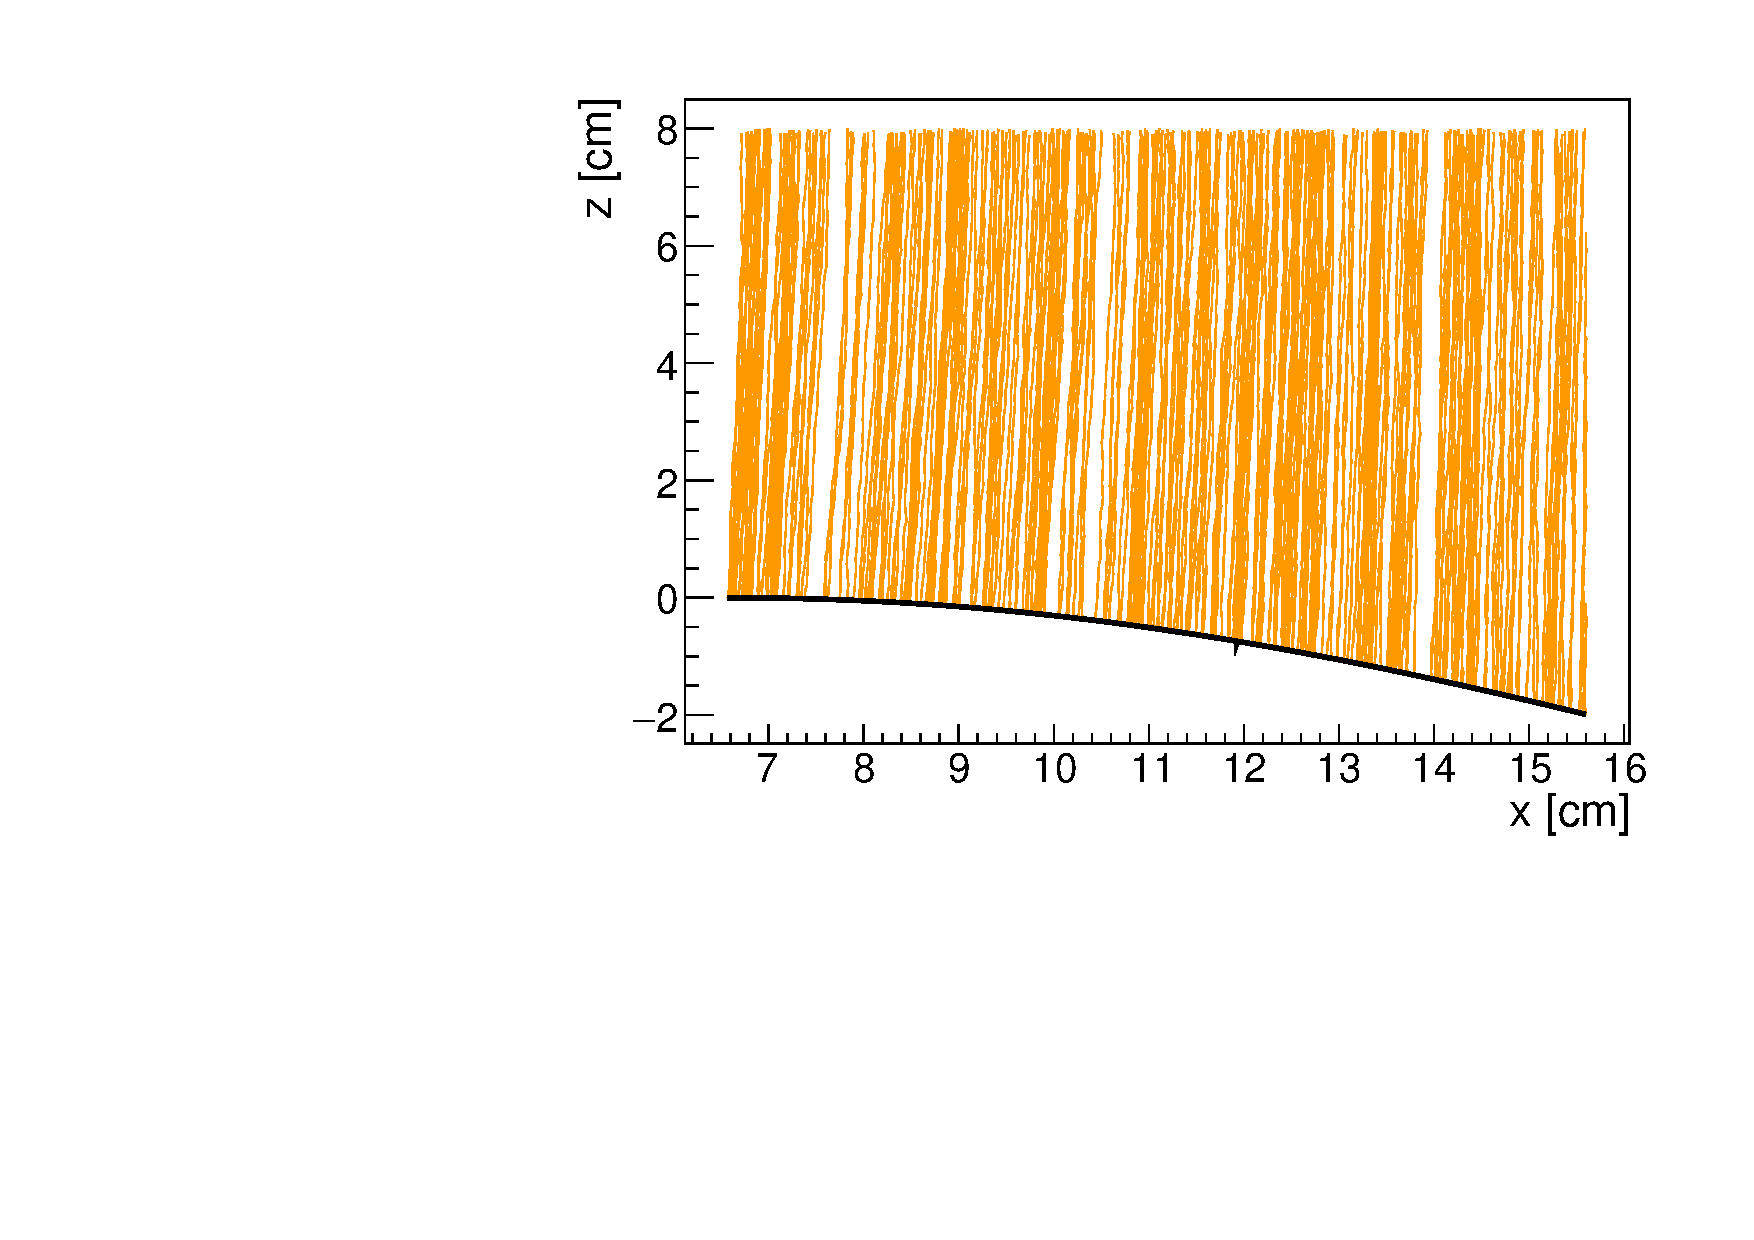
\includegraphics[width = \textwidth]{../../figures/drift_7030_xz_small.pdf}\\
			\end{minipage}
			\small{Electron drift}
			\column{0.44\textwidth}
			\centering
			\begin{minipage}[t][4.2cm]{\textwidth}
				\centering
				\includegraphics[width=0.7\textwidth]{figures/map_lines.png}\\
			\end{minipage}
			\small{Partial simulation of the map}
			\column{0.06\textwidth}
		\end{columns}
	\end{frame}
	}
	\begin{frame}
		\frametitle{Ionization Electron Map Simulation: Visualization}
		\begin{figure}
			\centering
			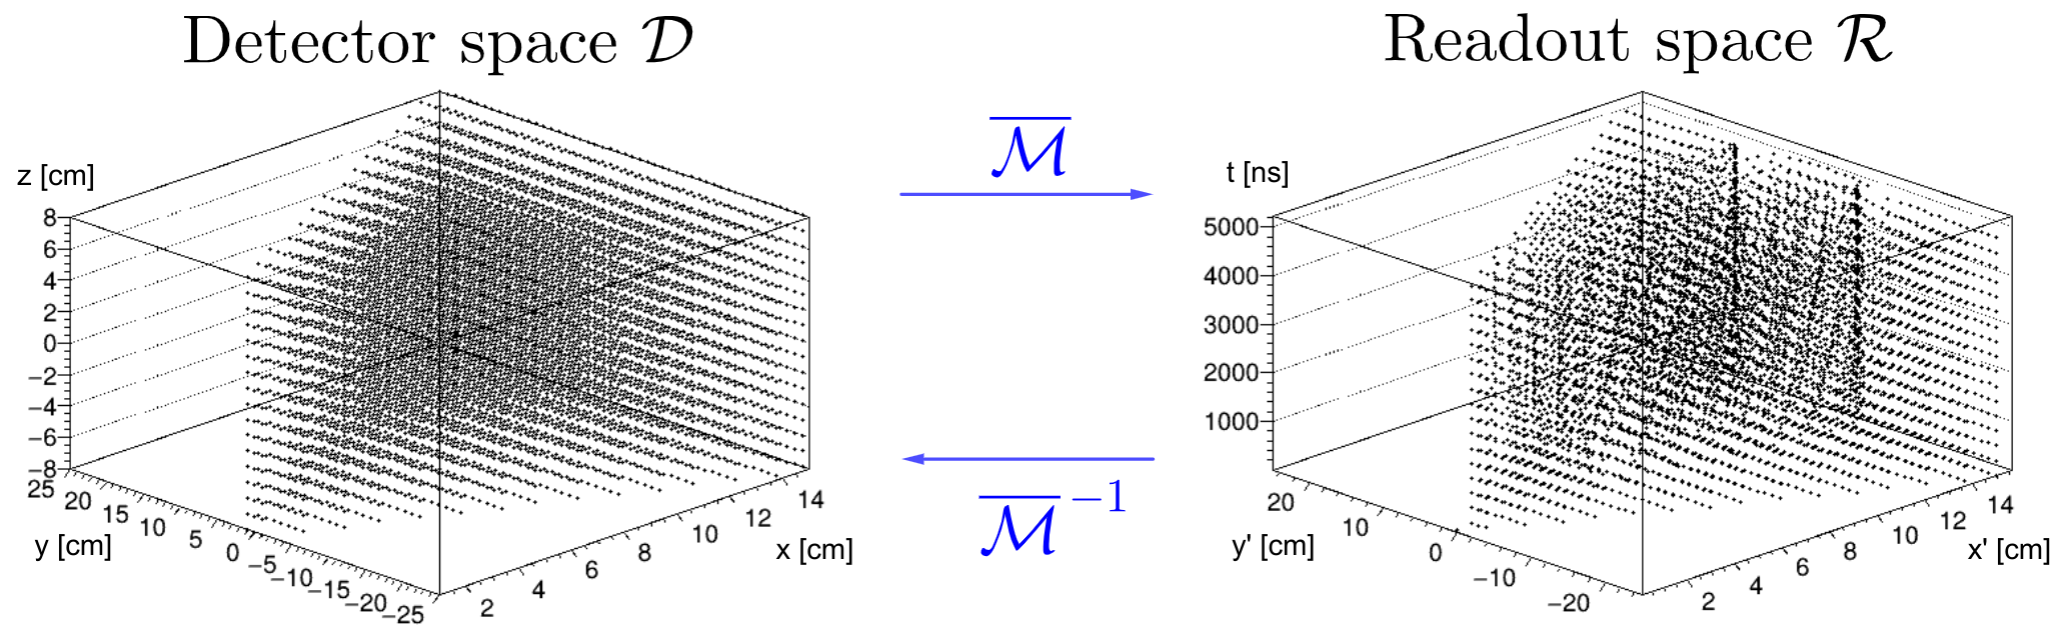
\includegraphics[width=\textwidth]{figures/map_3dvis.png}
			\small{3D visualization of the simulated mapping $\overline{\mathcal{M}}$ and the inverse mapping $\overline{\mathcal{M}}^{-1}$.}
		\end{figure}
	\end{frame}

	\begin{frame}
		\frametitle{Ionization Electron Map Simulation: Diffusion}
		\centering
		\begin{minipage}[c]{0.9\textwidth}
			\begin{figure}
				\centering
				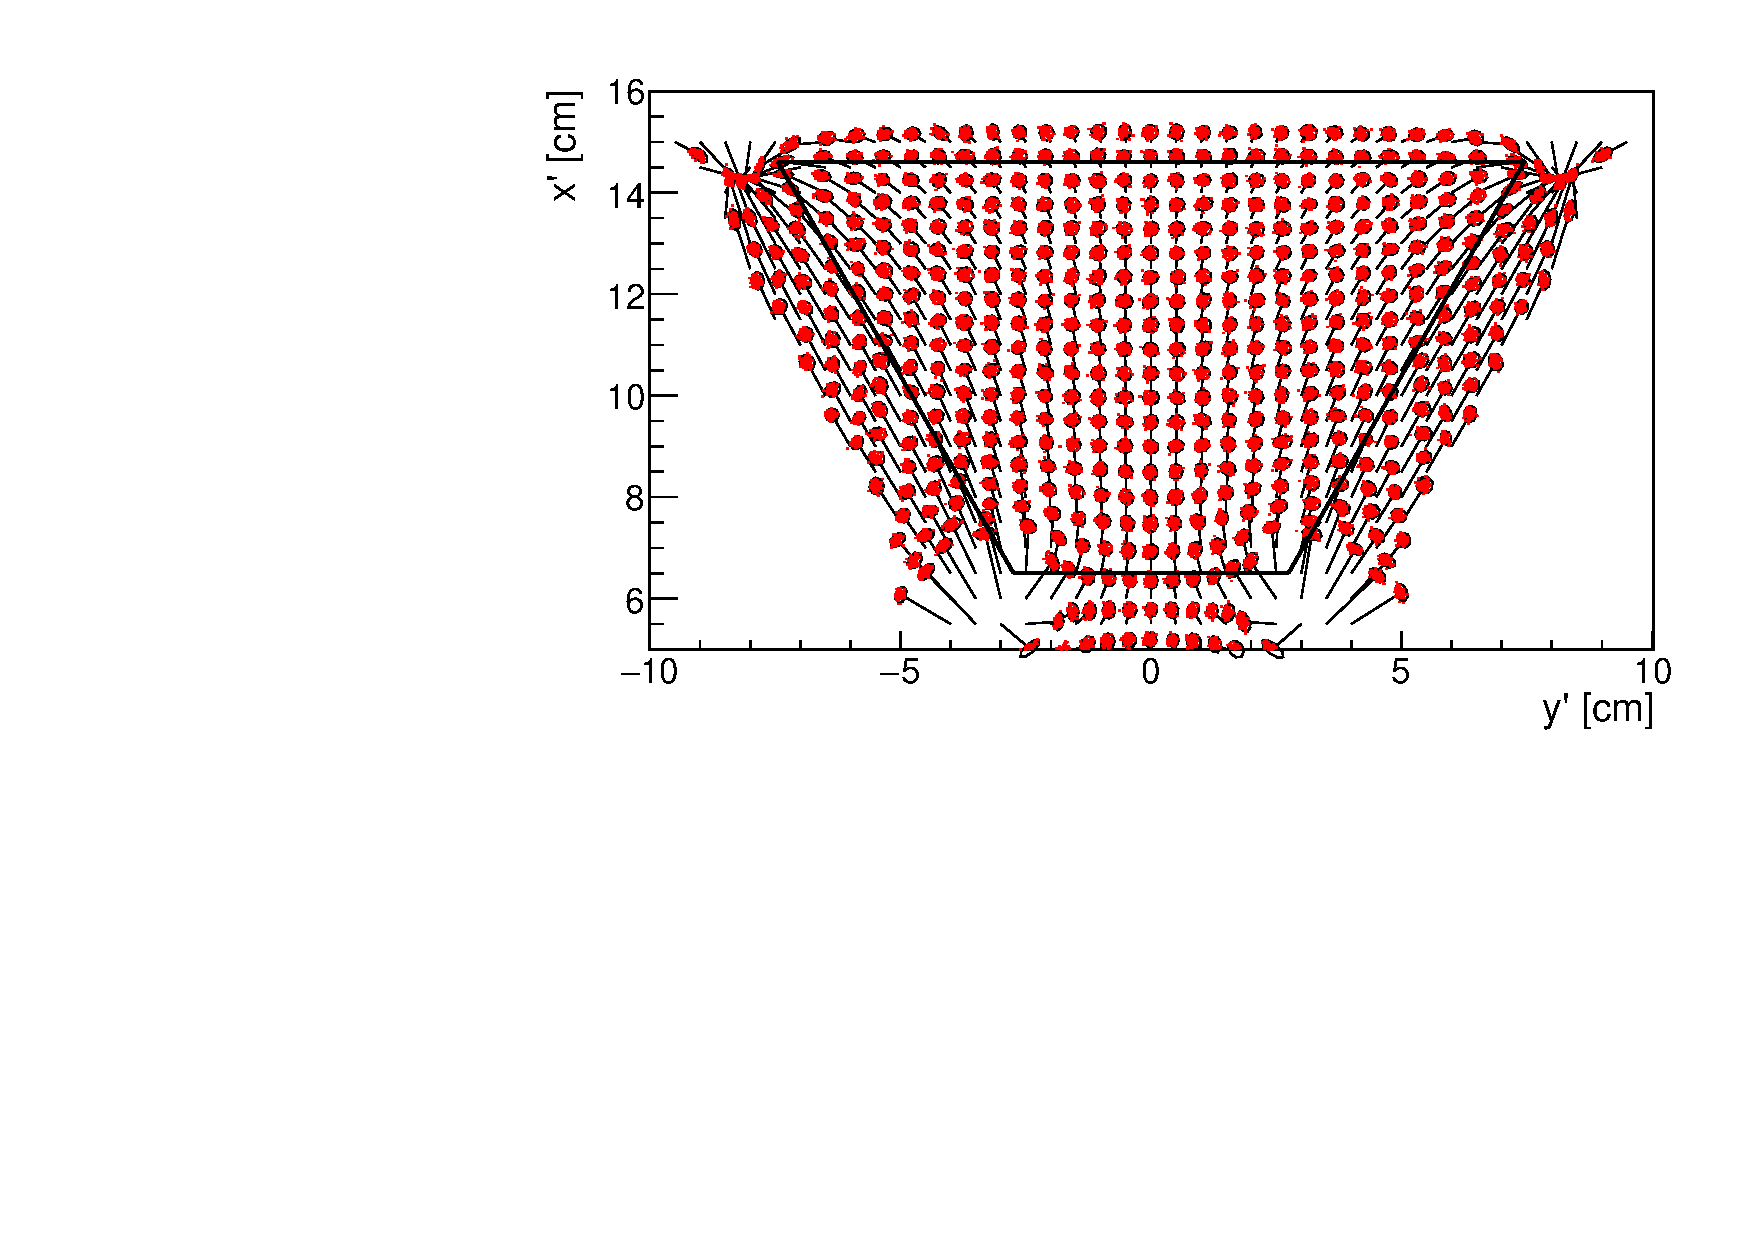
\includegraphics[height=0.7\textheight]{../../figures/map_yx_bottom.pdf}\\
				\small{Worst case $x$ and $y$ coordinate distortion for maximal initial distance from readout. Ellipses  with 95~\% confidence are shown for each starting position.}
			\end{figure}
		\end{minipage}
	\end{frame}
	
	{\nonav
	\begin{frame}
		\frametitle{Track Simulation: Multiple Scattering}
		\begin{itemize}
			\item HEED does not account for multiple scattering of relativistic primaries in the gas mixture.
			\item At relatively low $e^+$/$e^-$ energies of 3--13~MeV, it can significantly distort the trajectory.
			\item Therefore, we are implementing a Geant4-\garfieldpp\ interface (inspired by Pfeiffer et al.~\cite{interface}). Preliminary tests were done.
		\end{itemize}
		\centering
		\begin{minipage}[c]{0.8\textwidth}
			\begin{figure}
				\centering
				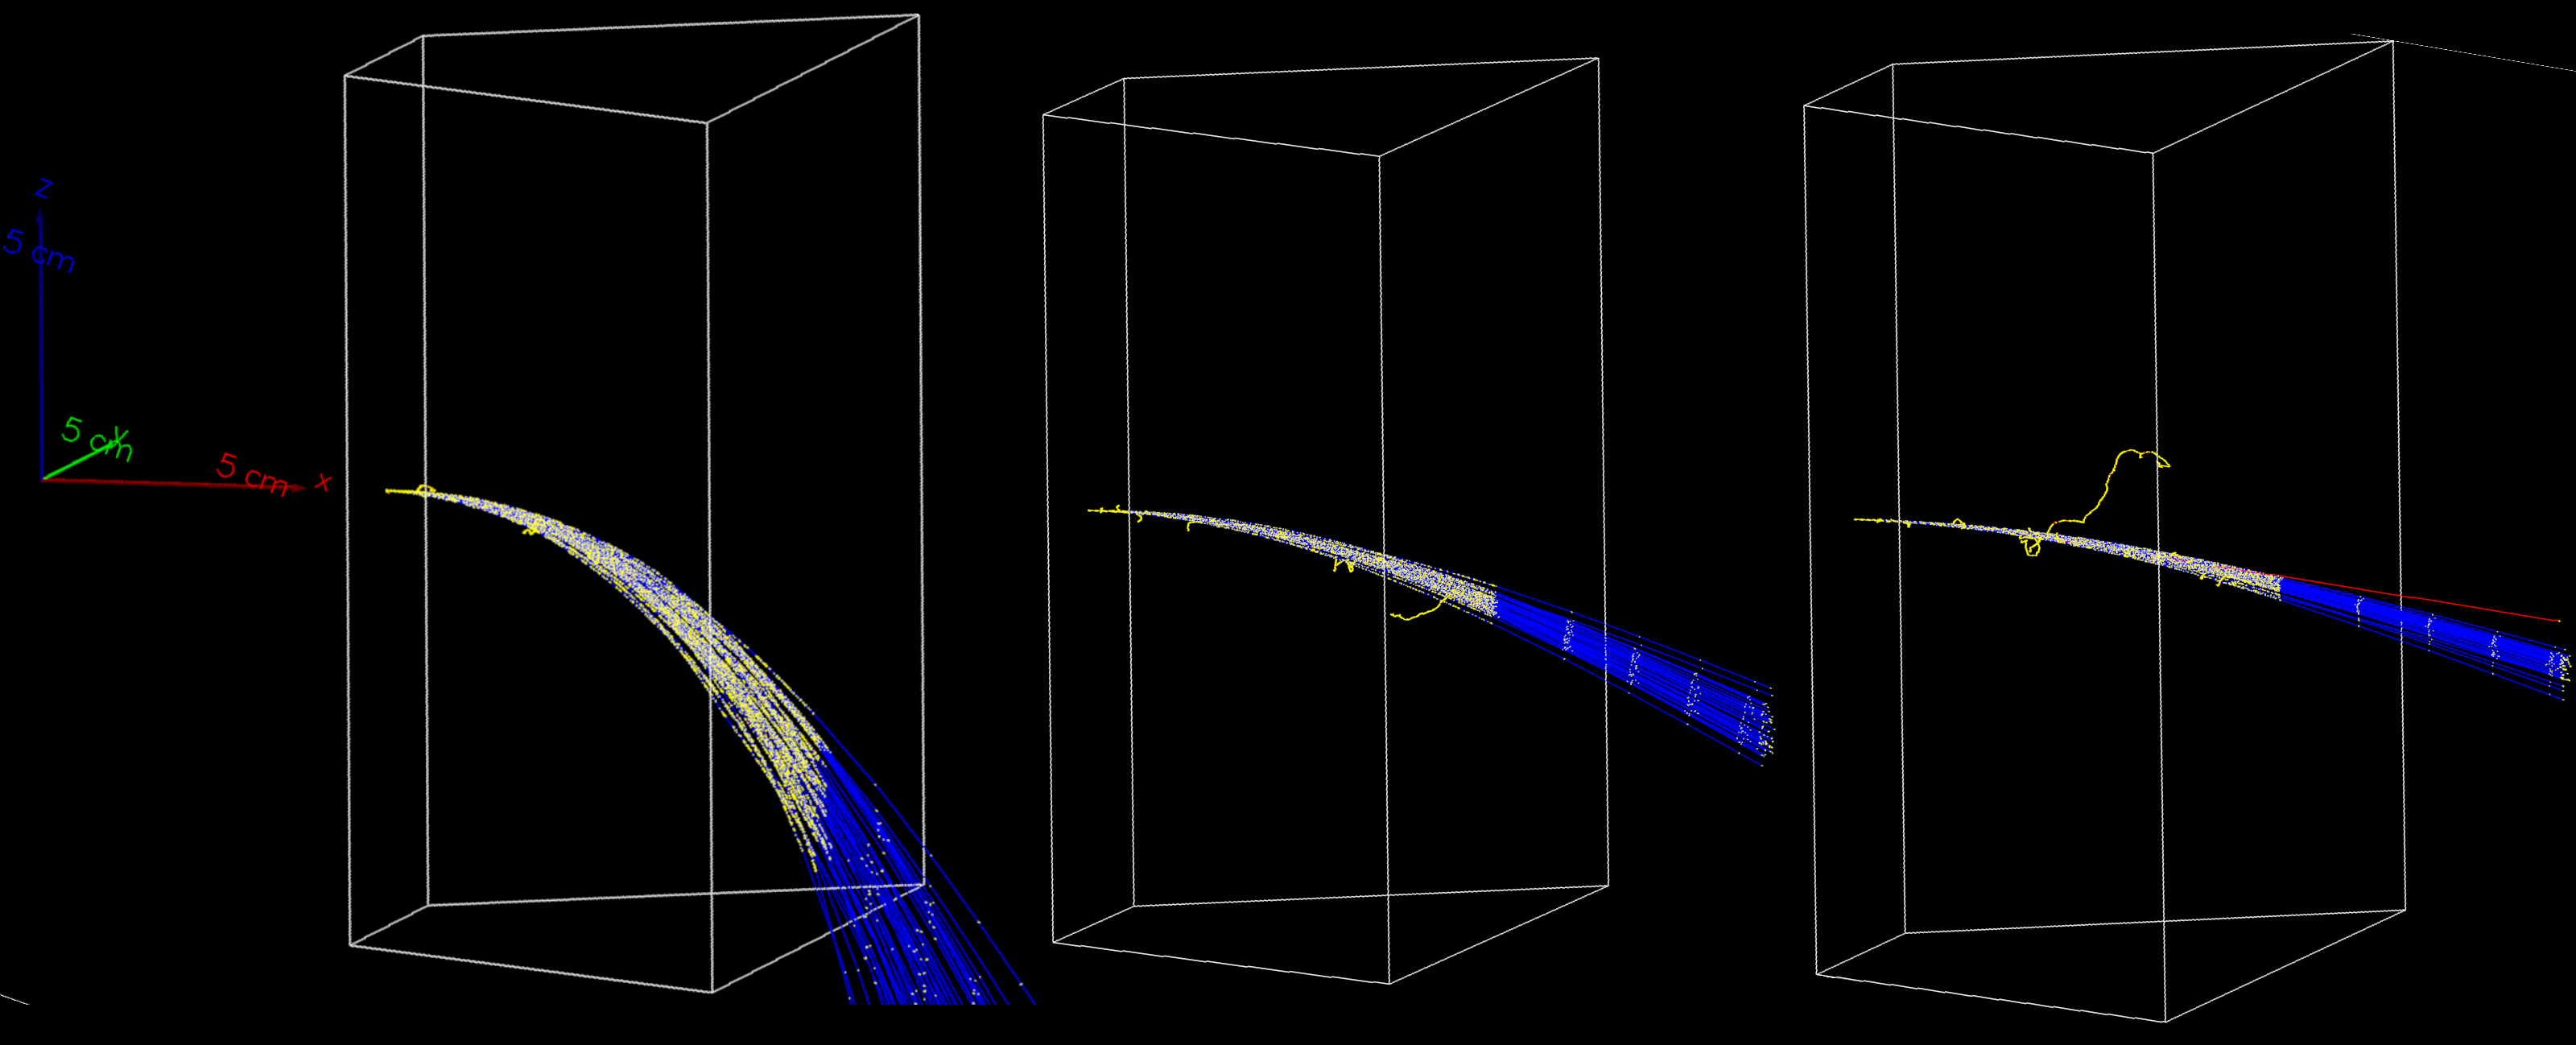
\includegraphics[width=\textwidth]{../../figures/mcs_triple.png}\\
				\small{Visualization three sets of 50 electron tracks with zero initial angles $\theta,\varphi$ and energies 3, 8, and 13~MeV.}
			\end{figure}
		\end{minipage}
	\end{frame}
 	}
	
	\section{Track Reconstruction}
	\begin{frame}
		\frametitle{Track Reconstruction}
		\begin{itemize}
			\item At first using only the inverse map (not accounting for readout pads)
			\item Later simple reconstruction with pads and time bins, counting the number of electrons in each bin
		\end{itemize}
		\begin{columns}
			\column{0.42\textwidth}
			\centering
			\begin{minipage}[t][4.5cm]{\textwidth}
				\centering
				\vspace{0.5cm}
				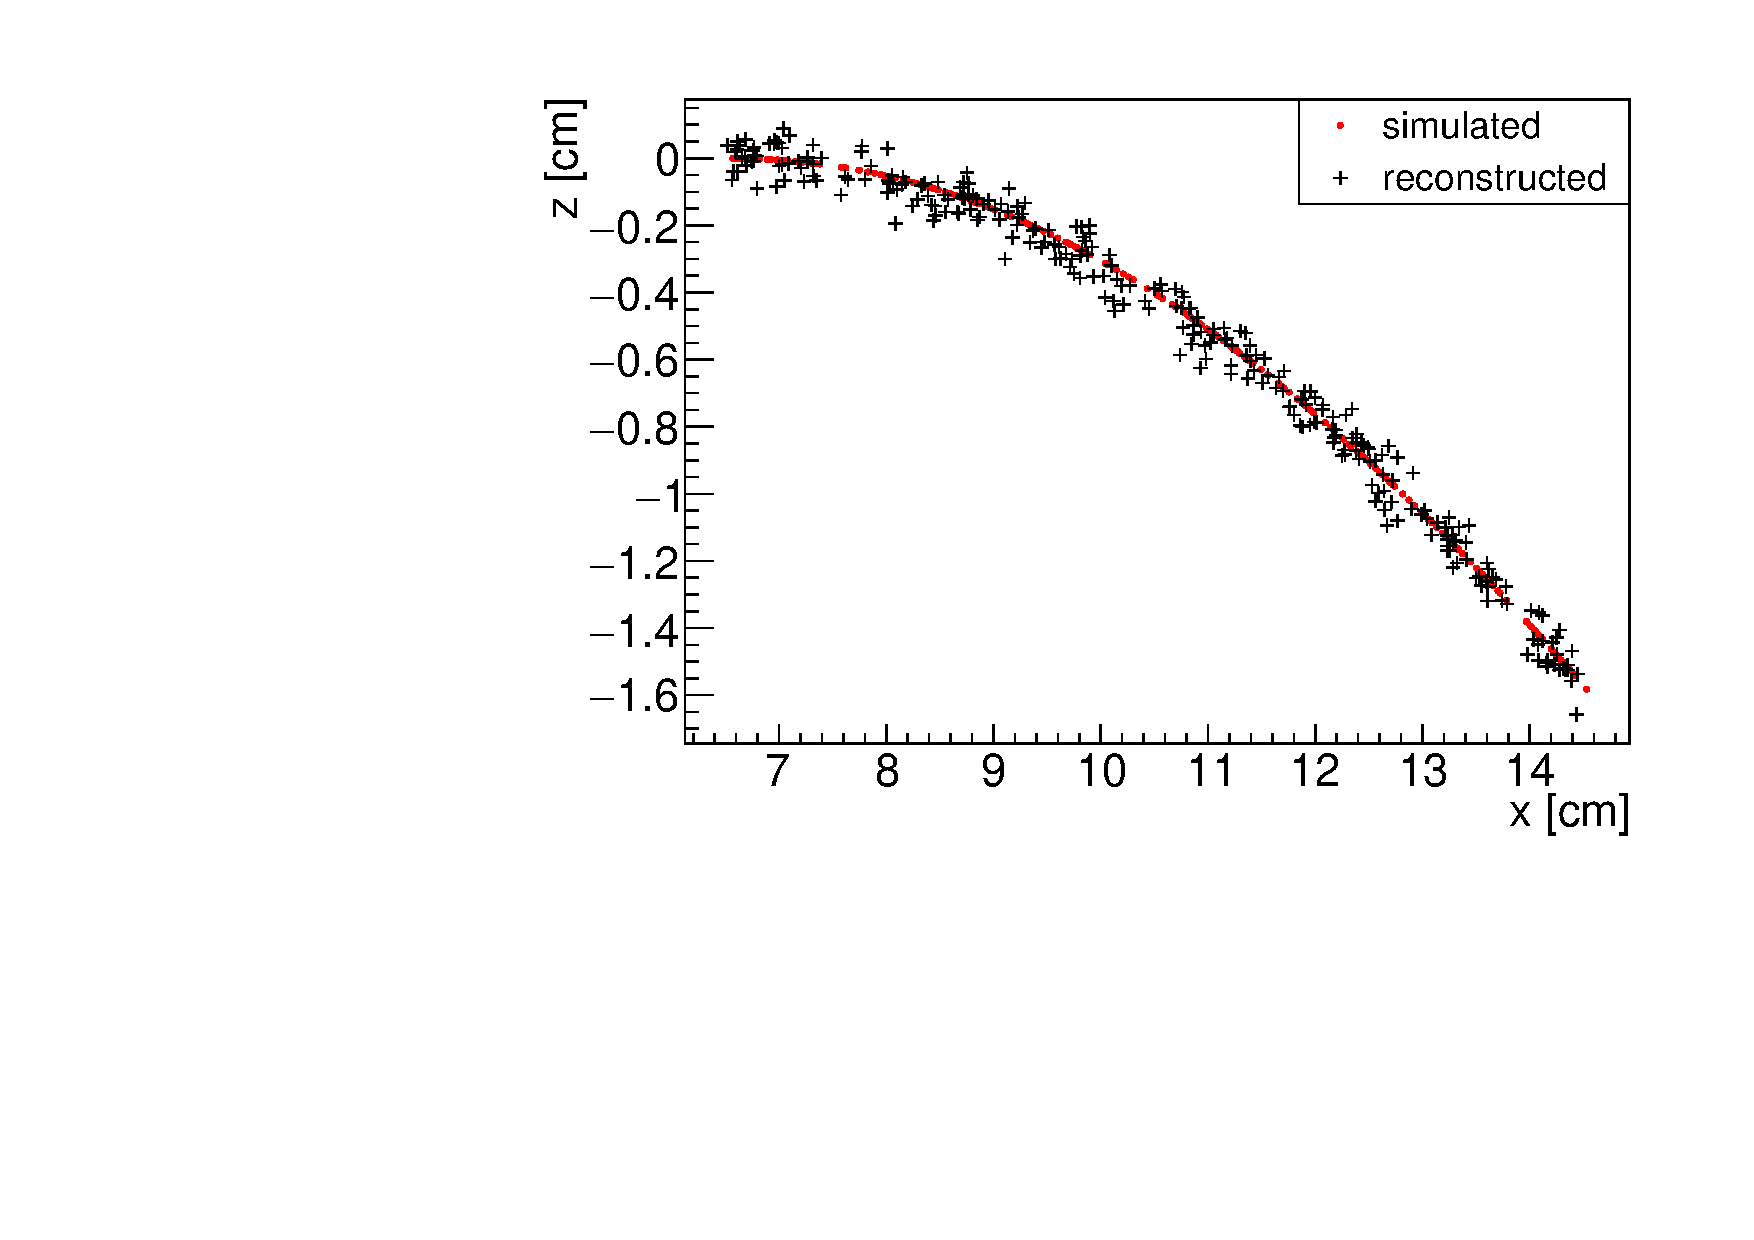
\includegraphics[width=\textwidth]{../../figures/7030_reco_map_xz.pdf}\\
			\end{minipage}
			\small{Original and reconstructed interaction points on the simulated track}
			\column{0.58\textwidth}
			\centering
			\begin{minipage}[t][4.5cm]{\textwidth}
				\centering
				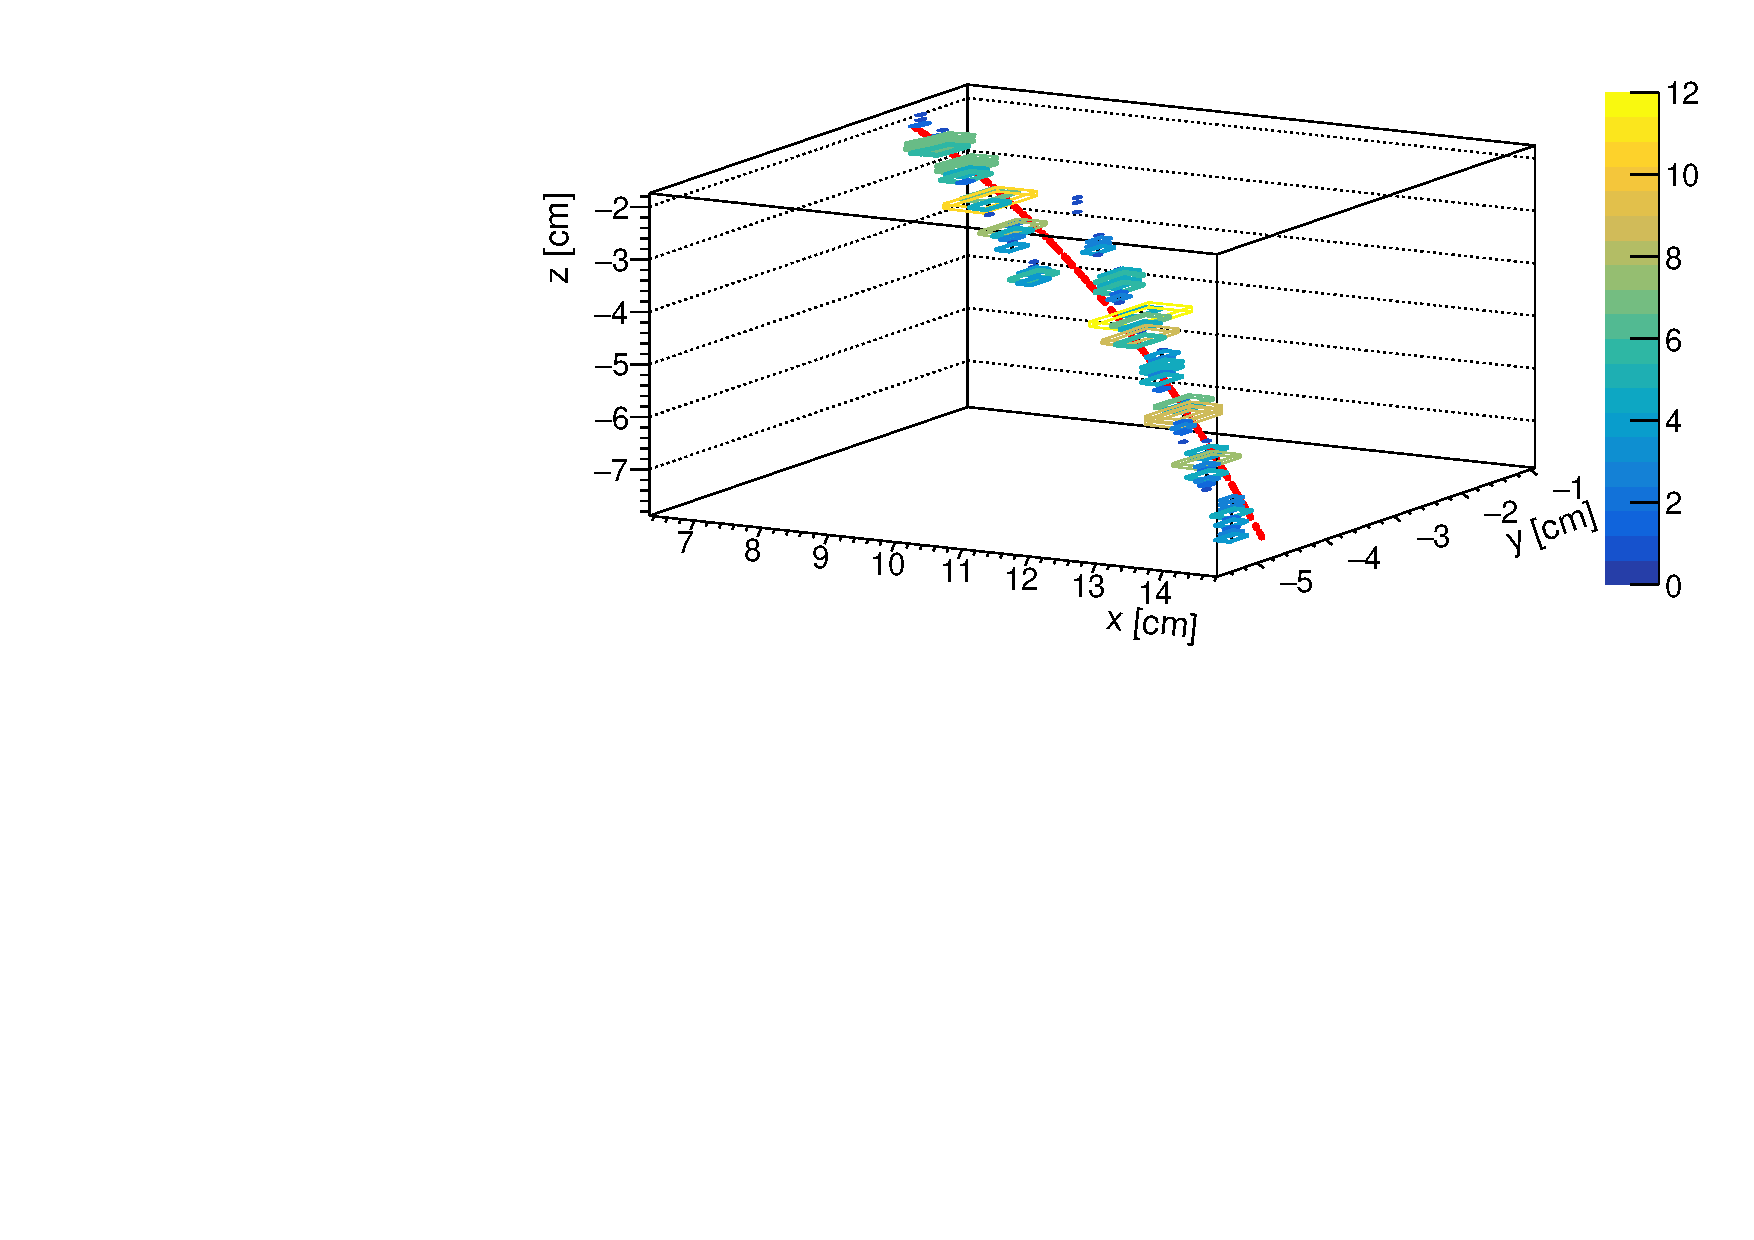
\includegraphics[width=\textwidth]{../../figures/track_padreco.pdf}\\
			\end{minipage}
			\small{Reconstruction with pads}
		\end{columns}
	\end{frame}
	
	\section{Energy Reconstruction}
	{\nonav
	\begin{frame}
		\frametitle{Energy Reconstruction}
		\begin{itemize}
			\item Prefit with circle with smoothly attached lines (blue)
			\item Kinetic energy fit using 4\textsuperscript{th} order Runge-Kutta (magenta)
			\item Known initial position and direction of the particle assumed
			\item Apply systematic error correction (\tiny{obtained from simulation using a 3D linear fit}\normalsize)
			\item Currently around 0.3~CPU seconds per track
		\end{itemize}
		
		\centering
		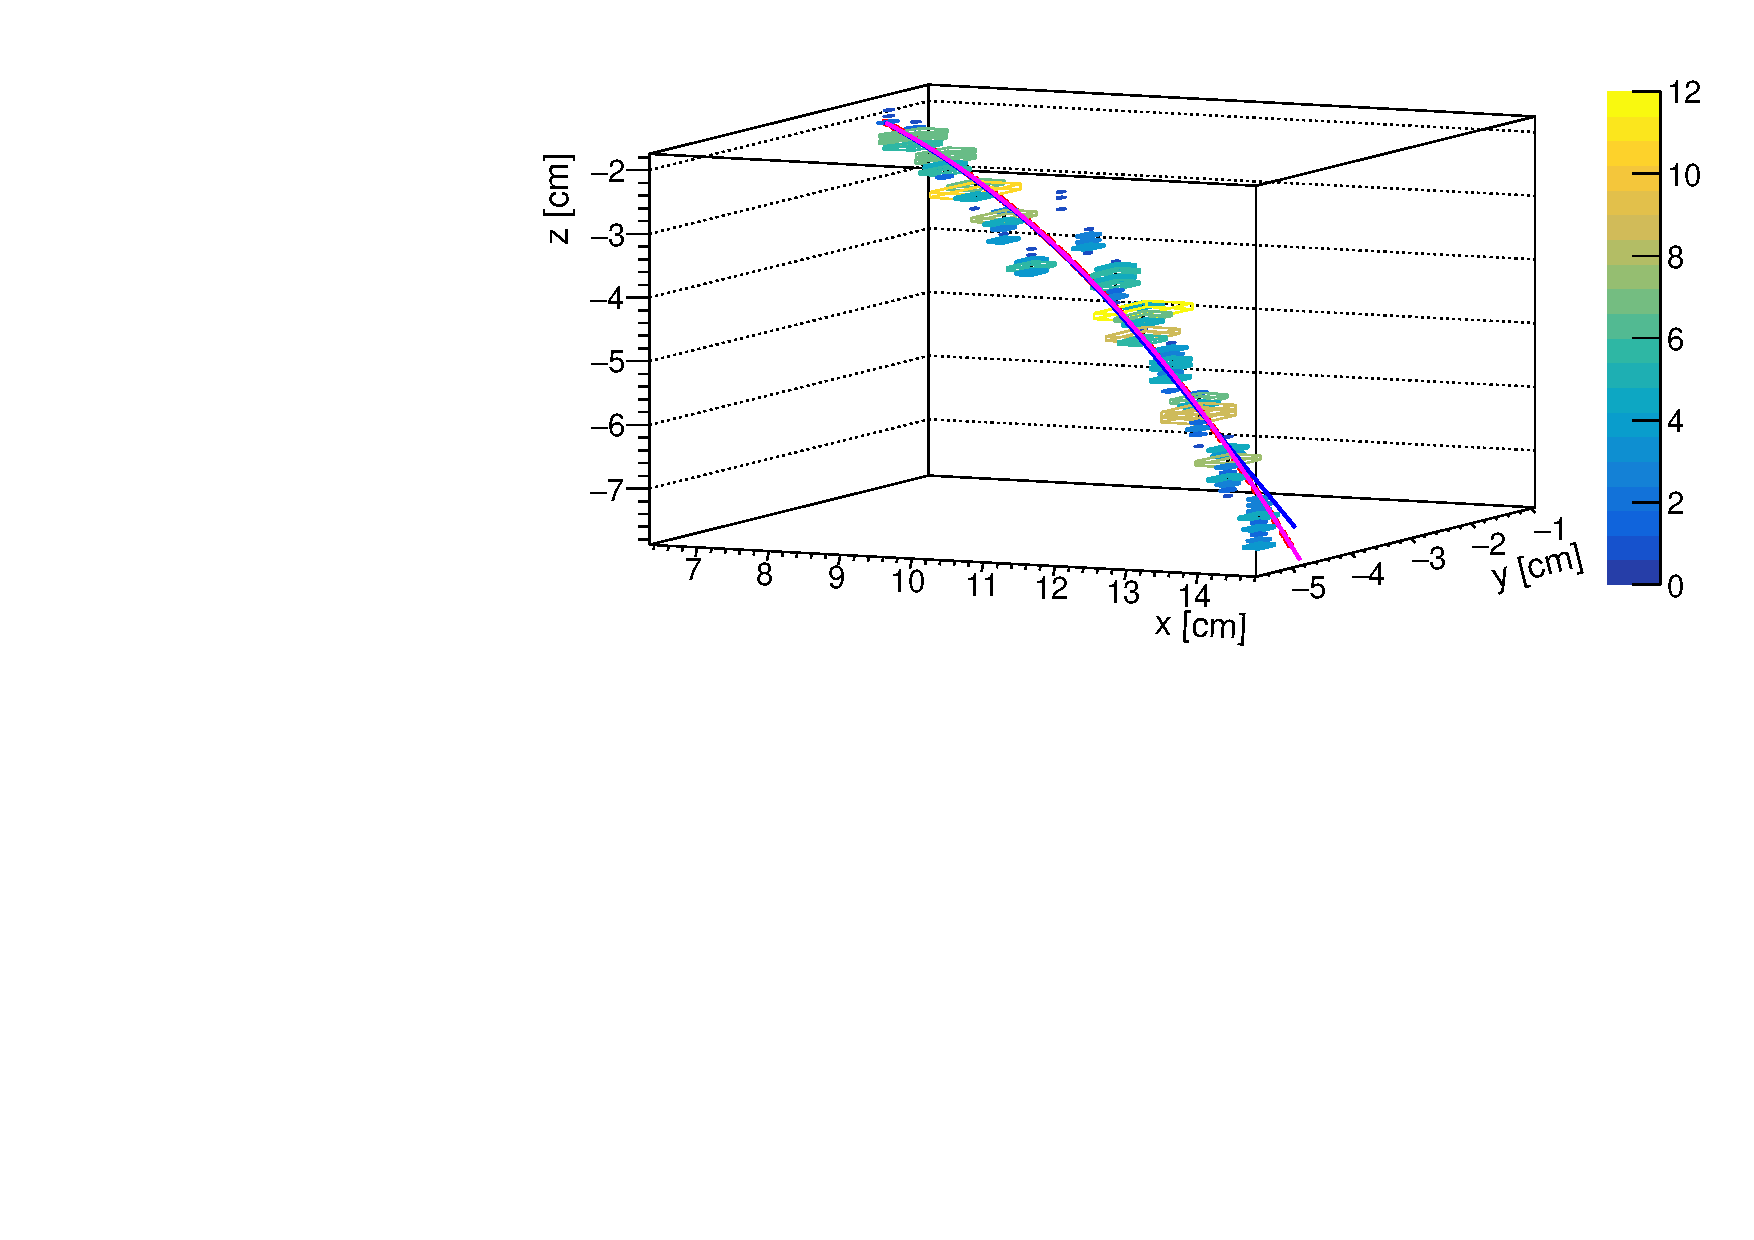
\includegraphics[width=0.85\textwidth]{../../figures/track_rkfit_example.pdf}\\
	\end{frame}
	}
	{\nologo\nonav
	\begin{frame}
		\frametitle{Energy Reconstruction Precision (overall)}
		\centering
		\begin{columns}
			\column{0.5\textwidth}
			\centering
			\Large \textbf{Electrons}
			\vspace{-0.5em}
			\begin{figure}
				\centering
				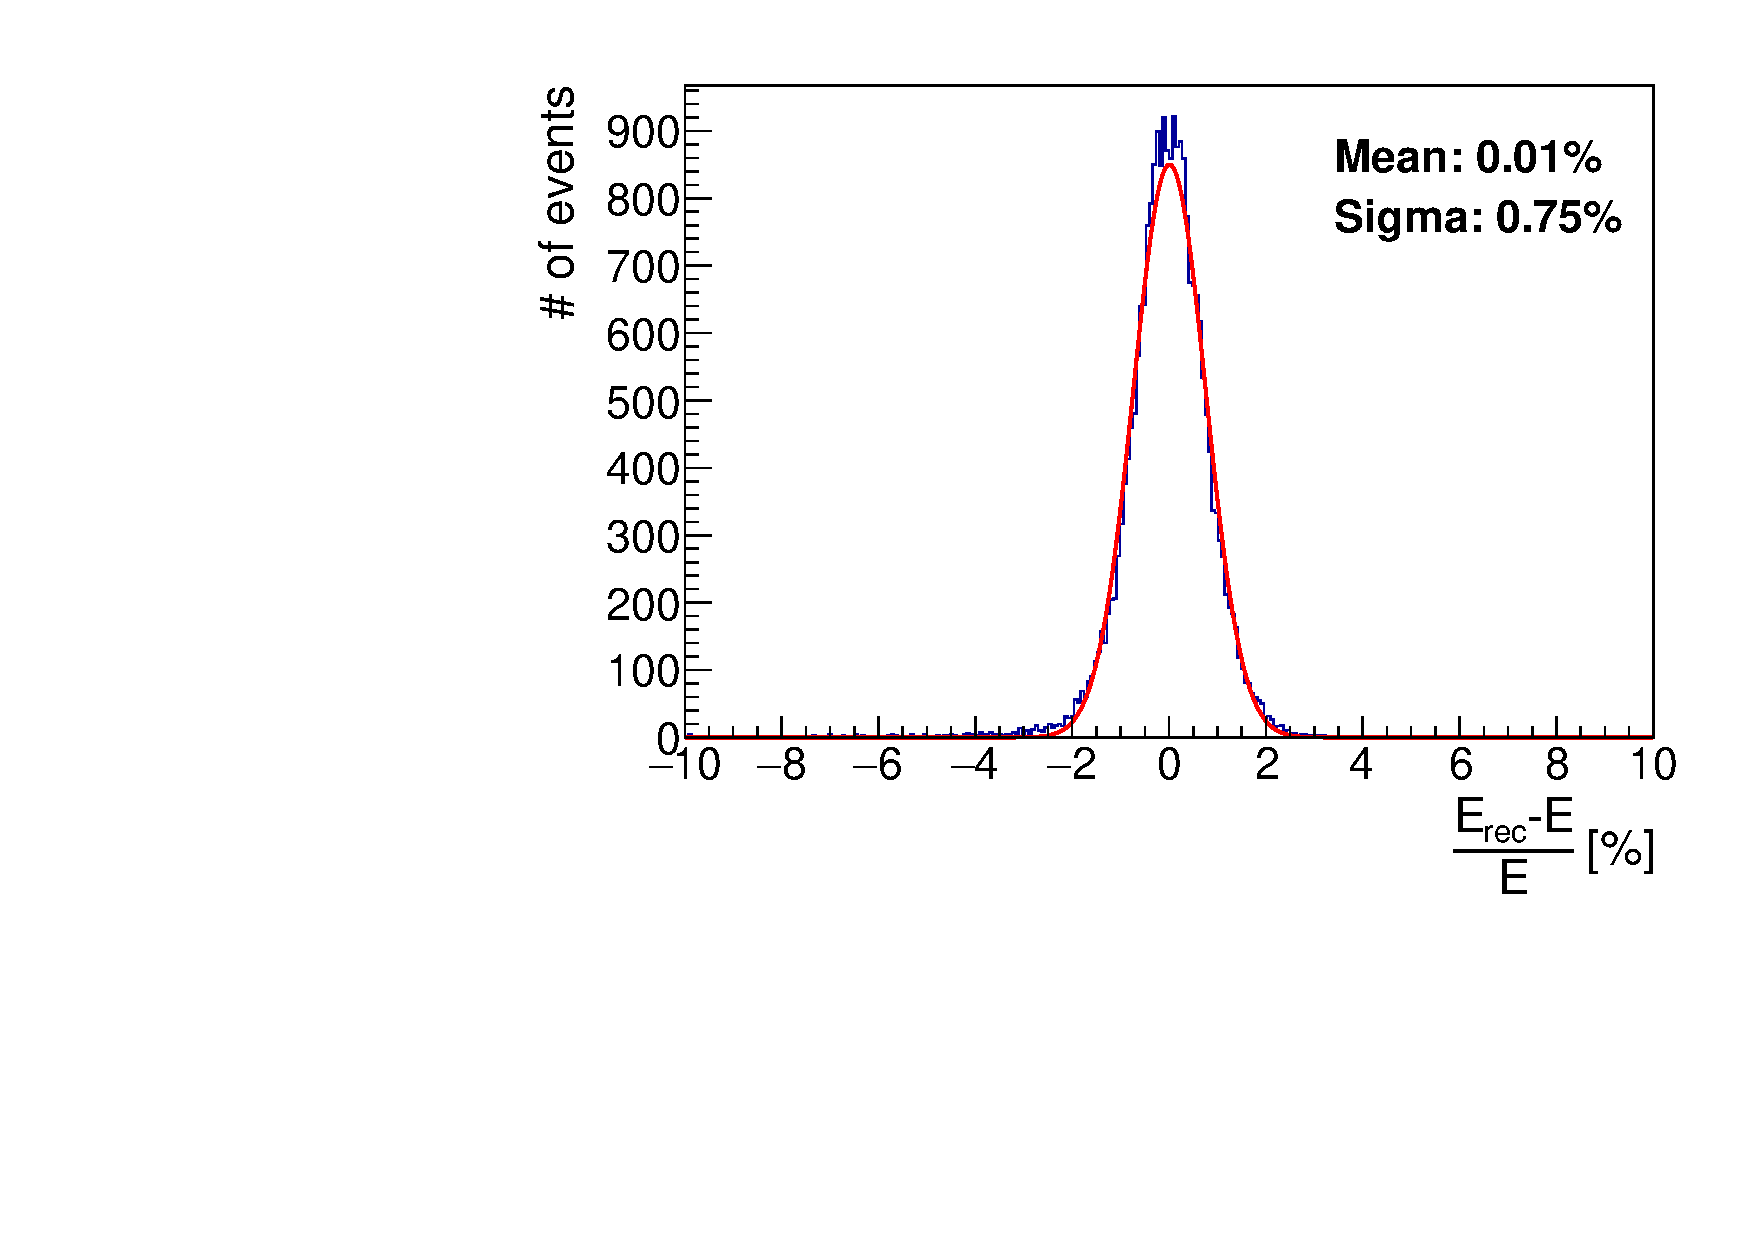
\includegraphics[width = 0.84 \linewidth]{../../figures/c_e_delta_energy_lin.pdf}\\
				%\vspace{-0.2em}
				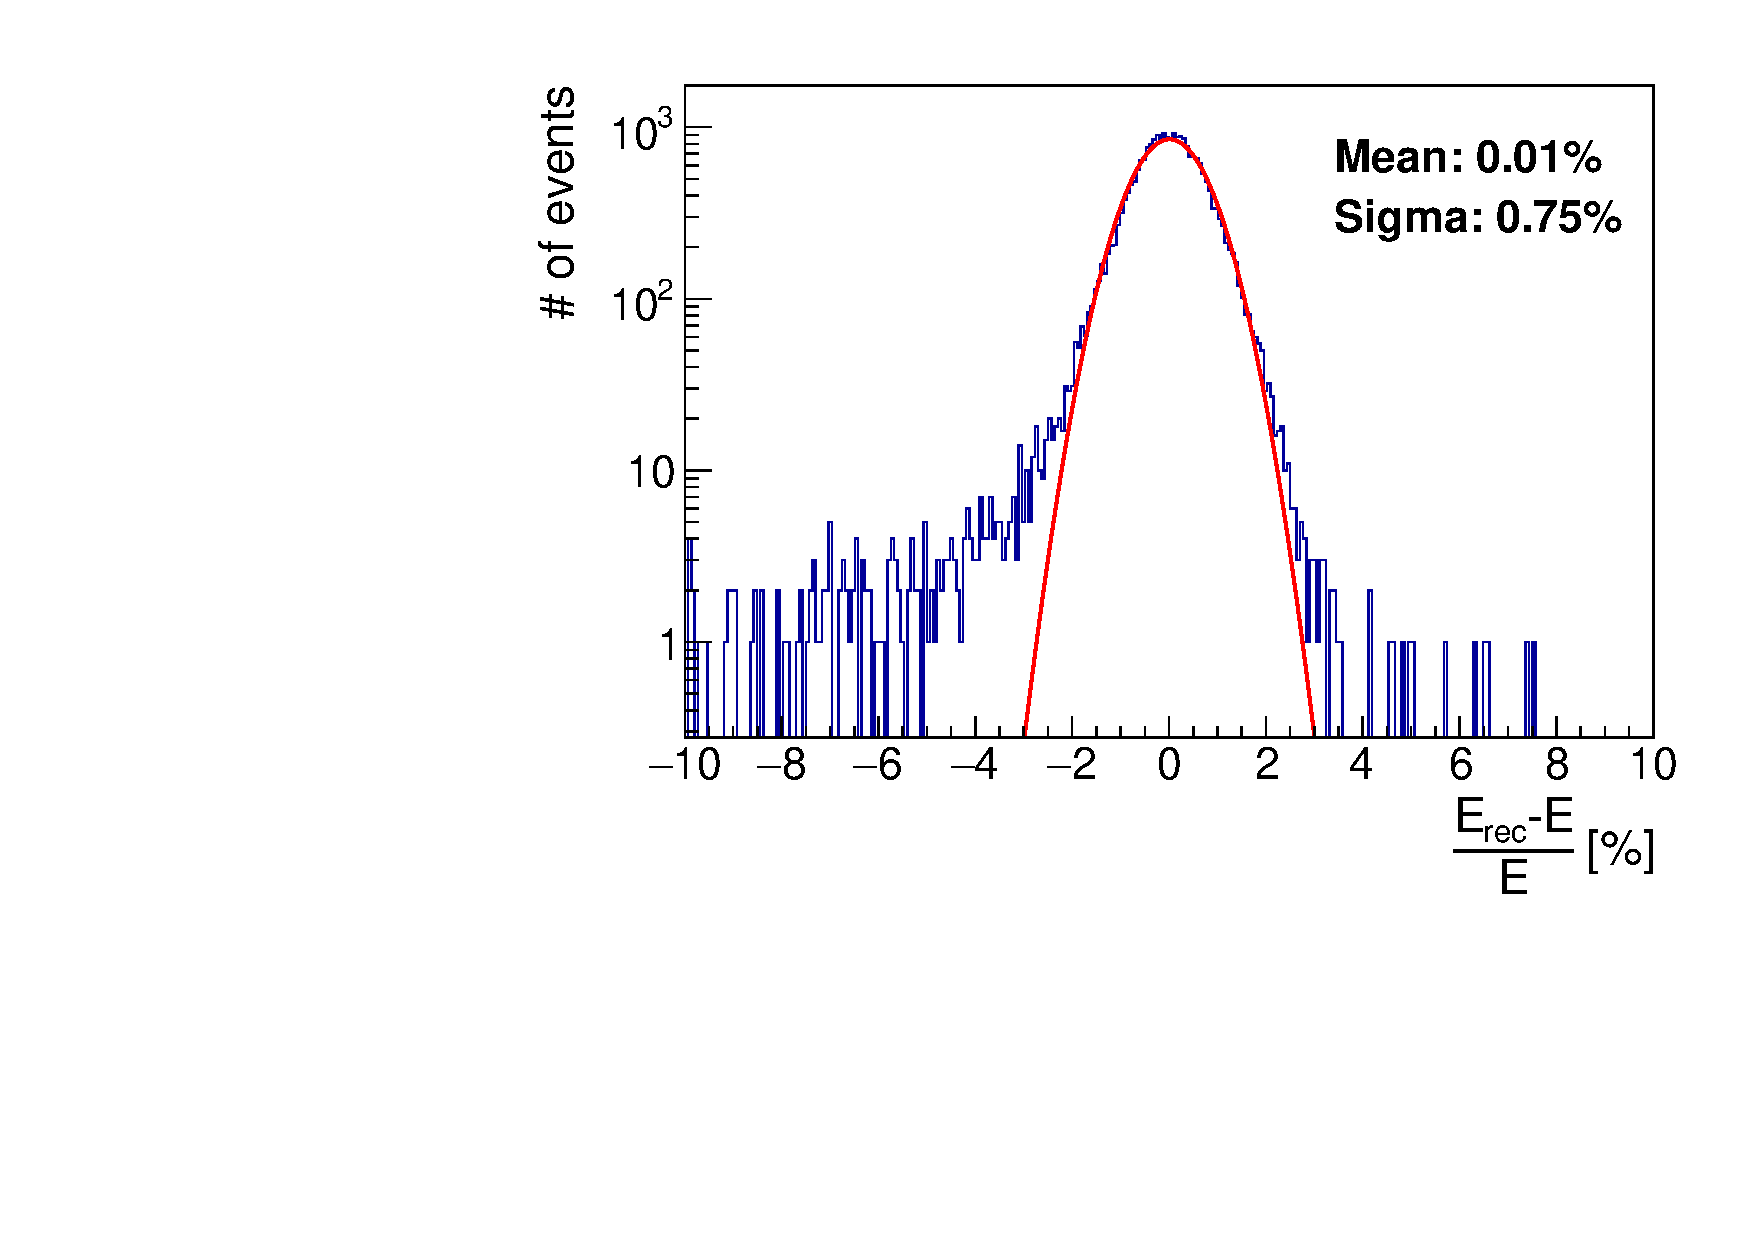
\includegraphics[width = 0.74 \linewidth]{../../figures/c_e_delta_energy_log.pdf}
			\end{figure}
			\column{0.5\textwidth}
			\centering
			\Large \textbf{Positrons}
			\vspace{-0.5em}
			\begin{figure}
				\centering
				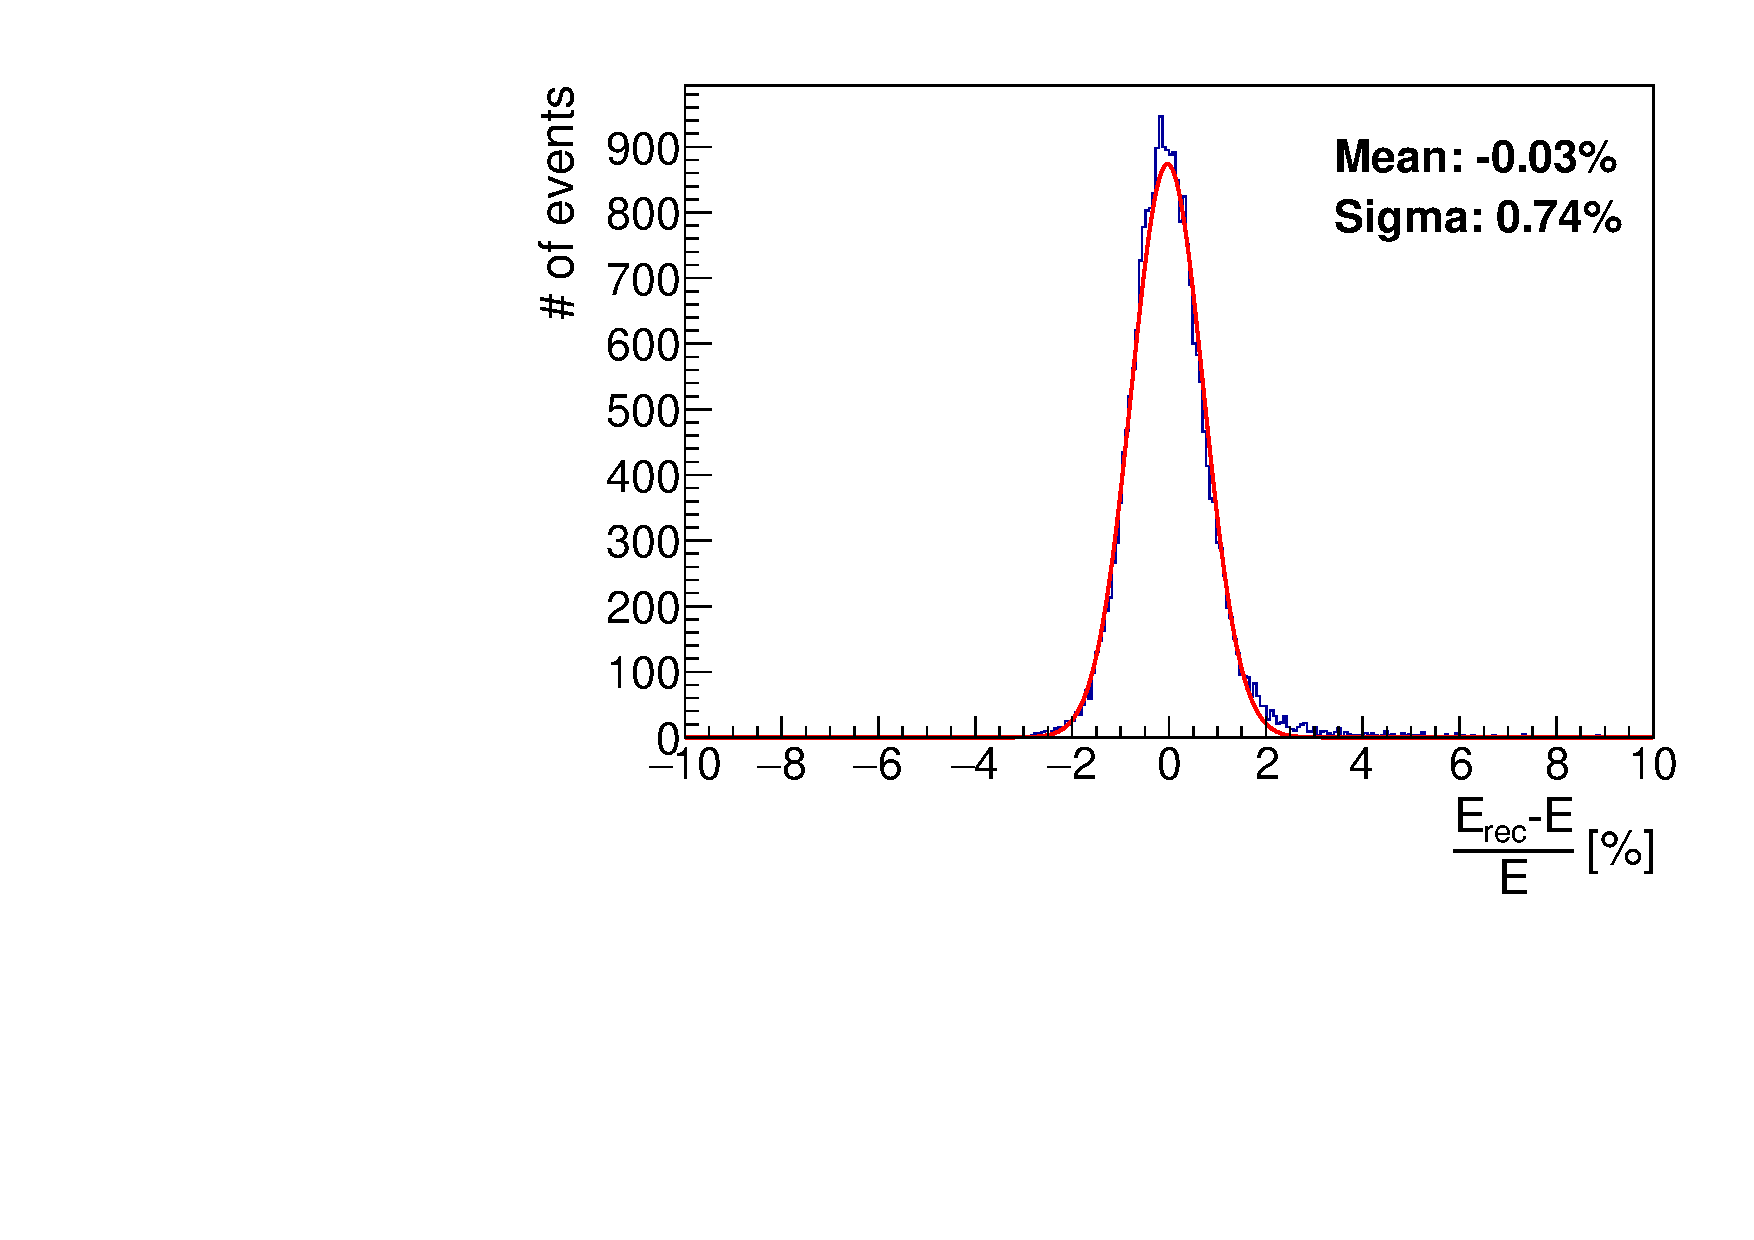
\includegraphics[width = 0.84 \linewidth]{../../figures/c_p_delta_energy_lin.pdf}\\
				%\vspace{-0.2em}
				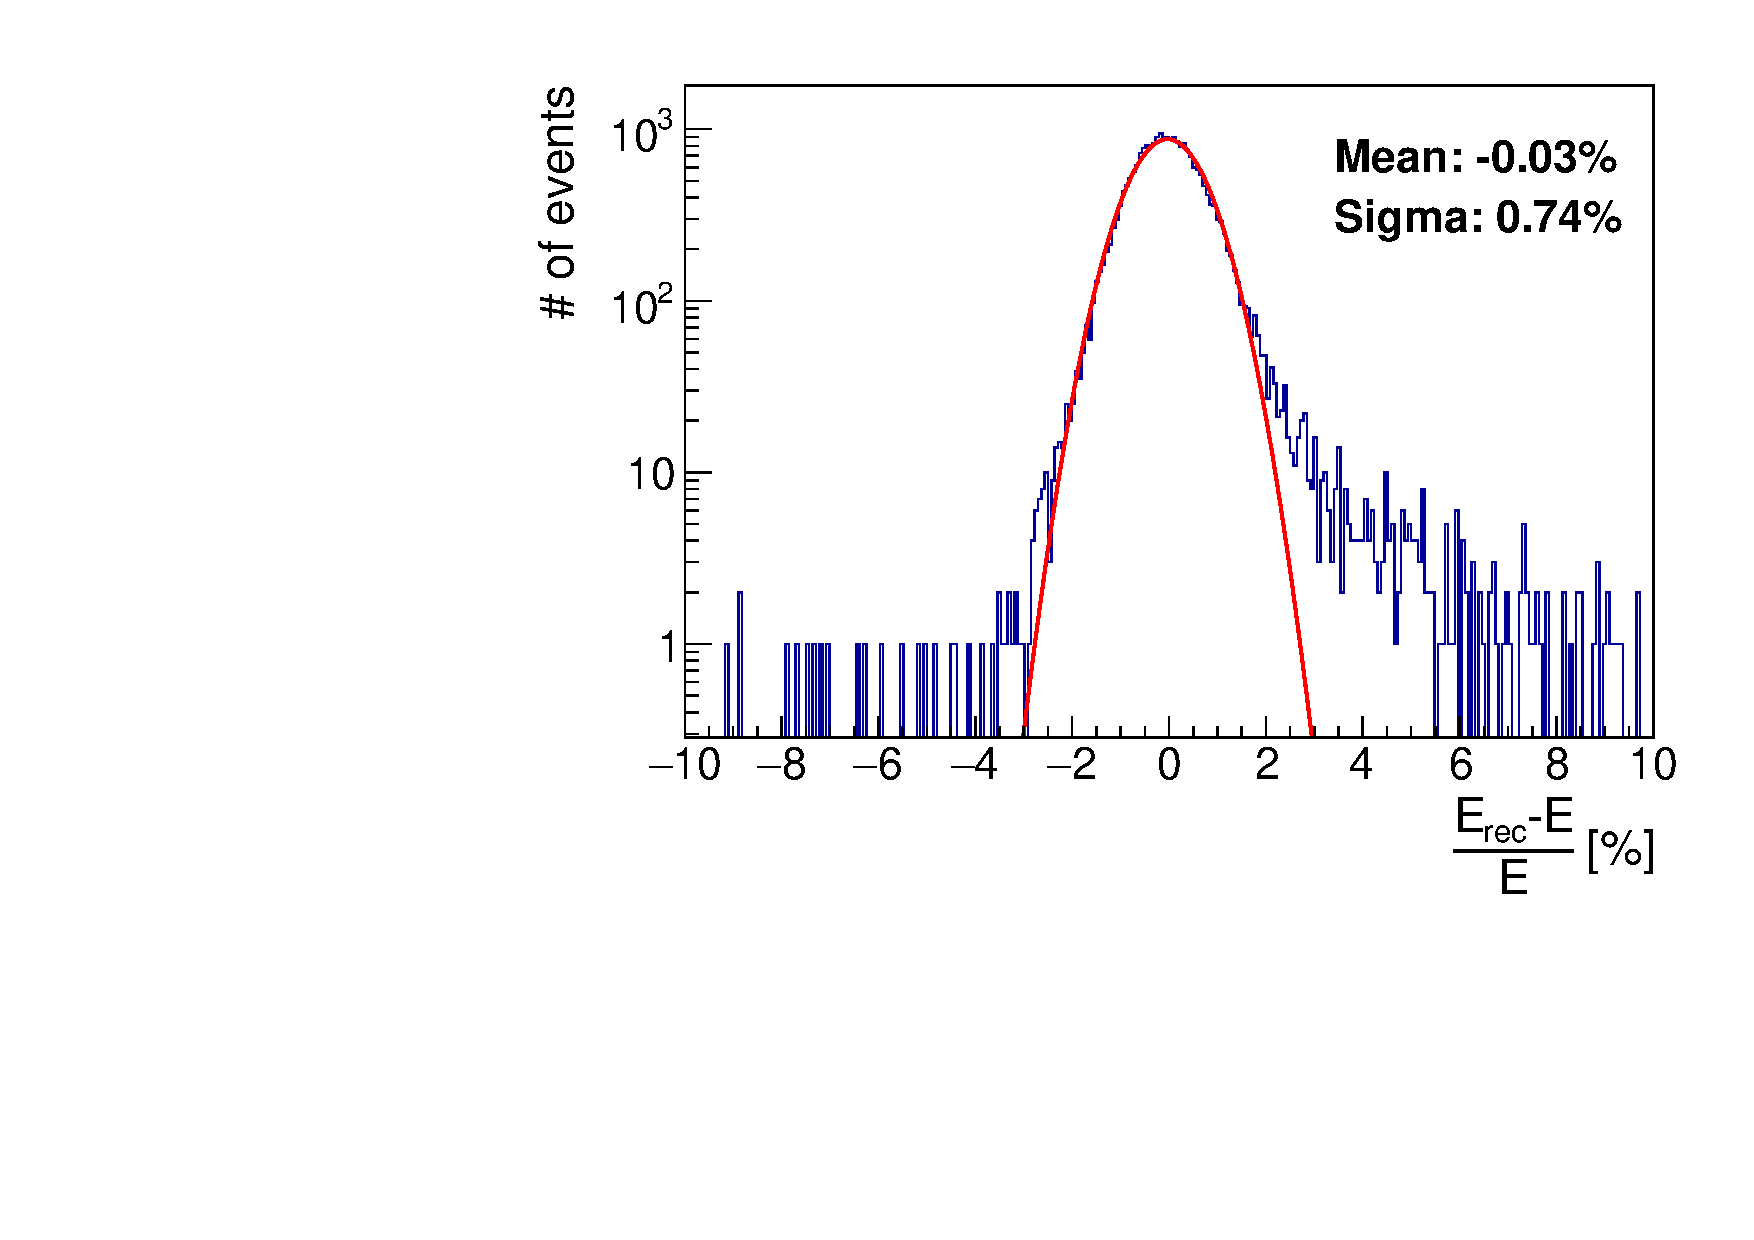
\includegraphics[width = 0.74 \linewidth]{../../figures/c_p_delta_energy_log.pdf}
			\end{figure}
		\end{columns}
		\footnotesize{Relative reconstruction deviation of the~kinetic energy of electron and positron tracks (ca. 24\,000 of each simulated).}
	\end{frame}
	}
	{\nologo
	\begin{frame}
		\frametitle{Effect of multiple scattering (preliminary)}
		\begin{itemize}
			\item Preliminary tests show significant impact of multiple scattering on the resolution.
			\begin{itemize}
				\item Reconstruction of electron tracks with zero $\theta, \varphi$ and total energy 3, 8 and 13~MeV.
				\item Simulation of the full parameter grid is being prepared.
			\end{itemize}
			\item Delta electrons not taken into account for better comparison with previous simulations.
			\item Initial position and orientation still fixed in the fit (might increase the error).
		\end{itemize}
		
		\begin{columns}
			\column{0.33\textwidth}
			\centering
			\large \textbf{3 MeV}
			\vspace{-0.33cm}
			\begin{figure}
				\centering
				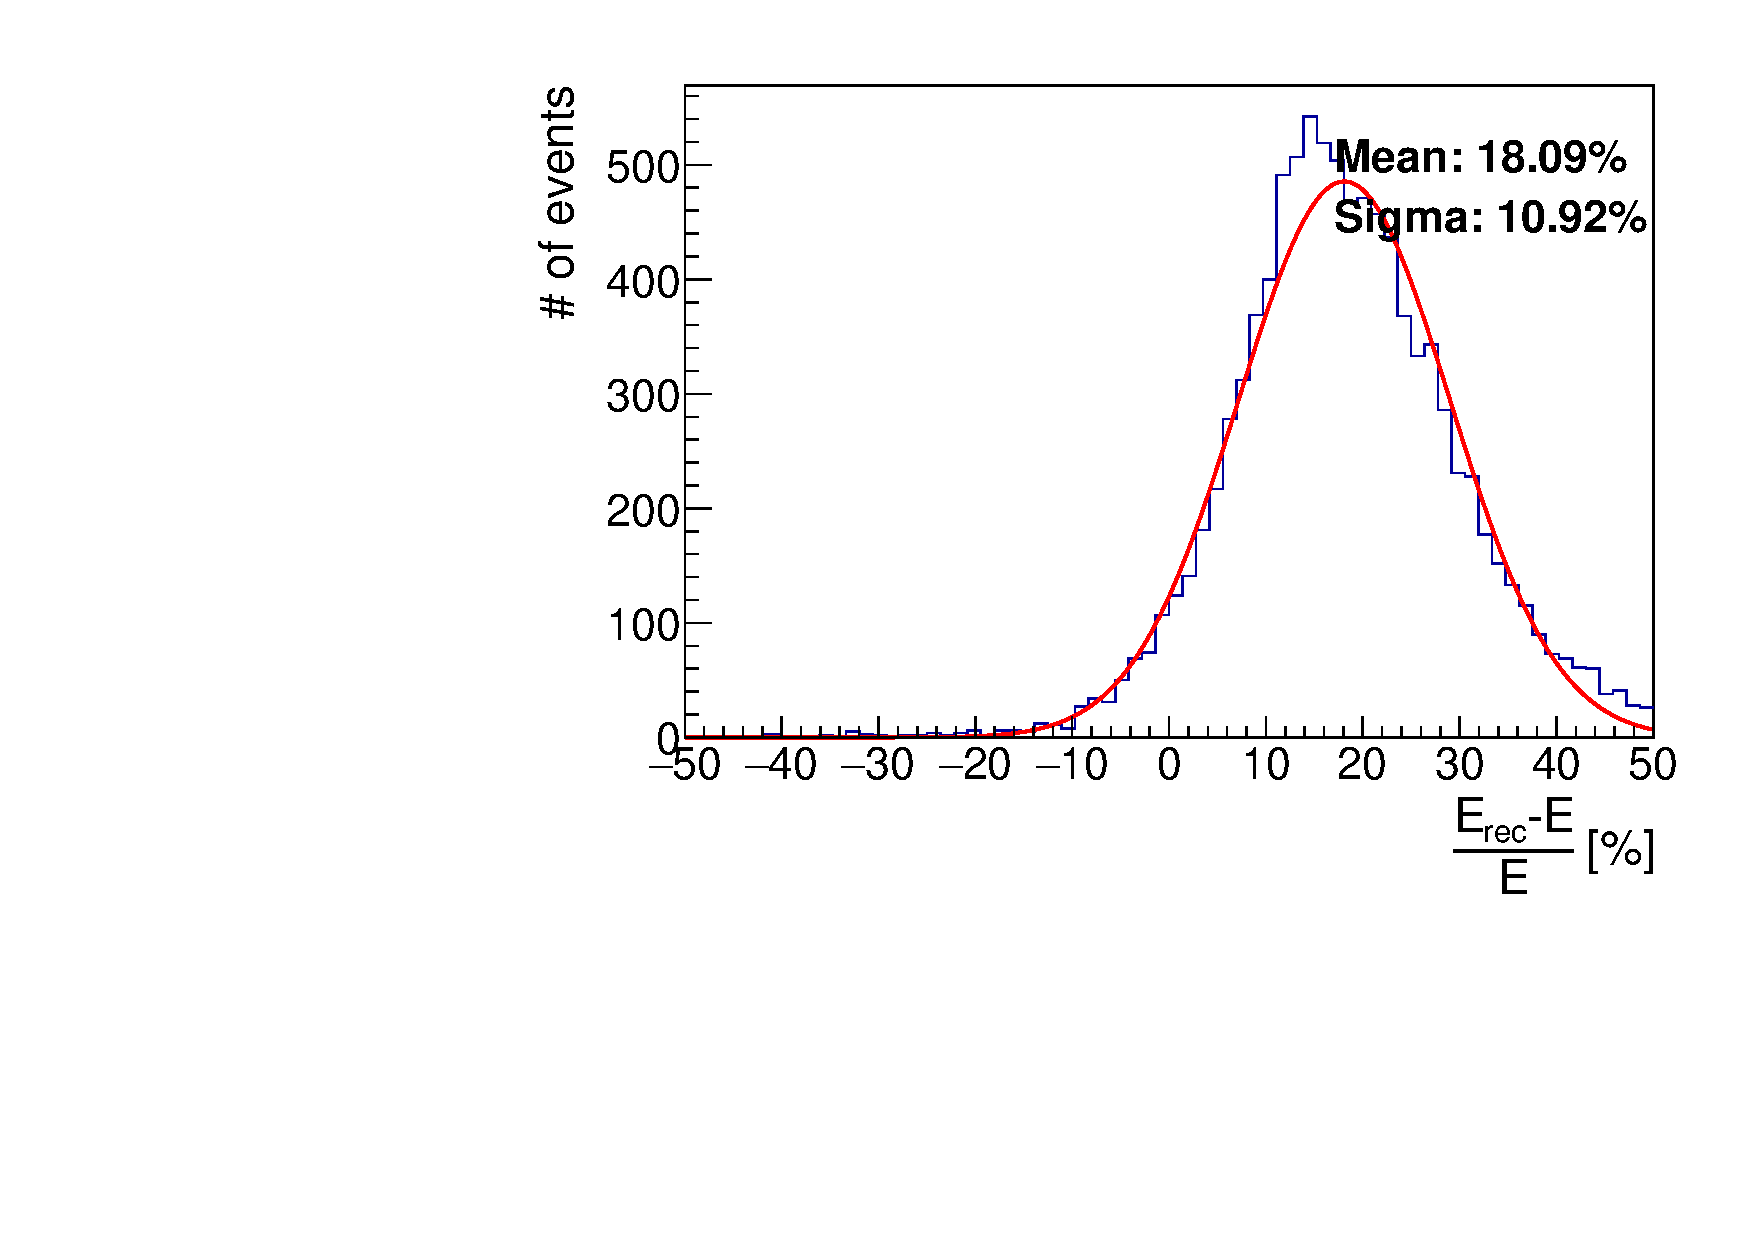
\includegraphics[width = 0.85 \linewidth]{../../figures/mcs_3MeV.pdf}
			\end{figure}
			\column{0.33\textwidth}
			\centering
			\large \textbf{8 MeV}
			\vspace{-0.33cm}
			\begin{figure}
				\centering
				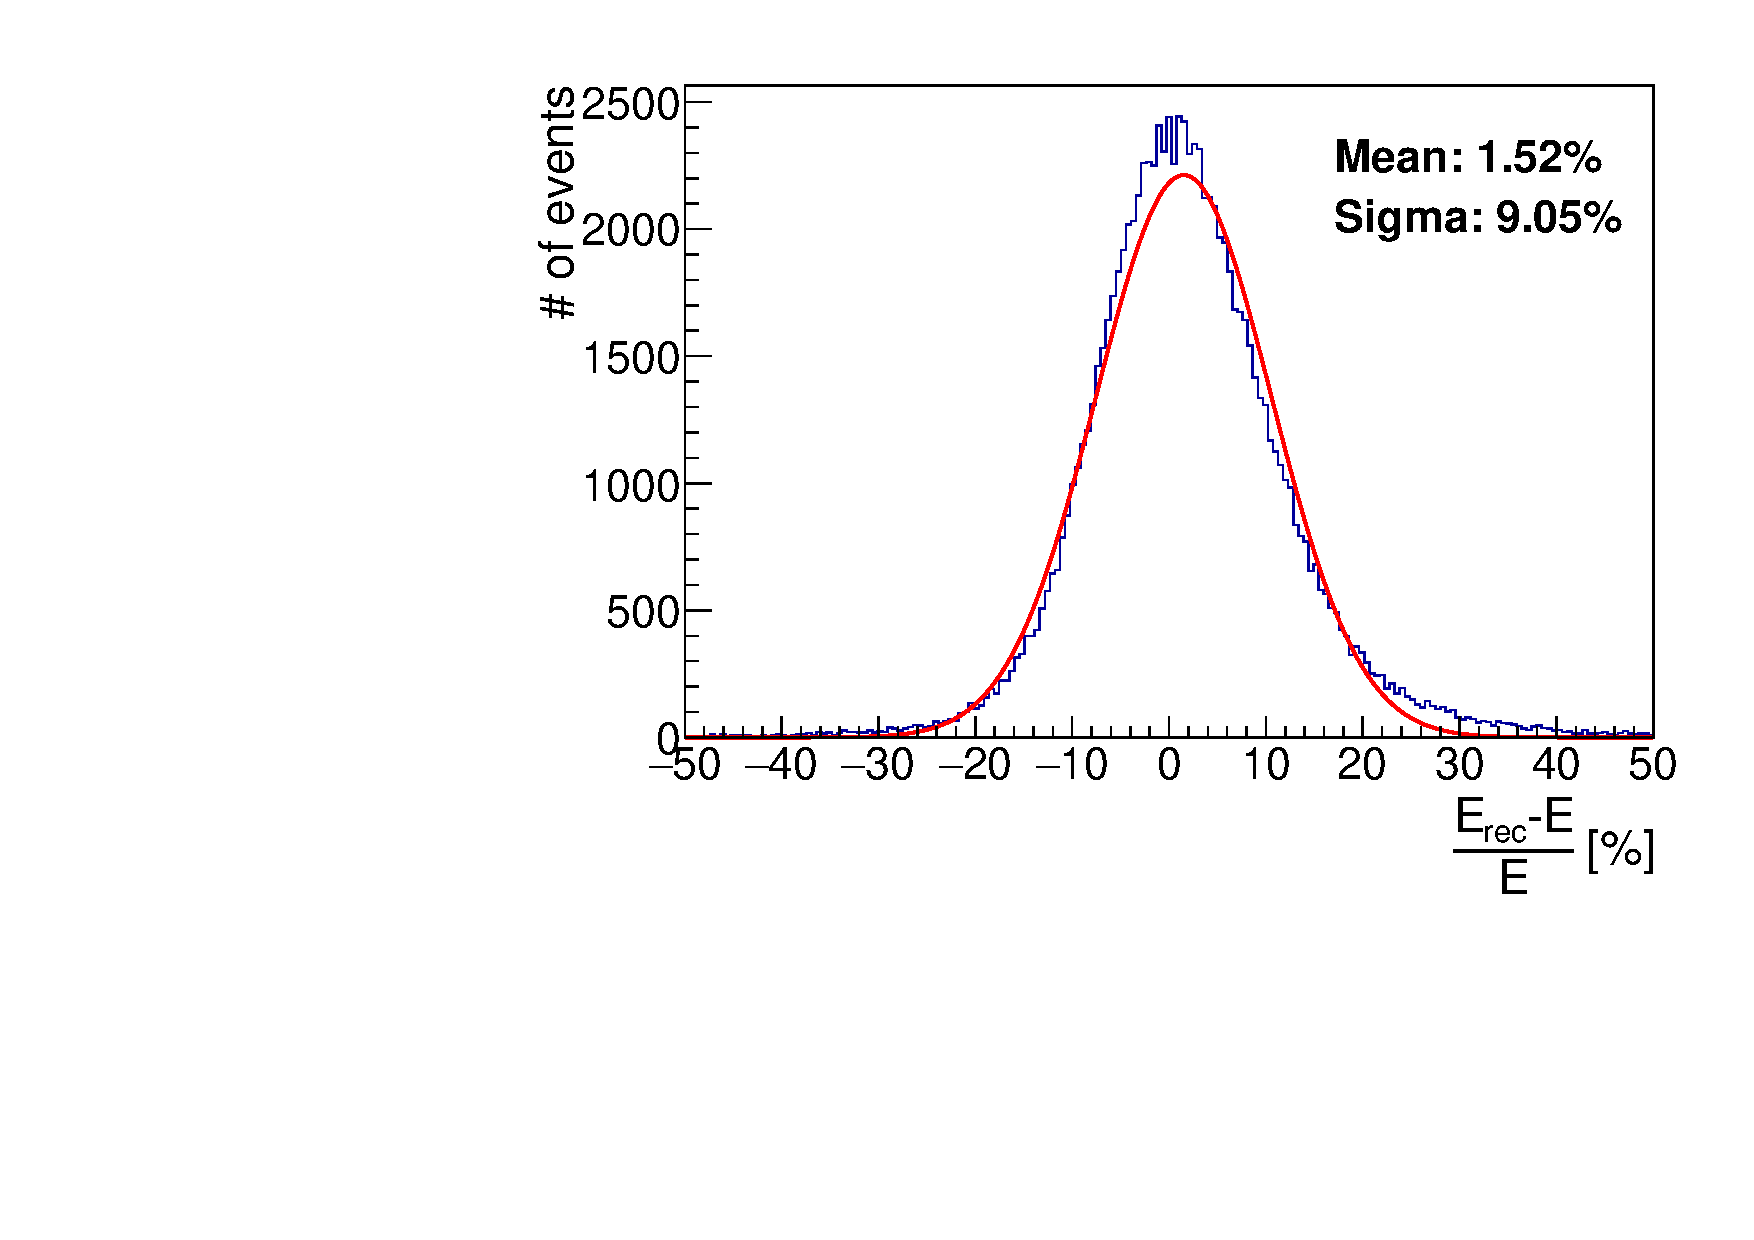
\includegraphics[width = 0.85 \linewidth]{../../figures/mcs_8MeV.pdf}
			\end{figure}
			\column{0.33\textwidth}
			\centering
			\large \textbf{13 MeV}
			\vspace{-0.33cm}
			\begin{figure}
				\centering
				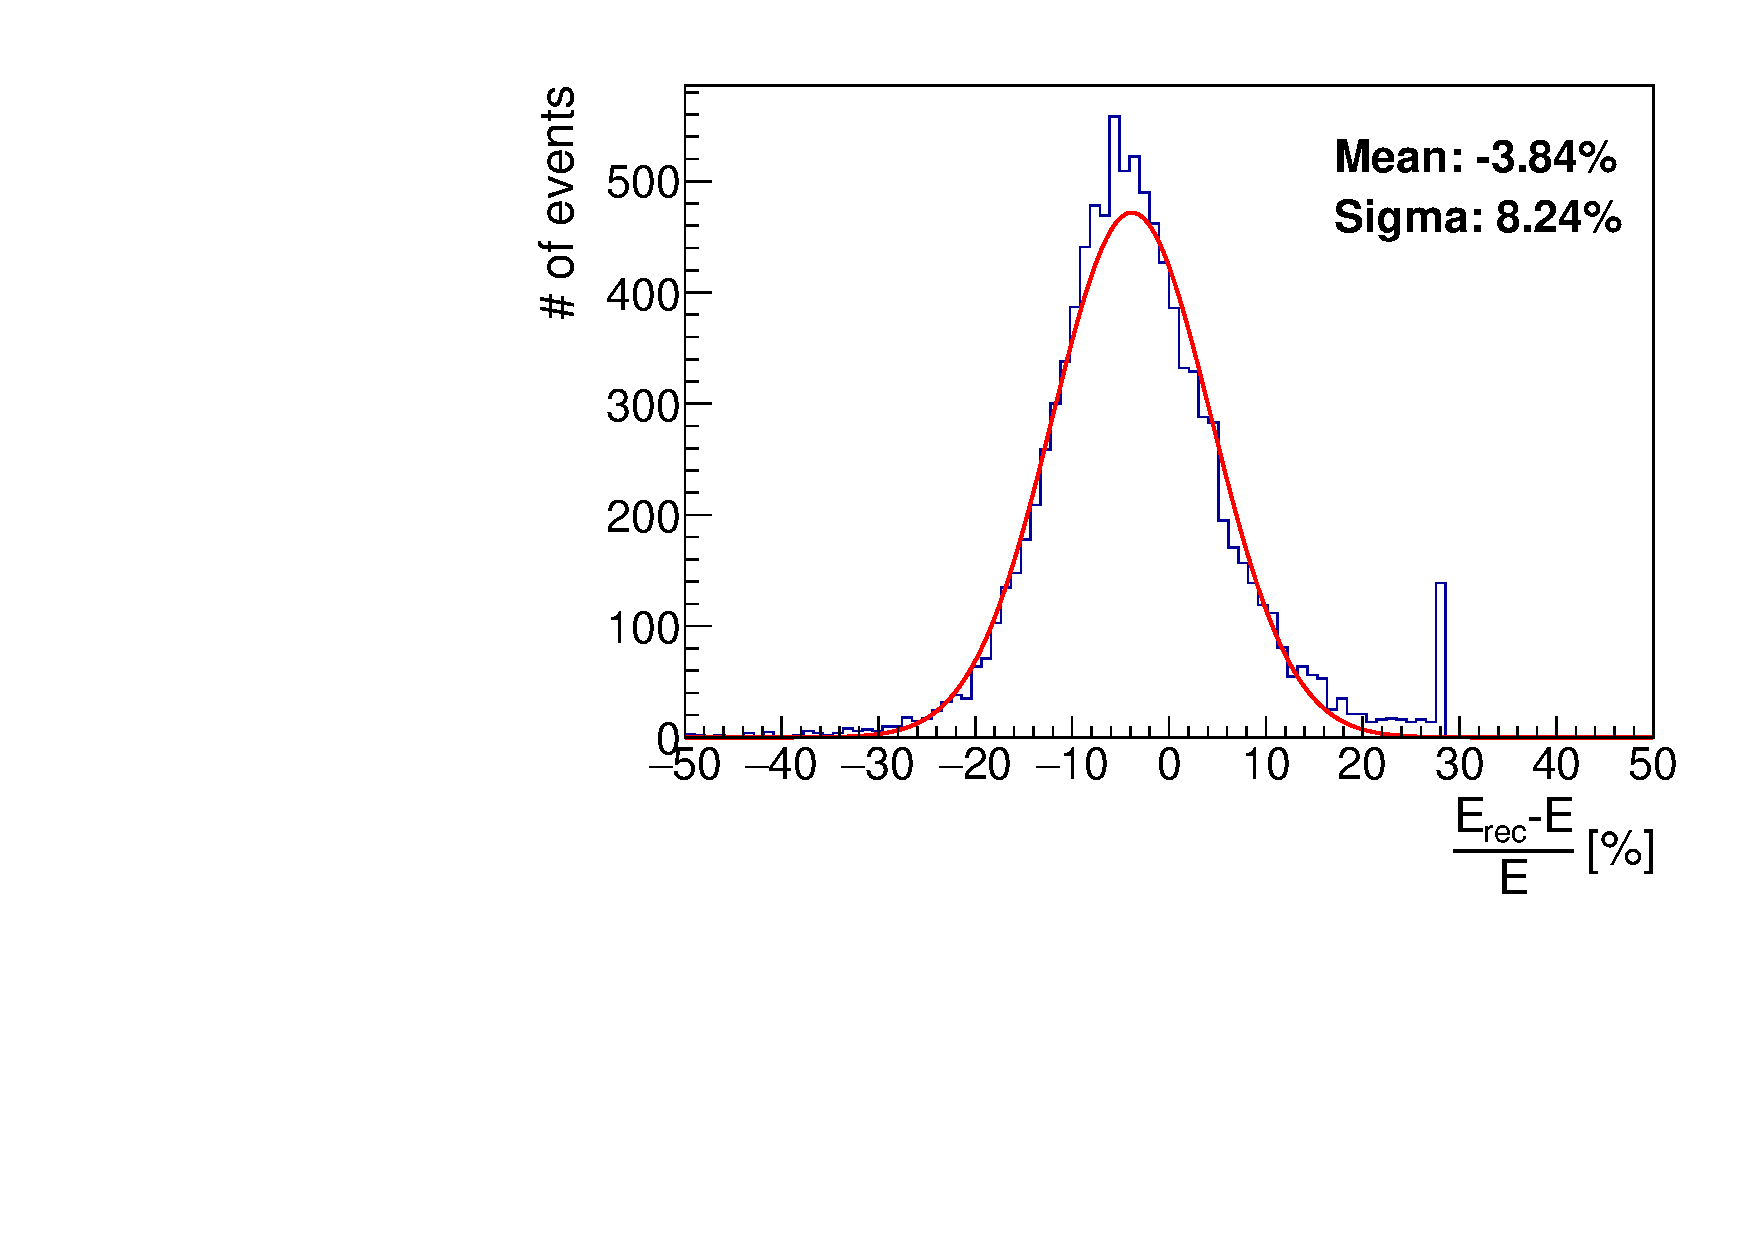
\includegraphics[width = 0.85 \linewidth]{../../figures/mcs_13MeV.pdf}
			\end{figure}
		\end{columns}
	\end{frame}
	}

	\section{Summary}	
	\begin{frame}
		\frametitle{Summary}
		\begin{itemize}
			\item Several batches of tracks have been simulated for testing purposes.
			\begin{itemize}
				\item $\theta\in[-17.1^\circ,17.1^\circ]$, $\varphi~\in~[-16.3^\circ,16.3^\circ]$, $ E_k \in [3,13] $~MeV
			\end{itemize}
			\item The map of ionization electron readout positions and drift times has been generated.
			\item The map has been tested by the track reconstruction.
			\item Some of the systematic errors were corrected.
			\item The results suggest that:
			\begin{itemize}
				\item Current energy resolution (fitted sigma) is 0.75~\% for electrons and positrons under idealized conditions.
				\item Multiple scattering is expected to reduce it significantly (up to \textapprox 11~\% for low energies), further investigation is needed.
				\item OFTPC works well on a simulation level.
			\end{itemize}
		\end{itemize}
	\end{frame}
	
	{
		%\usebackgroundtemplate{\includegraphics[width=\paperwidth,height=\paperheight]{../images/DSC_5602.jpg}}%
		\begin{frame}[noframenumbering]{}
			\begin{center}
				\Huge Thank you for your attention.
			\end{center}
		\end{frame}
	}
	
	%\section{References}
	\begin{frame}[allowframebreaks,noframenumbering]
		\frametitle{References}
		\printbibliography
		%\bibliography{references}
		%\bibliographystyle{unsrt}
	\end{frame}
	
	\begin{frame}[noframenumbering]{}
		\begin{center}
			\Huge Backup
		\end{center}
	\end{frame}
	
	\appendix
	%\setcounter{framenumber}{0}
	\renewcommand{\insertframenumber}{B\arabic{framenumber}}
	
	\begin{frame}
		\frametitle{Track Simulation: Parameters}
		\centering
		\large{Spherical angles ($\theta$,$\varphi$) with respect to~$z$}\\
		\small{$\theta$ taken from the equatorial plane $xy$}
		\centering
		\textcolor{white}{aaaaaaaa}\includegraphics[height= 0.61 \textheight]{figures/tpc_ggb.png}\newline
		\small{Diagram of the batch simulation parameters:\\ $\theta\in[-17.1^\circ,17.1^\circ]$, $\varphi~\in~[-16.3^\circ,16.3^\circ]$, $ E_\text{kin.} \in [3,13] $~MeV.\\}
		\tiny{Made with GeoGebra®.}
	\end{frame}
	
	\begin{frame}
		\frametitle{Track Simulation -- TPC Window}
		\centering
		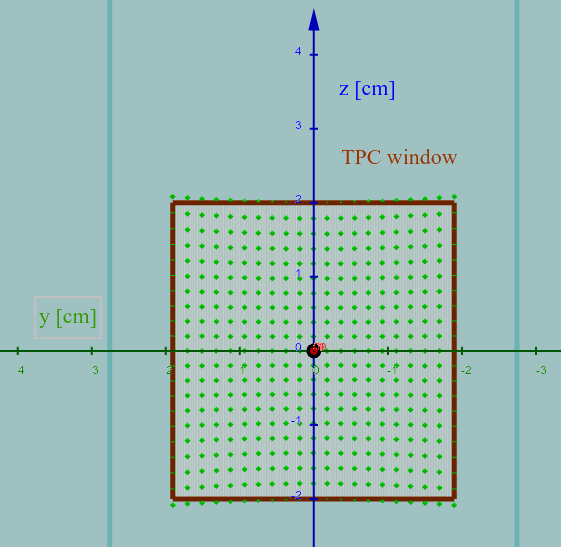
\includegraphics[width=0.6\textwidth]{../images/tpc_window_sim.png}\\
		\vspace{0.5em}
		Initial points of tracks. \tiny{Made with GeoGebra®.}
	\end{frame}
	
	\begin{frame}
		\frametitle{Ionization Electron Map Simulation: Coordinate Distortion}
		\begin{figure}
			\centering
			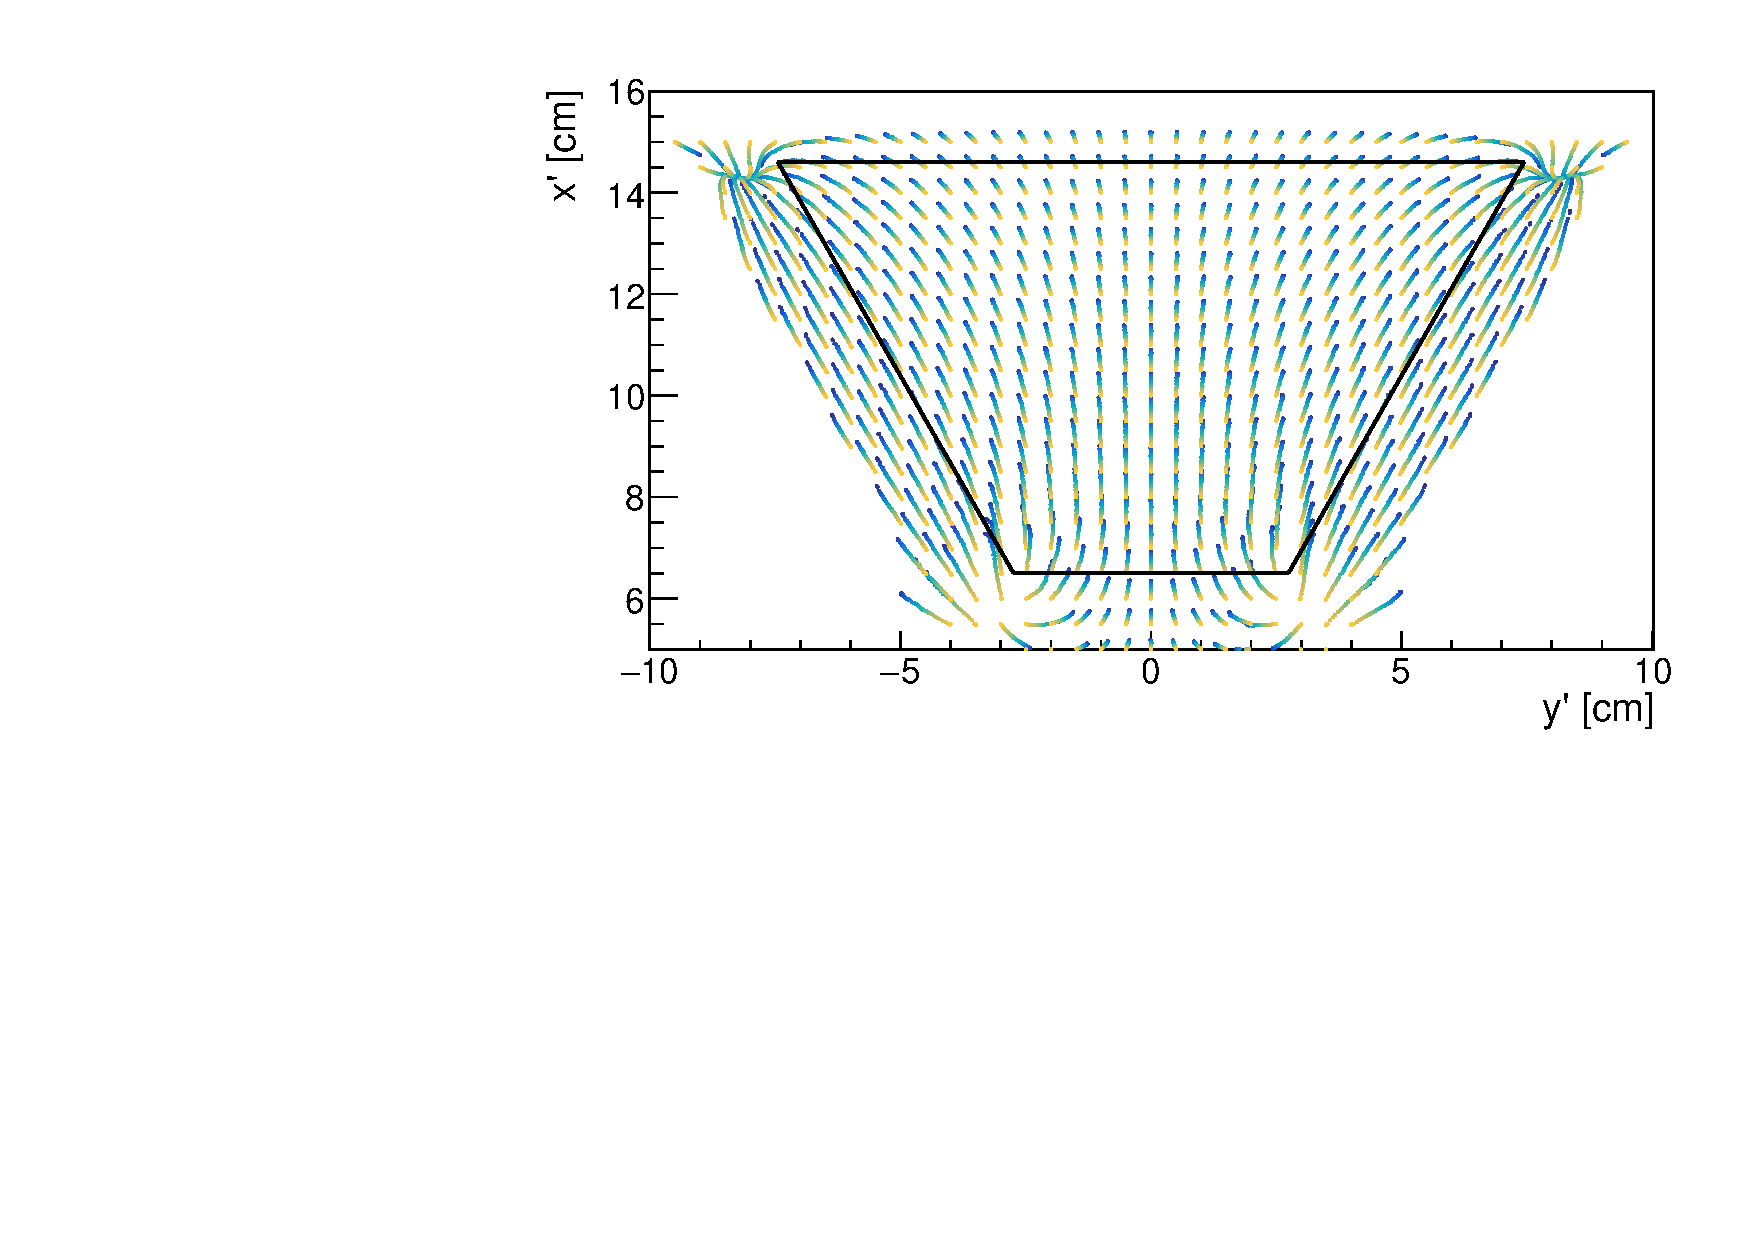
\includegraphics[height=0.68\textheight]{../../figures/map_yx_all.pdf}\\
			\small{$x$ and $y$ coordinate distortion at different $z$ values (denoted by colors).}
		\end{figure}
	\end{frame}
	
	\begin{frame}
		\frametitle{Ionization Electron Map Simulation}
		\centering
		\begin{minipage}[c]{\textwidth}
			\begin{figure}
				\centering
				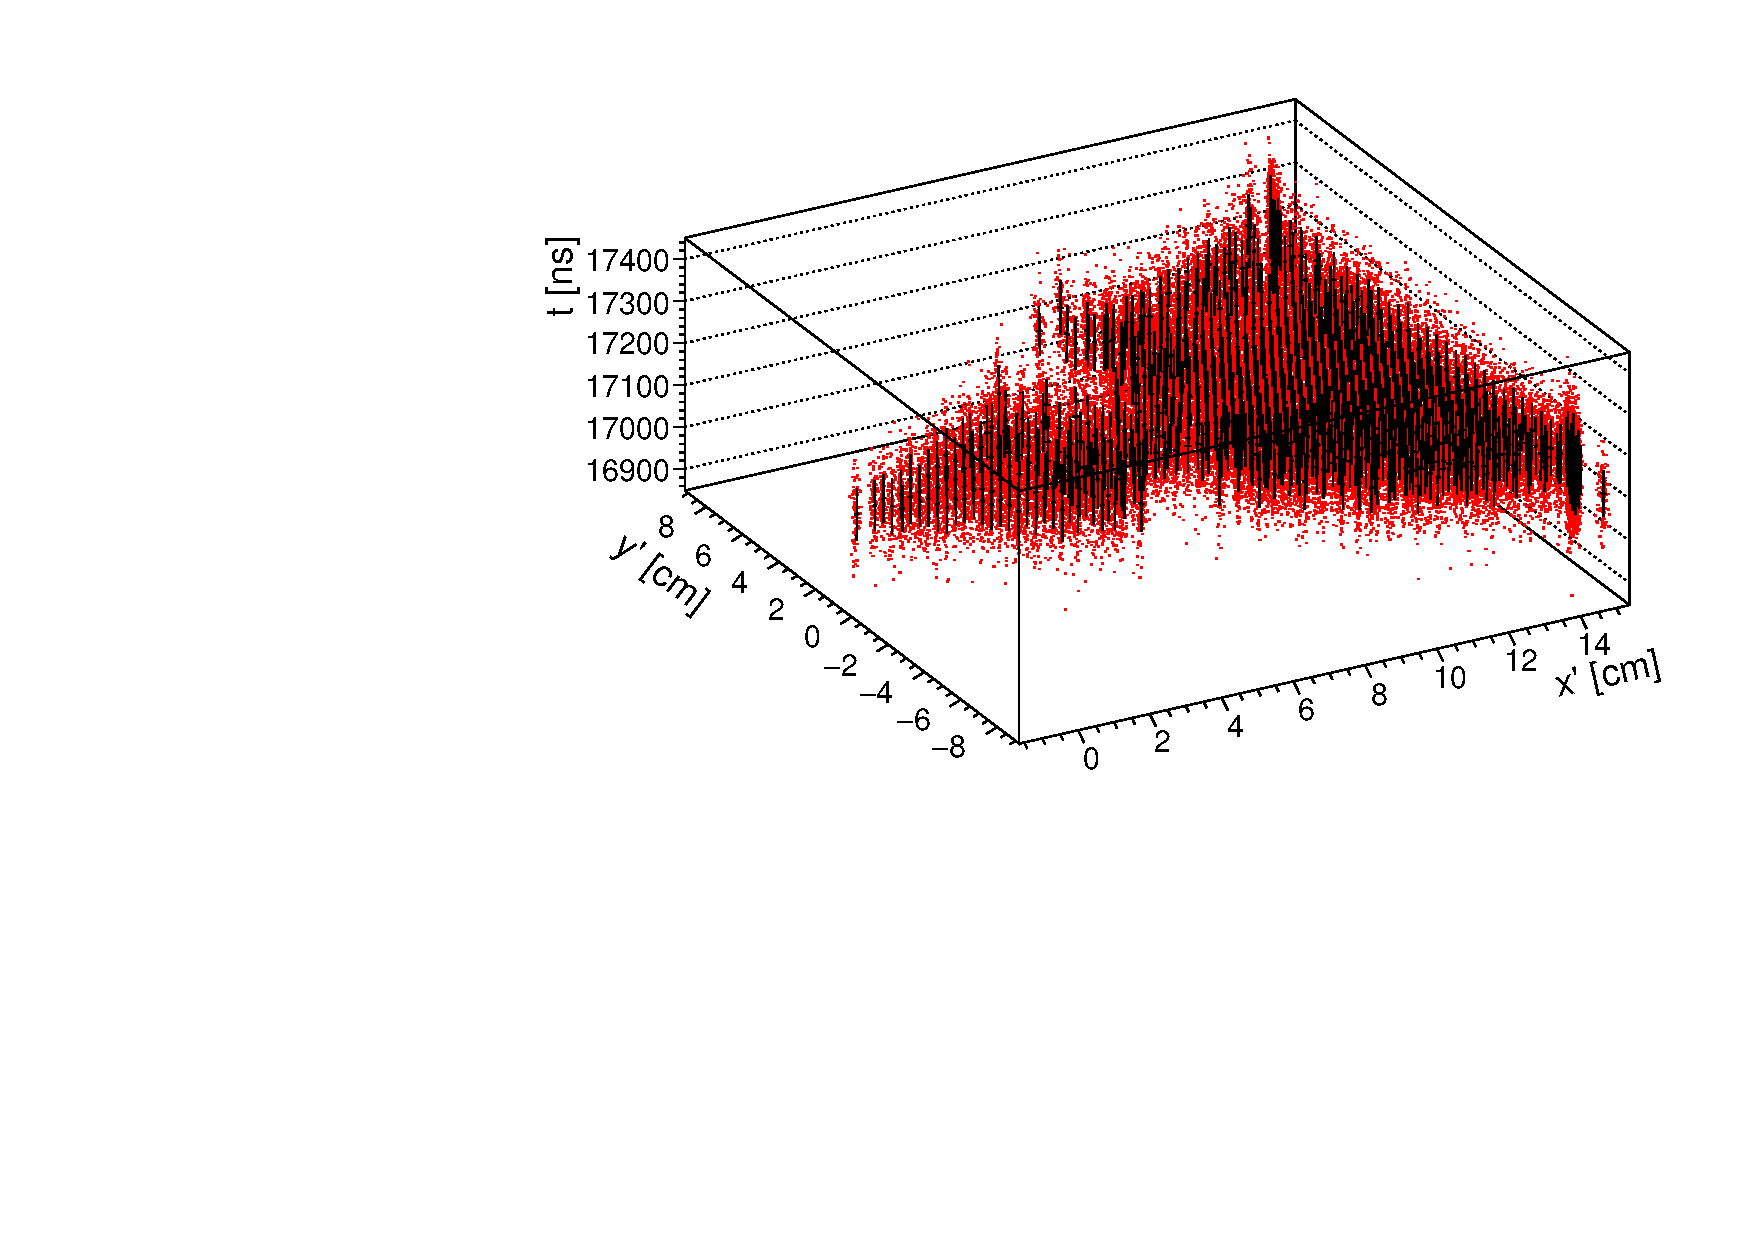
\includegraphics[height=0.7\textheight]{../../figures/map_xyt.pdf}\\
				\small{Mapping of the layer furthest from the OFTPC readout.}
			\end{figure}
		\end{minipage}
	\end{frame}
	
	{\nonav
		\begin{frame}
			\frametitle{Ionization Electron Map Reconstruction Residuals ($x$, $y$)}
			\footnotesize Residuals of init. positions of 14.3 M simul. track ion. $e^-$ reconstructed using the map
			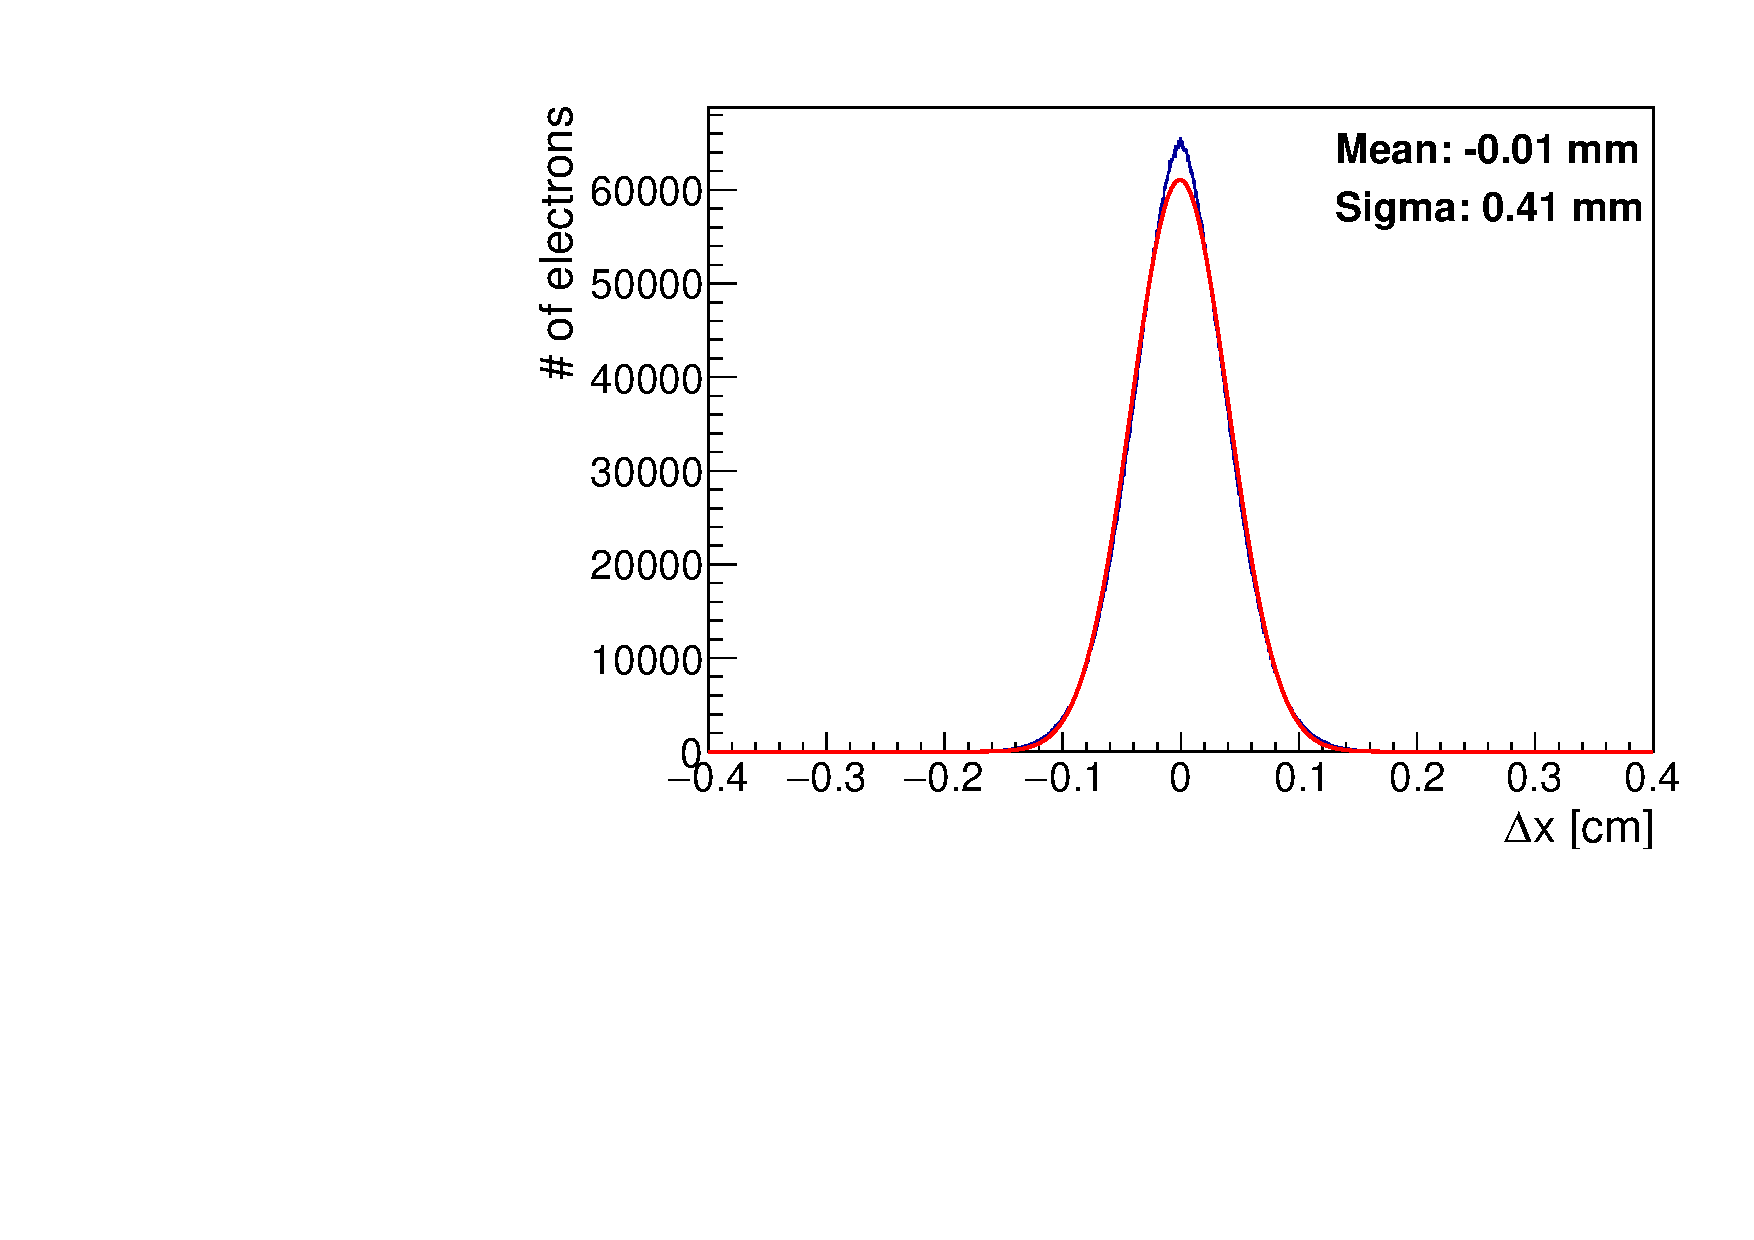
\includegraphics[width=0.45\textwidth]{../../figures/c_fit_res_x_lin.pdf}
			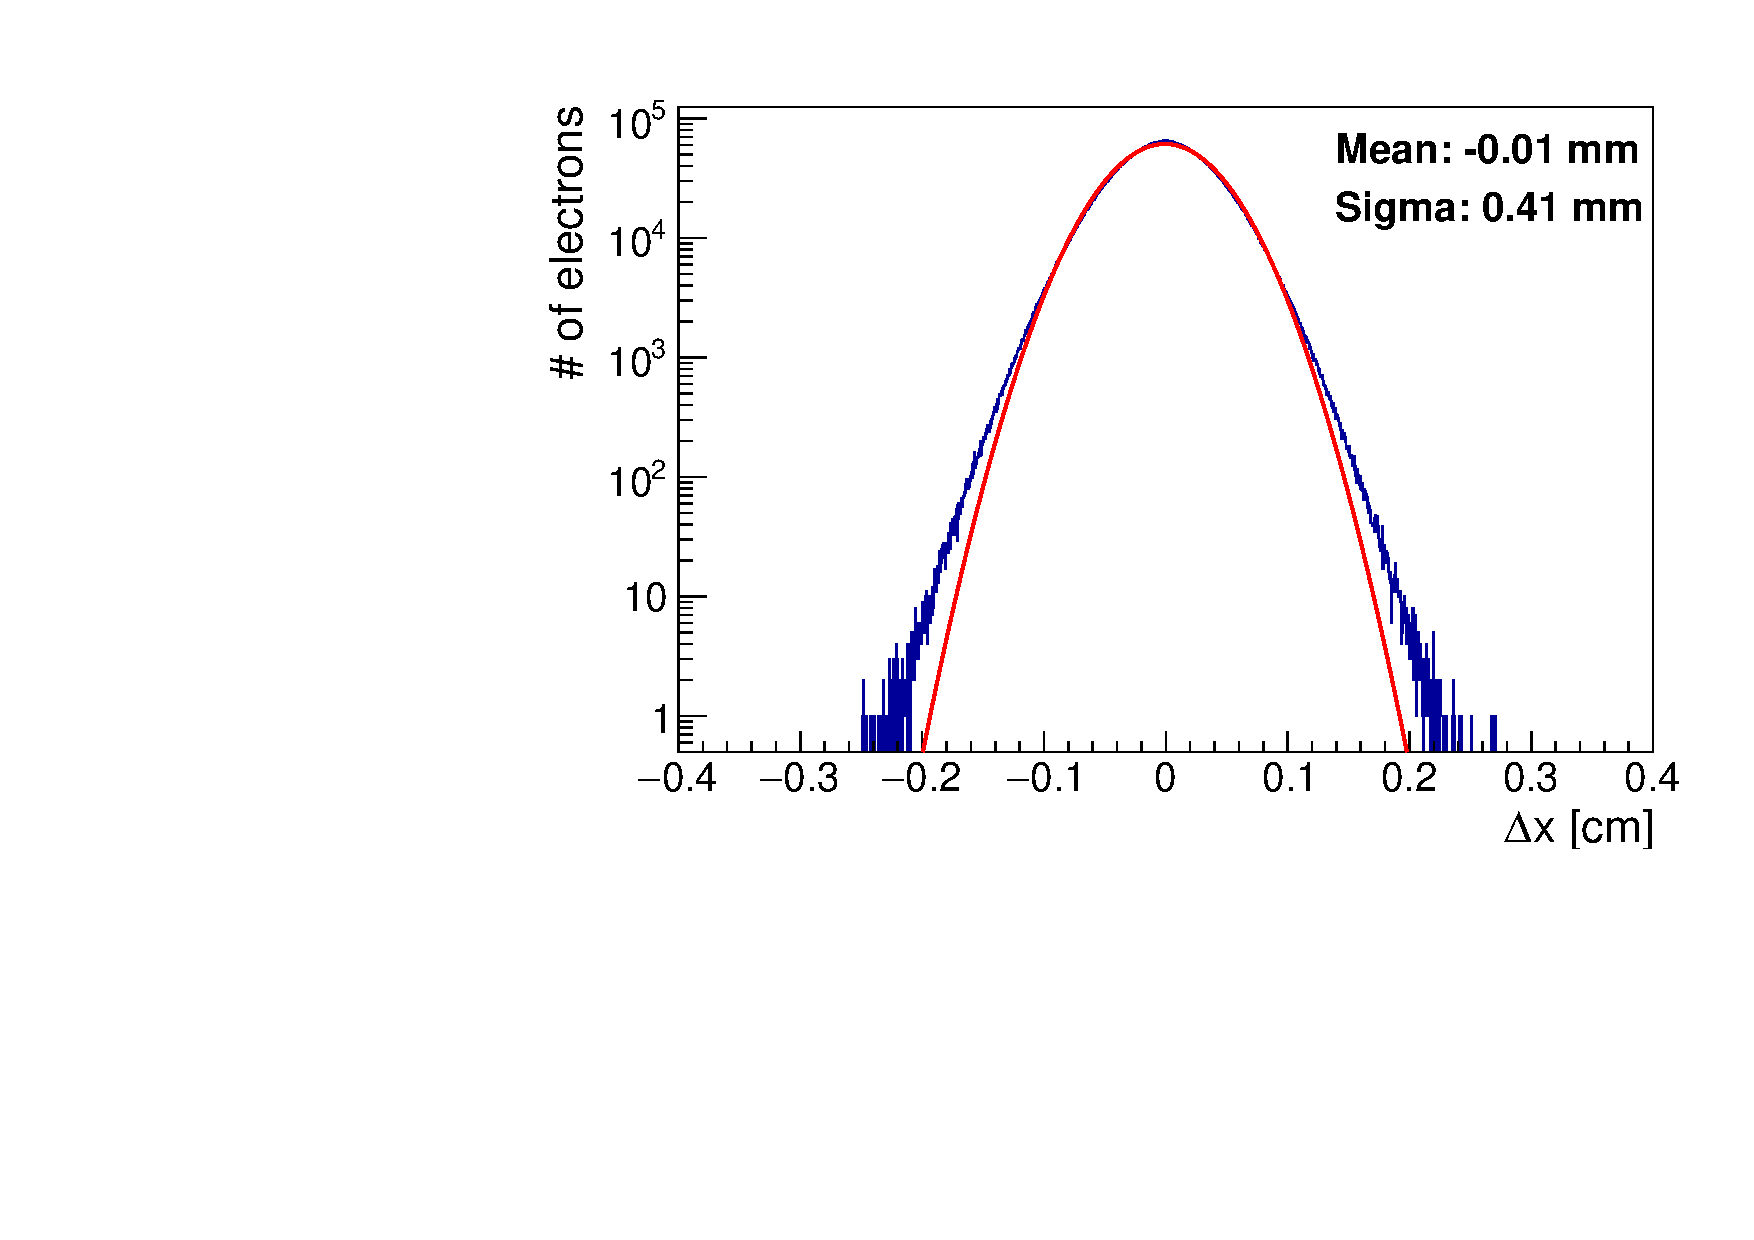
\includegraphics[width=0.45\textwidth]{../../figures/c_fit_res_x_log.pdf}\\
			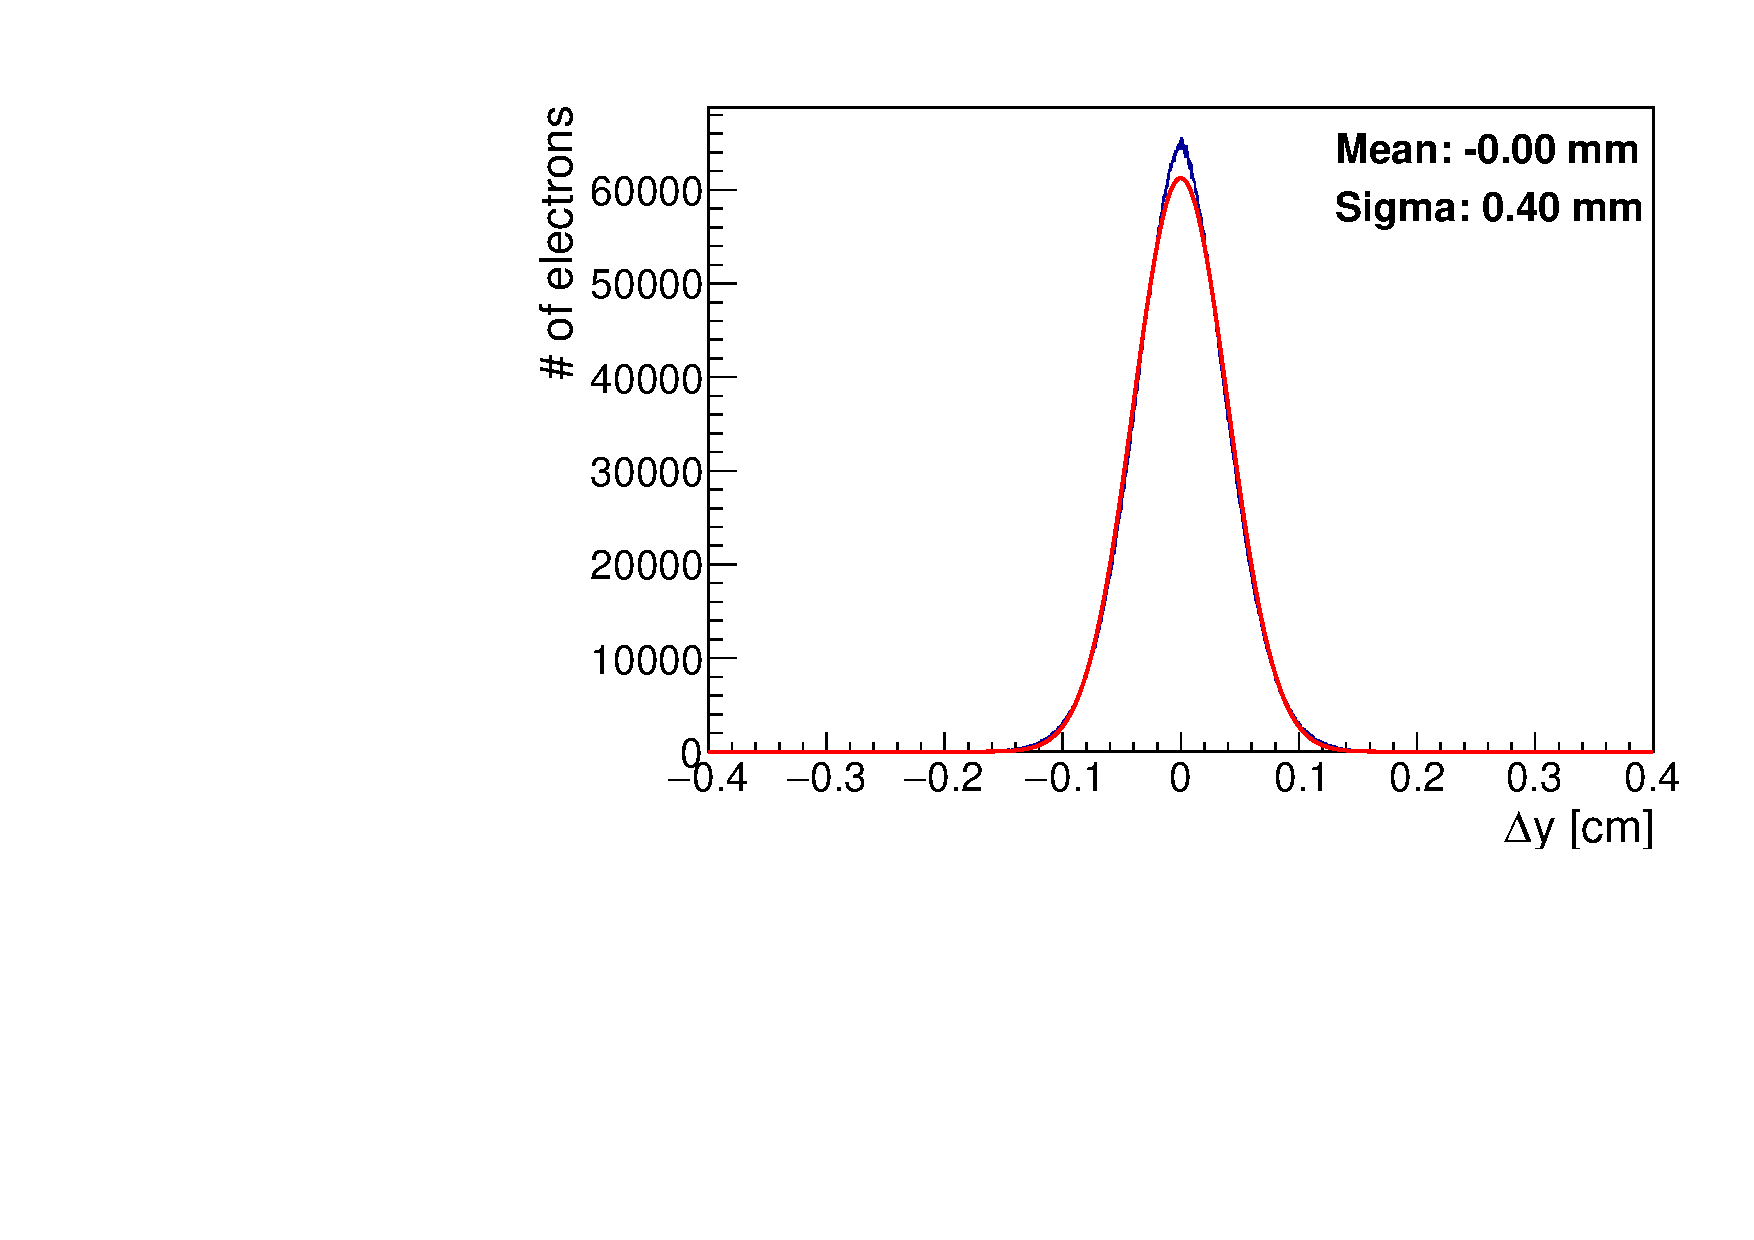
\includegraphics[width=0.45\textwidth]{../../figures/c_fit_res_y_lin.pdf}
			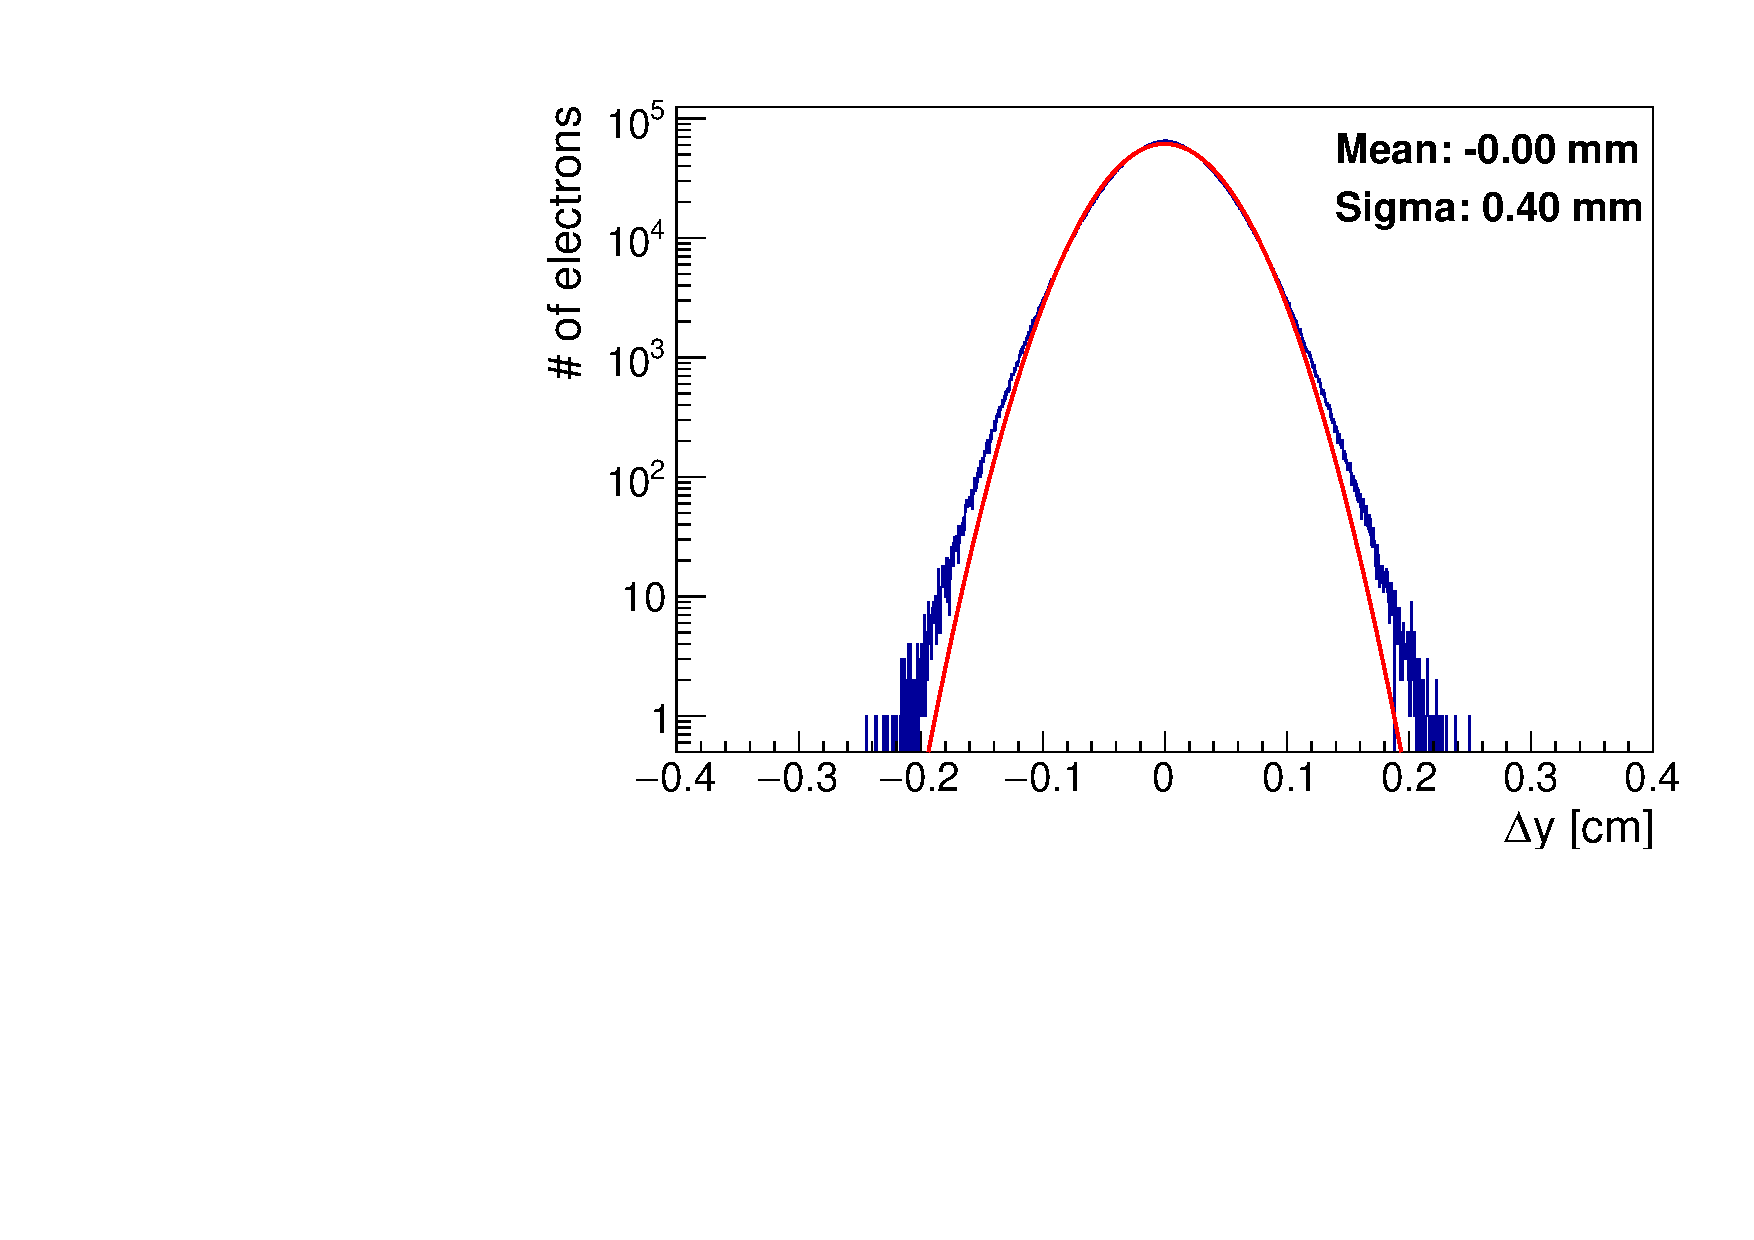
\includegraphics[width=0.45\textwidth]{../../figures/c_fit_res_y_log.pdf}
		\end{frame}
	}
	\begin{frame}
		\frametitle{Ionization Electron Map Reconstruction Residuals ($z$)}
		Residuals of initial positions of 14.3 million simulated track ionization $e^-$ reconstructed using the map\\
		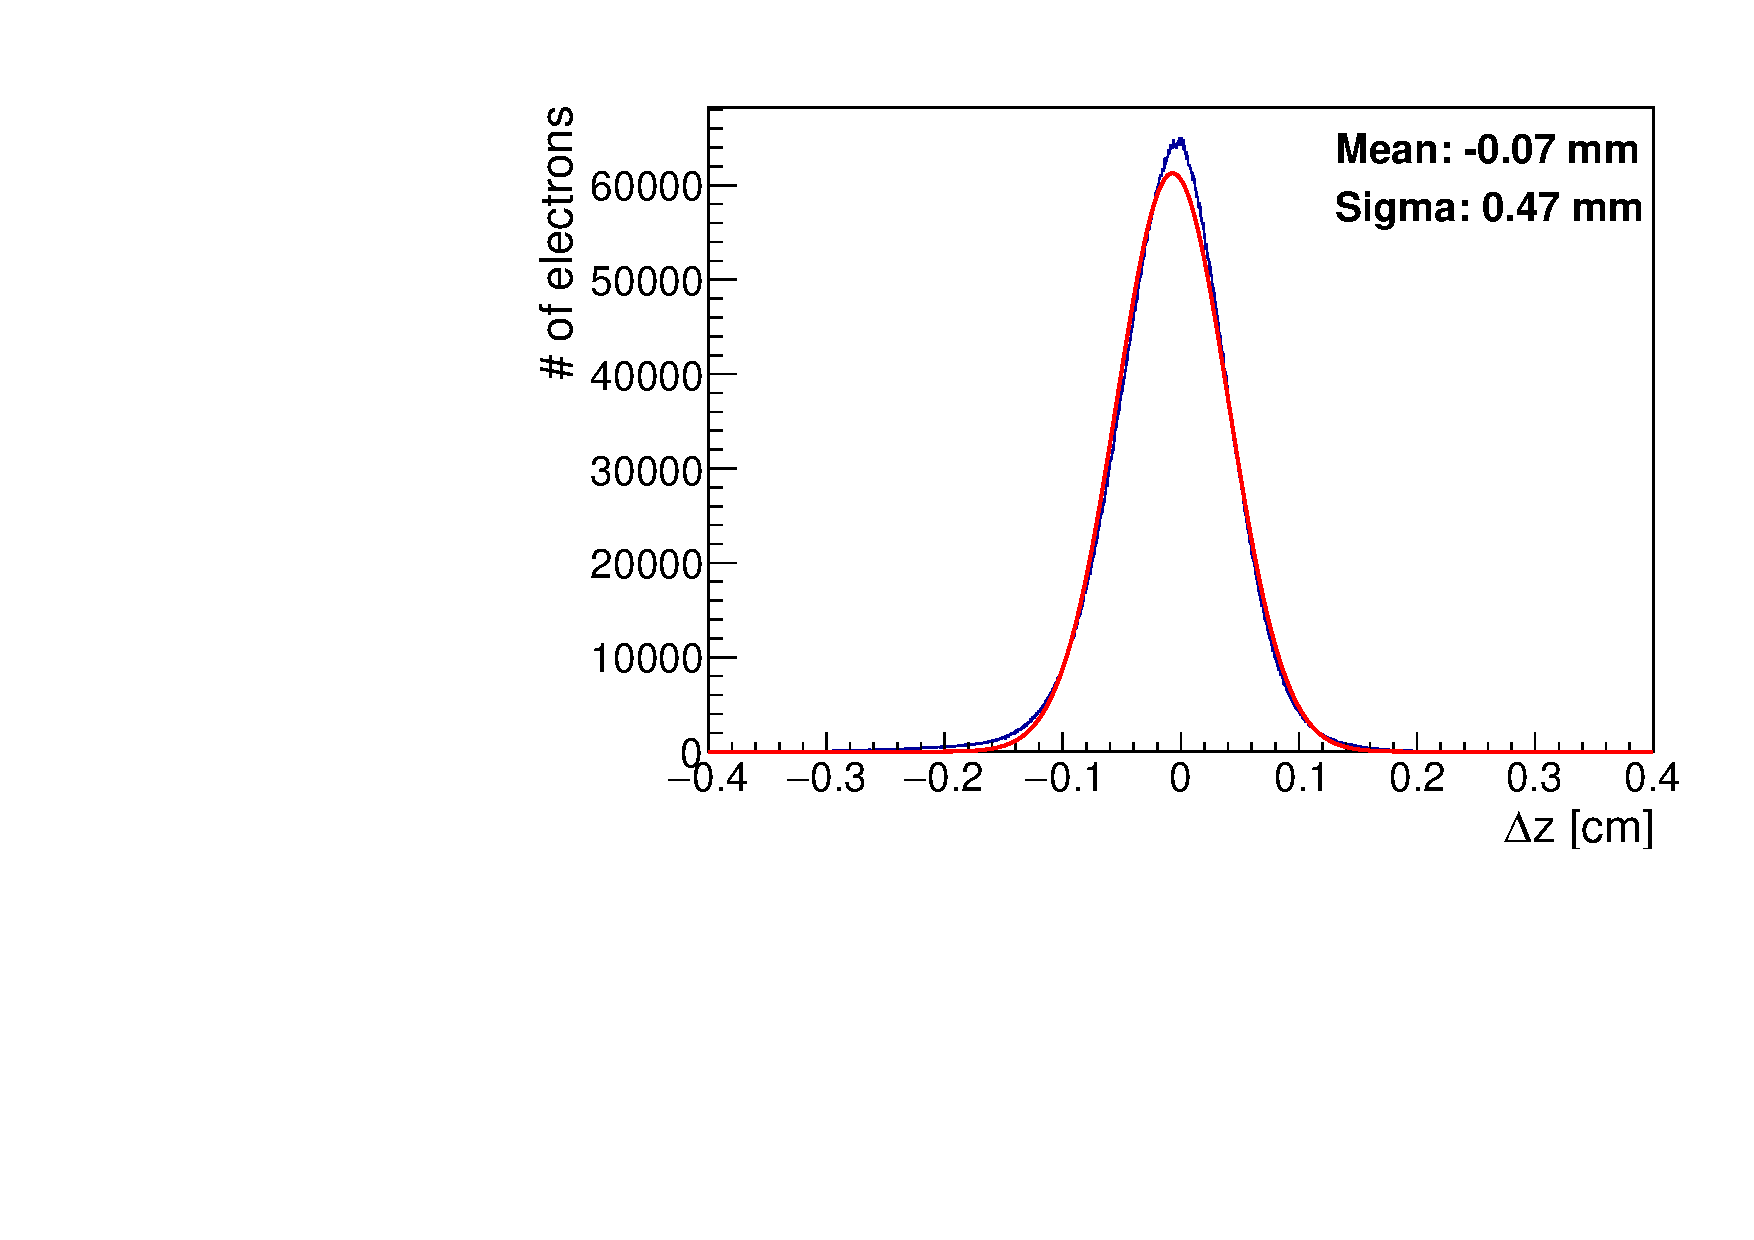
\includegraphics[width=0.45\textwidth]{../../figures/c_fit_res_z_lin.pdf}
		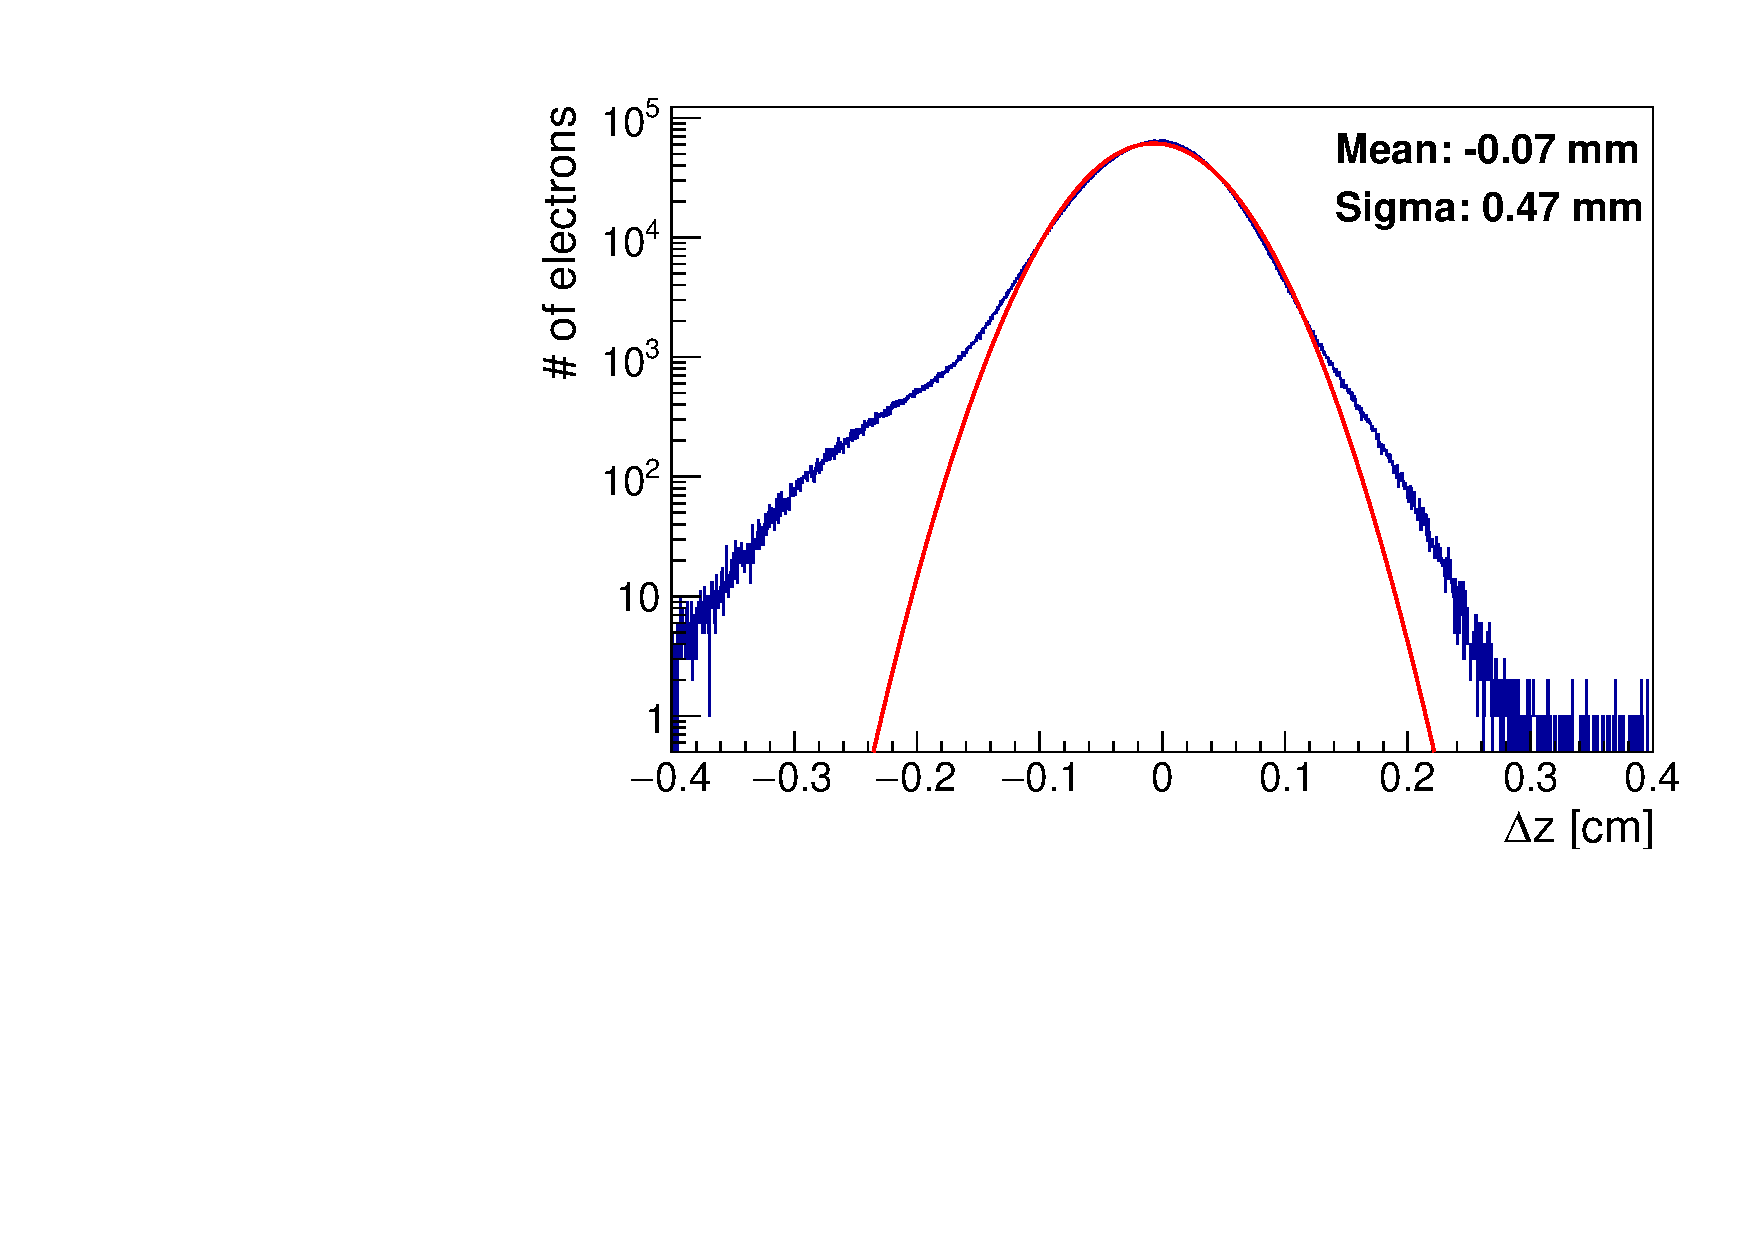
\includegraphics[width=0.45\textwidth]{../../figures/c_fit_res_z_log.pdf}
		Deviations likely caused by non-zero initial velocity of electrons
	\end{frame}
	
	{\nologo\nonav
		\begin{frame}
			\frametitle{Inverse Mapping of Pads}
			
			\begin{tikzpicture}[remember picture,overlay]
				
				% bottom left
				\node[anchor=center] at ([xshift=-3.3cm,yshift=-0.75cm]current page.center)
				{
					\begin{minipage}{0.41\textwidth}
						\centering
						Pad 12 \white{aa} \\
						(near magnet pole) \white{aa}\\ %\vspace{-0.5em}
						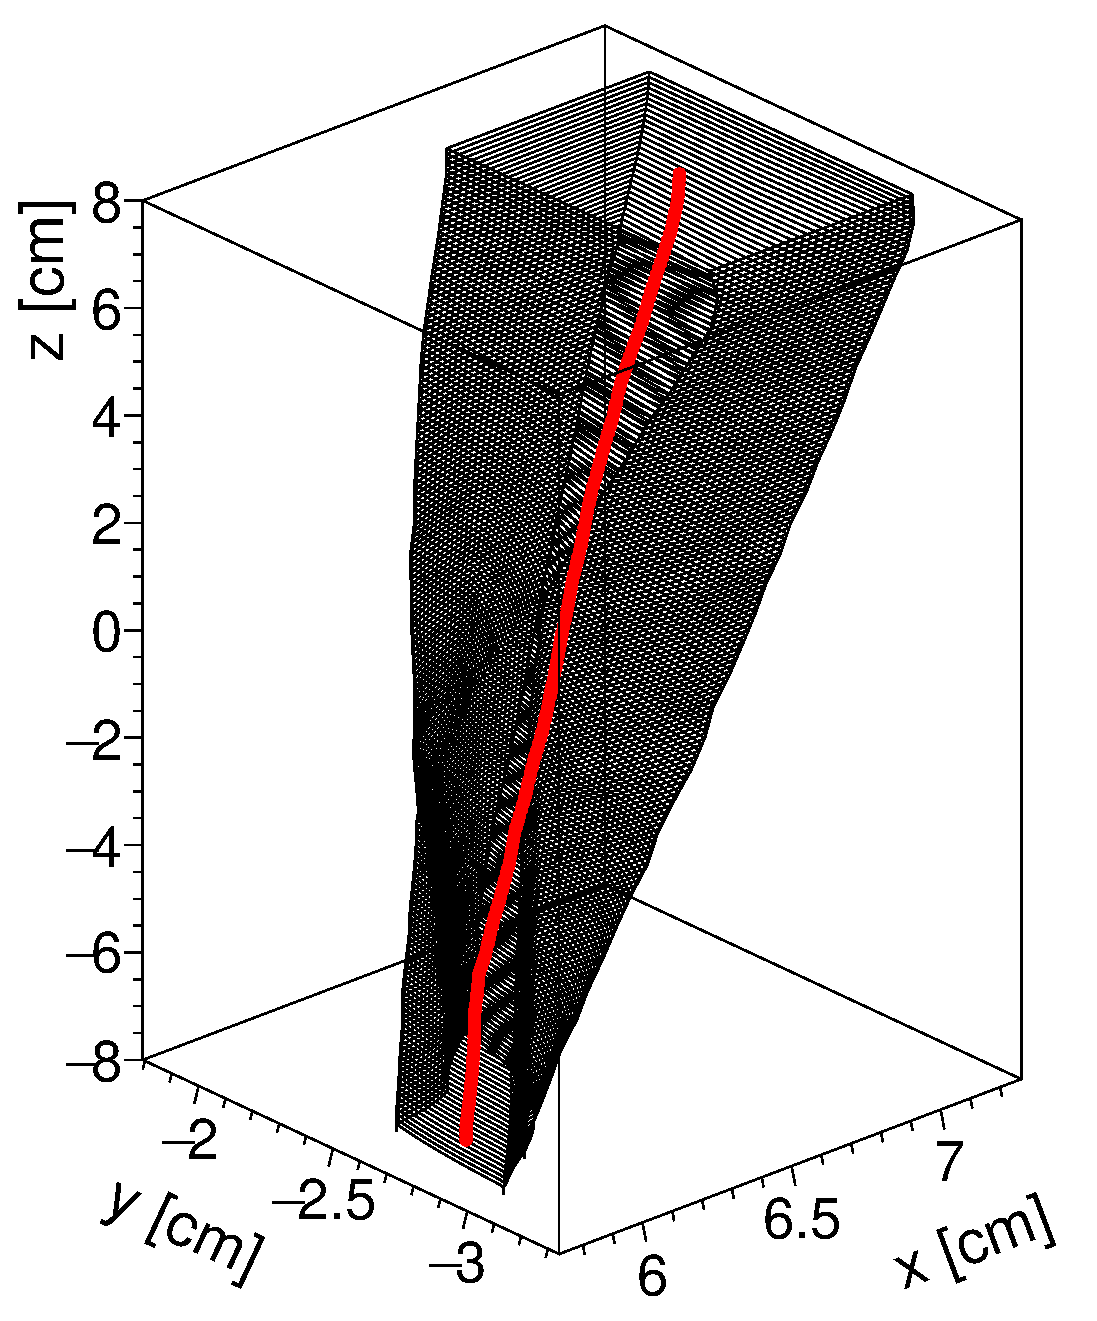
\includegraphics[width=\linewidth]{../../figures/pad_12_grad.pdf}
						\vspace{-1.7em}
						
						Inversion by gradient descent
					\end{minipage}
				};
				
				% bottom right
				\node[anchor=center] at ([xshift=3.3cm,yshift=-0.75cm]current page.center)
				{
					\begin{minipage}{0.41\textwidth}
						\centering
						\white{a} Pad 66\\
						\white{a} (near center)
						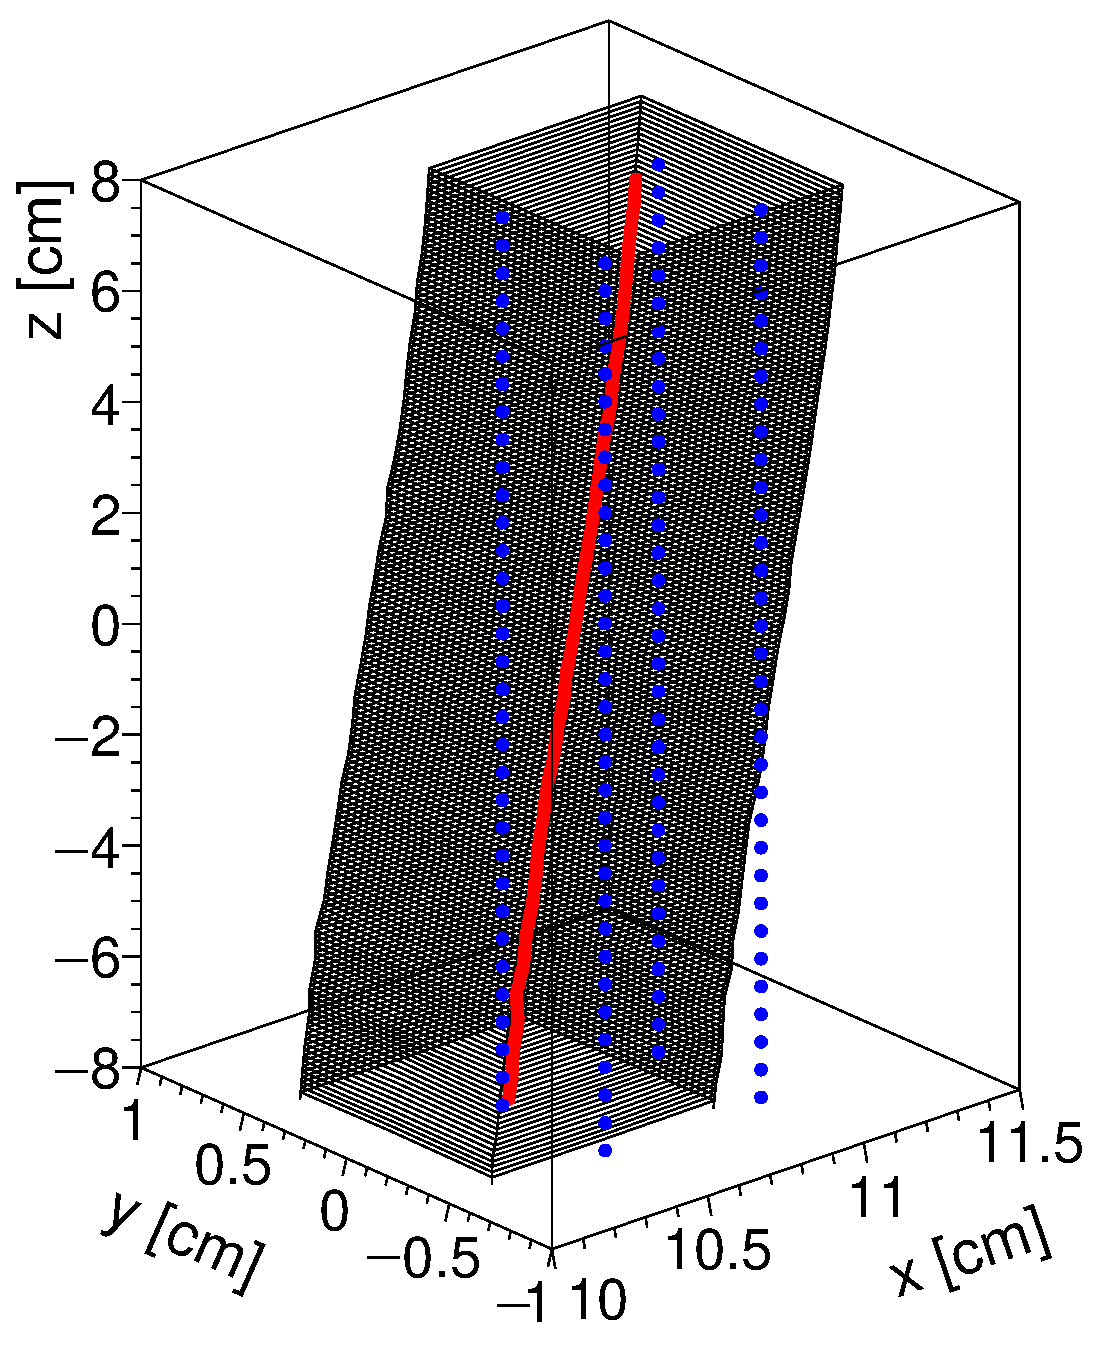
\includegraphics[width=\linewidth]{../../figures/pad_66_interpol.pdf}
						\vspace{-1.7em}
						
						Inversion by interpolation
					\end{minipage}
				};
				
				% top image (drawn LAST → on top)
				\node[anchor=center] at ([yshift=2.65cm]current page.center)
				{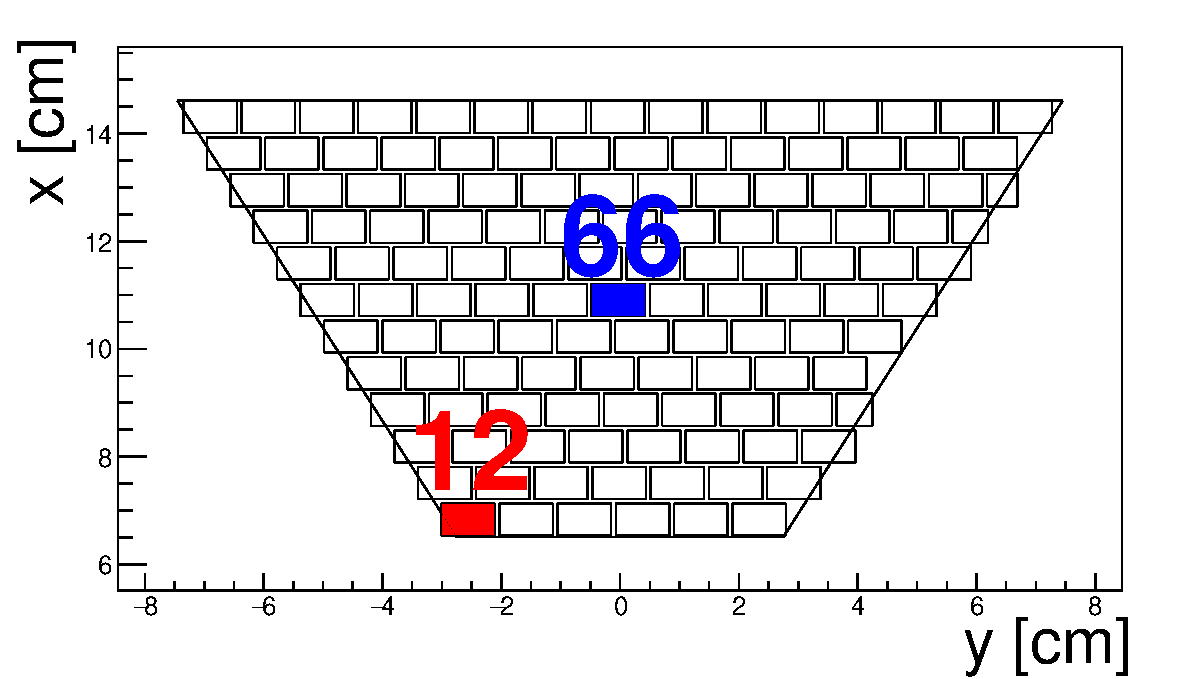
\includegraphics[width=0.33\textwidth]{../../figures/pad_layout_12_66.pdf}};
				
			\end{tikzpicture}
			
		\end{frame}
	}
	
	\begin{frame}
		\frametitle{X17 Decay Signature in IPC (with preliminary errors)}
		\centering
		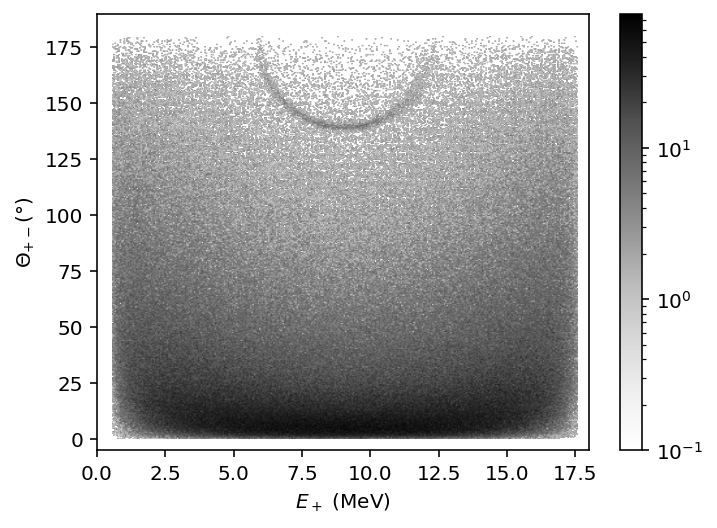
\includegraphics[width=0.75\textwidth]{../images/X17_sim_rand.png}\\
		\vspace{-0.25cm}
		\begin{minipage}[t][4cm]{0.85\textwidth}
			\textbf{Geant 4 simulation + errors:} Histogram of e$^+$e$^-$ pair angle and positron energy produced by standard IPC and by the decay of a hypothetical boson X17 (branching ratio $3\cdot10^{-3}$).
		\end{minipage}
	\end{frame}
	\begin{frame}
		\frametitle{Reconstruction Testing Summary}
		\begin{enumerate}
			\item Ionization electron map simulation of ionization electrons in the entire volume of the OFTPC
			\item Track(s) simulated using HEED and microscopic tracking
			\item Counting the number of ionization $e^-$ in each pad and time bin of the readout
			\item Using the map to reconstruct the position of centers of pads for given centers of time bins
			\item Fitting of the reconstructed points with circle and lines fit using least squares weighted by the number of ionization $e^-$ in each point
			\item Using the magnetic field in the middle of the track to get first energy estimate
			\item Using the 4\textsuperscript{th} order Runge-Kutta fit with least squares to refine the energy estimate
			\item Correct systematic errors using a 3 parameter linear function
		\end{enumerate}
	\end{frame}
	{\nologo\nonav
	\begin{frame}
		\frametitle{Runge-Kutta energy comparison}
		\centering
		\includegraphics[width=0.57\textwidth]{figures/rk_forward.png}\\
		\vspace{-0.2cm}
		\small{Comparison of 25 tracks with same initial position and orientation and different energies in the range 3--13~MeV.}
	\end{frame}
	}
	\begin{frame}
		\frametitle{Magnetic field in the XZ plane}
		\centering
		\includegraphics[width=0.6\textwidth]{figures/mag_xz.png}
	\end{frame}
	
	\begin{frame}
		\frametitle{Energy Reconstruction Precision (energy dependence)}
		\centering
		\begin{columns}
			\column{0.5\textwidth}
			\centering
			\Large \textbf{Electrons}
			\begin{figure}
				\centering
				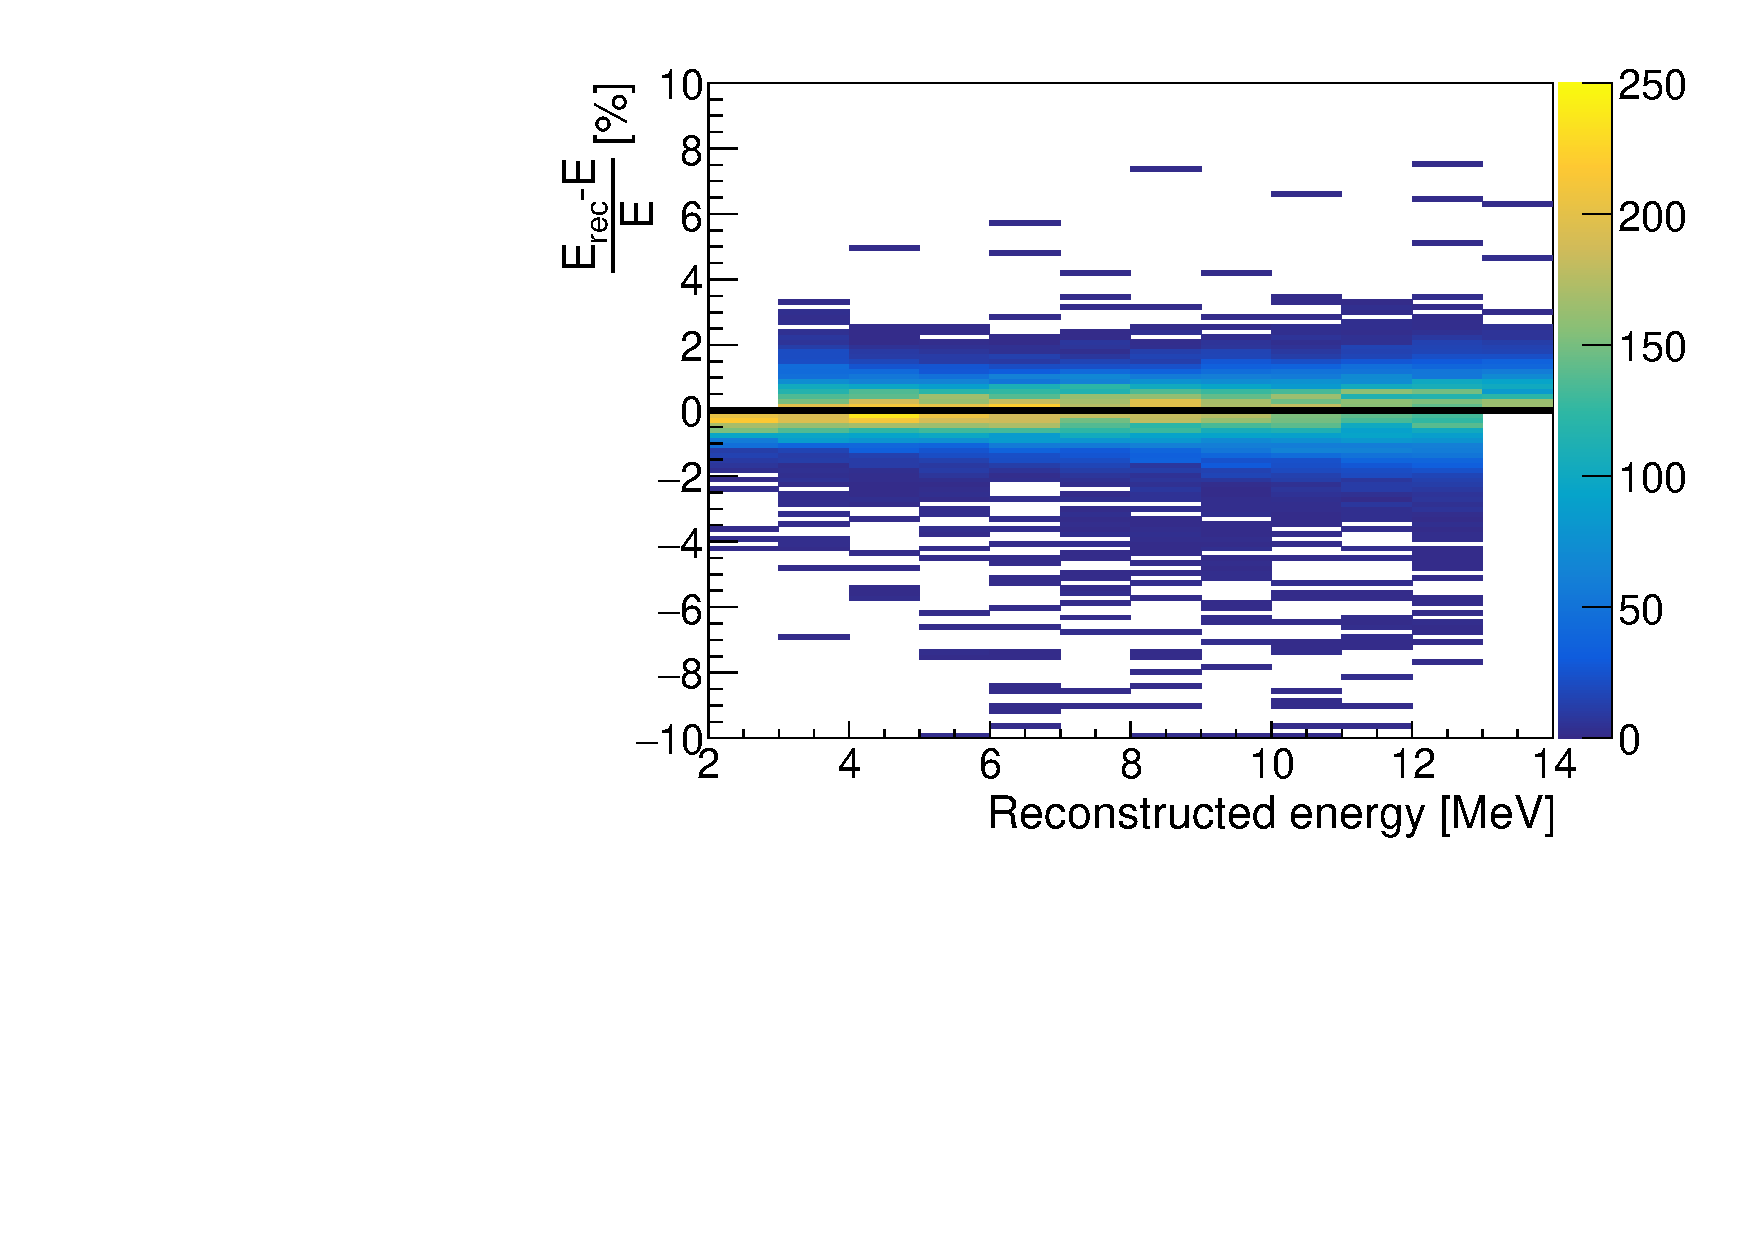
\includegraphics[width = 0.95 \linewidth]{../../figures/c_e_deltaenergy_energy2.pdf}
			\end{figure}
			\column{0.5\textwidth}
			\centering
			\Large \textbf{Positrons}
			\begin{figure}
				\centering
				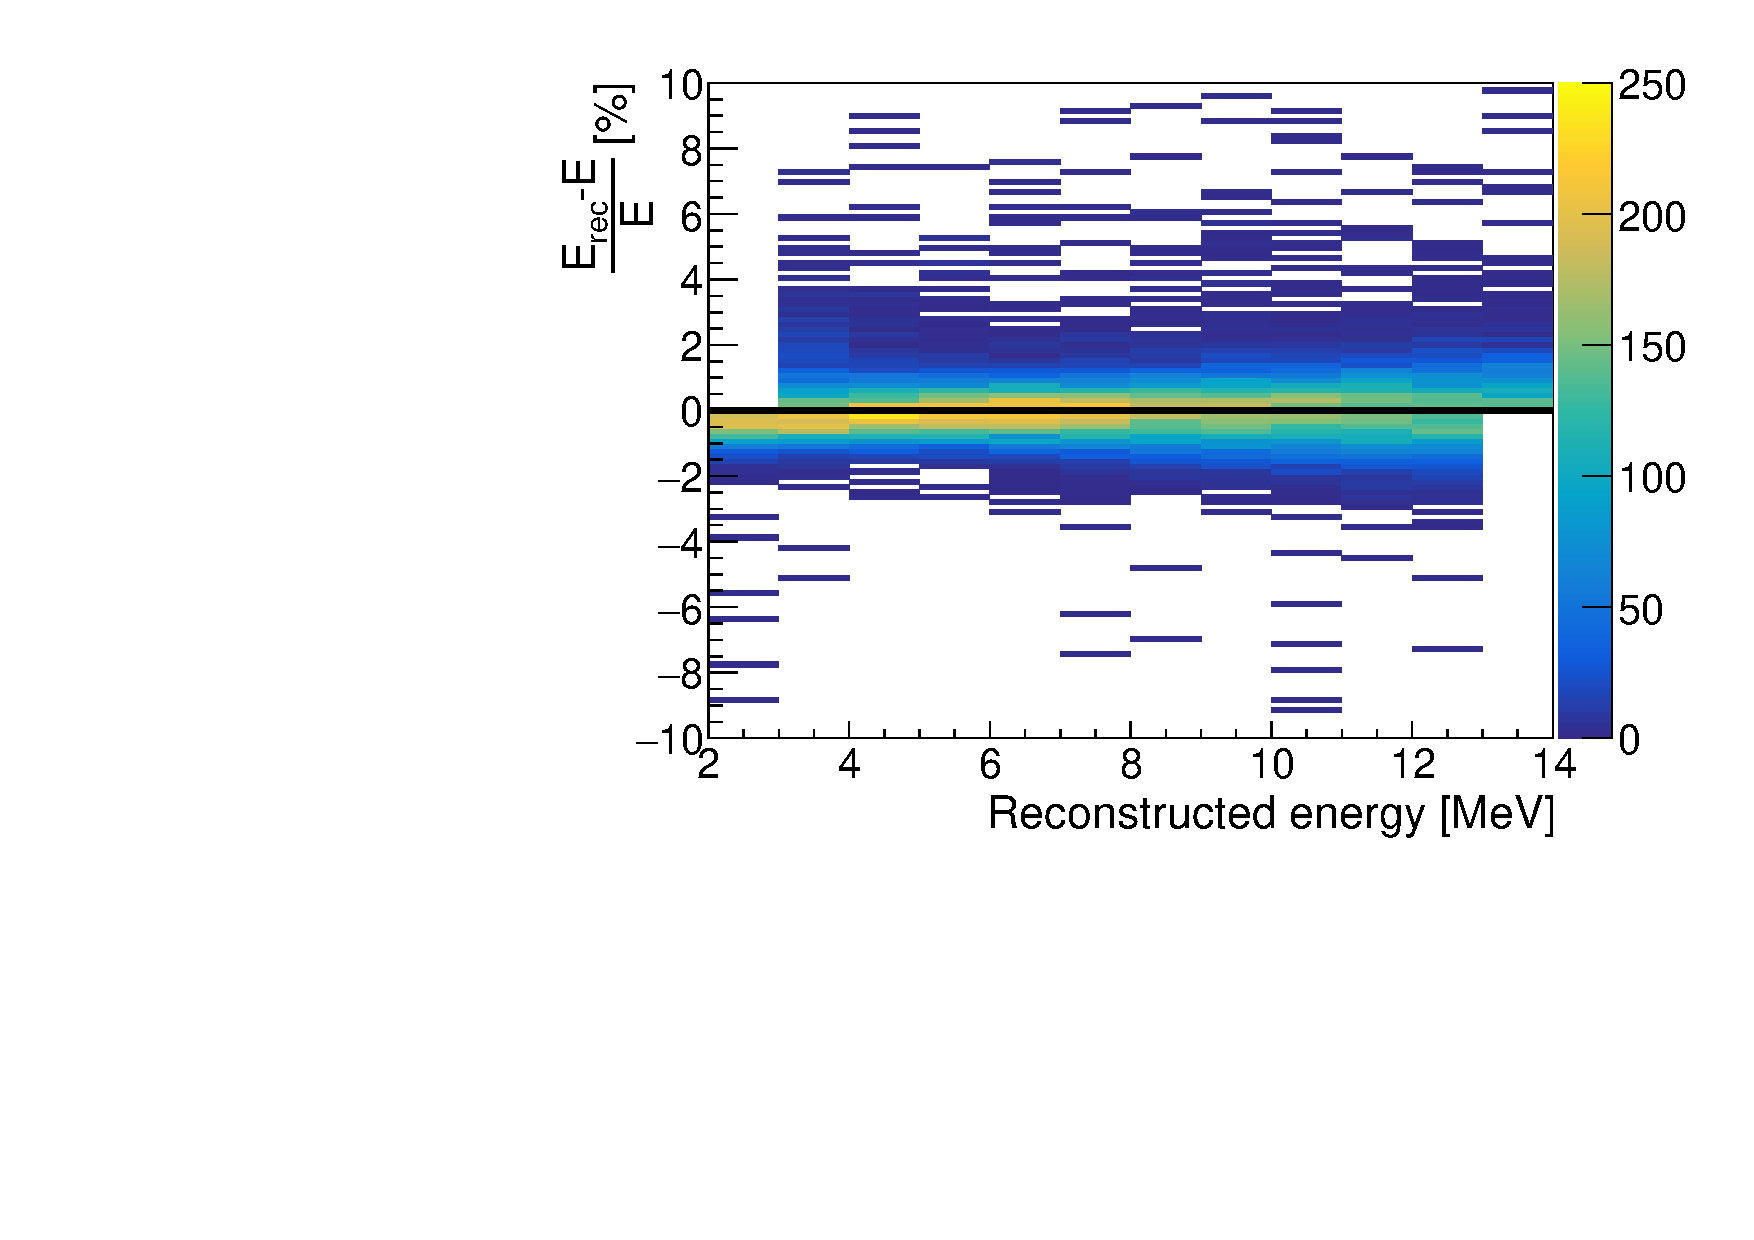
\includegraphics[width = 0.95 \linewidth]{../../figures/c_p_deltaenergy_energy2.pdf}
			\end{figure}
		\end{columns}
		\vspace{0.5cm}
		\footnotesize{Relative reconstruction deviation of the~kinetic energy of electron and positron tracks (ca. 24\,000 of each simulated).}
	\end{frame}
	\begin{frame}
		\frametitle{Energy Reconstruction Precision (theta dependence)}
		\centering
		\begin{columns}
			\column{0.5\textwidth}
			\centering
			\Large \textbf{Electrons}
			\begin{figure}
				\centering
				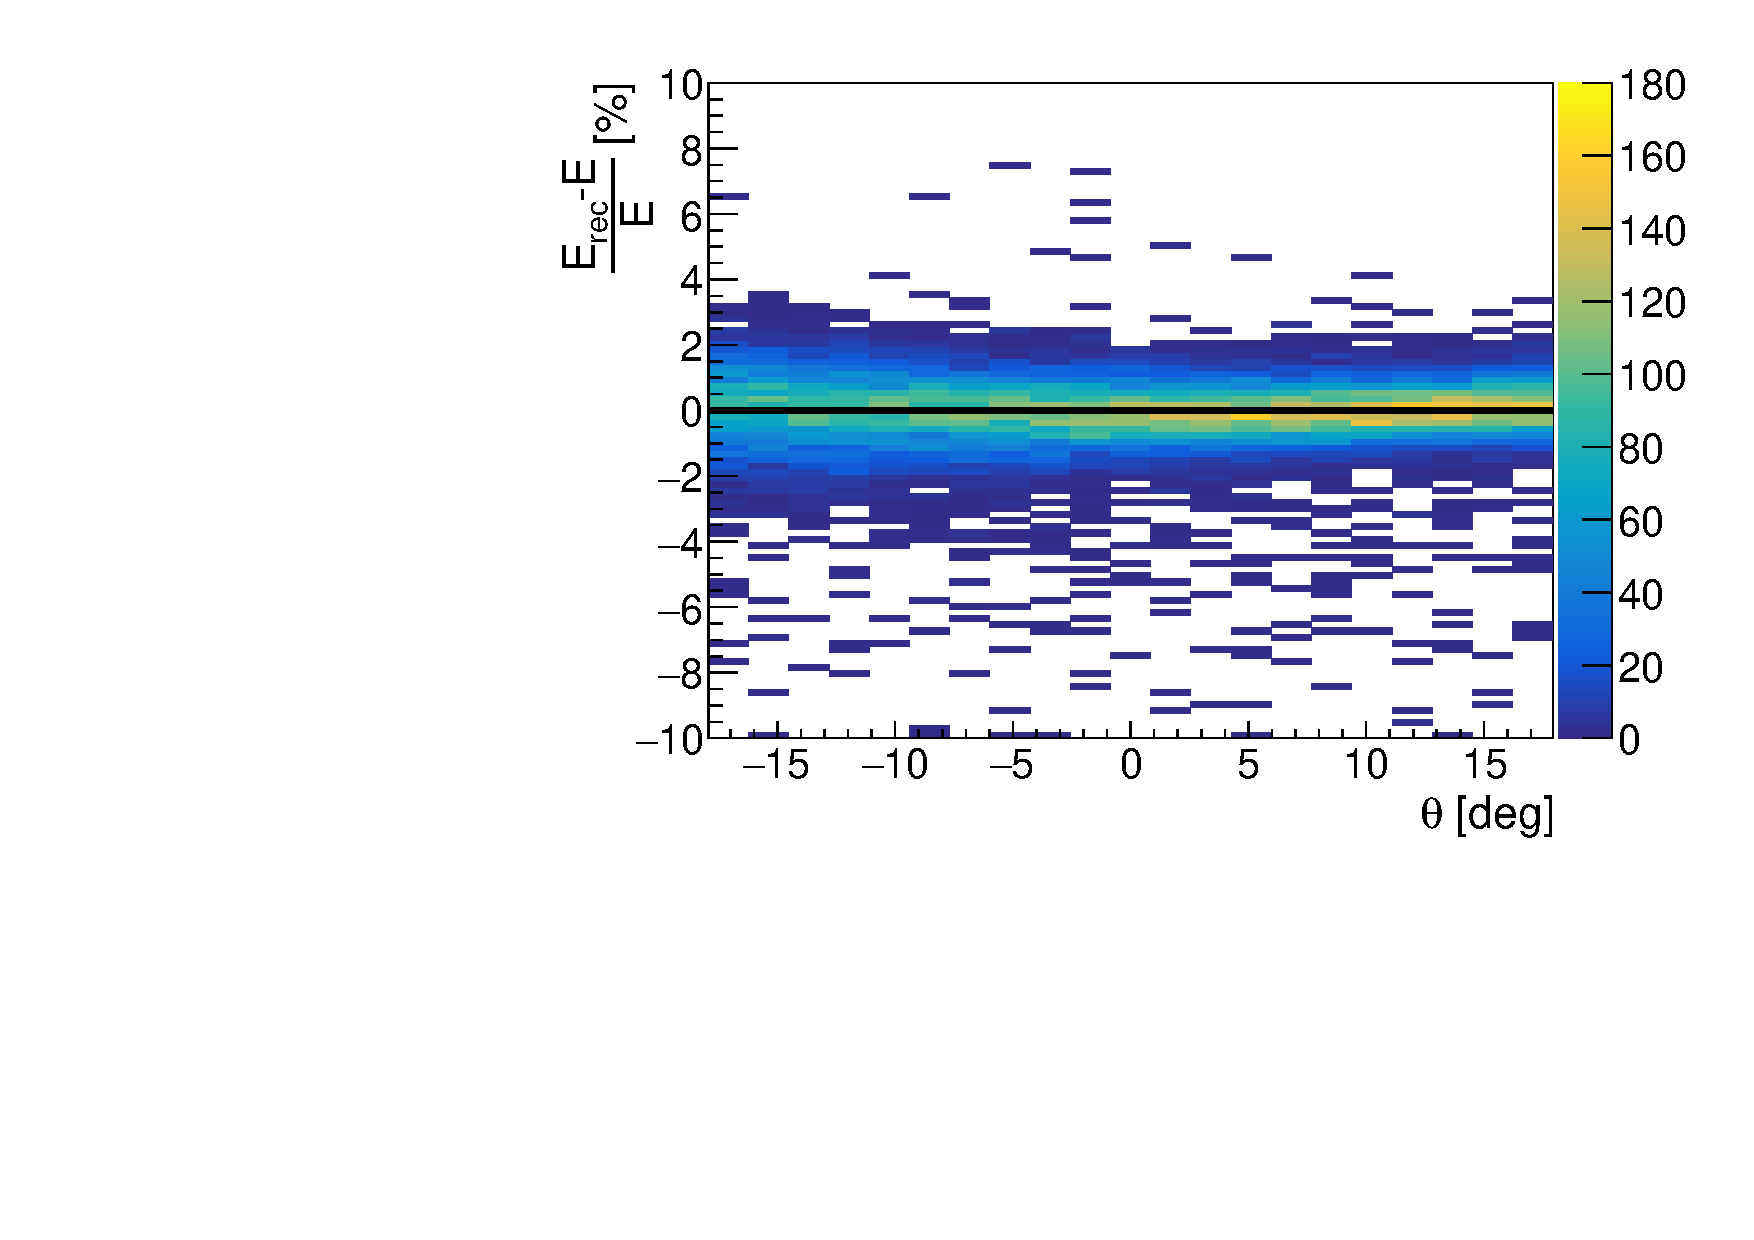
\includegraphics[width = 0.95 \linewidth]{../../figures/c_e_deltaenergy_theta.pdf}
			\end{figure}
			\column{0.5\textwidth}
			\centering
			\Large \textbf{Positrons}
			\begin{figure}
				\centering
				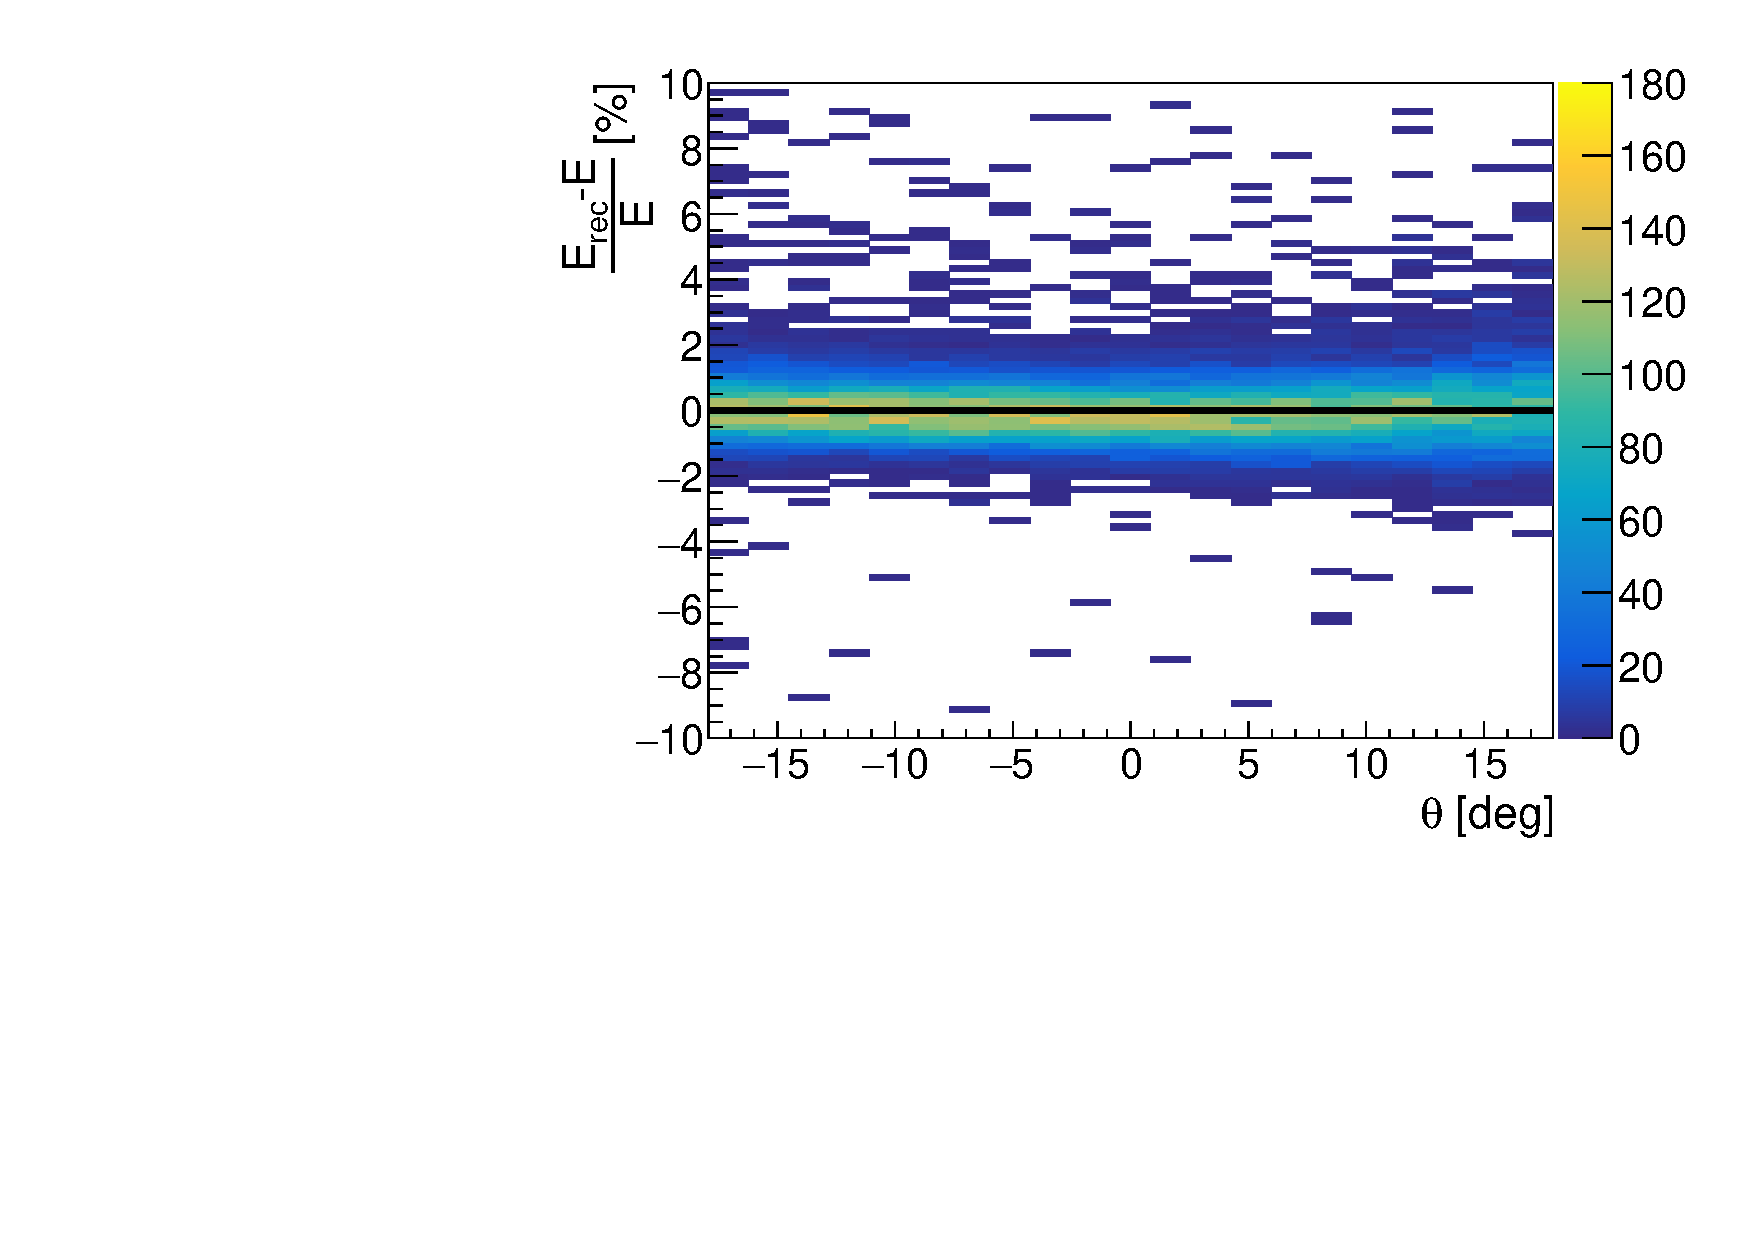
\includegraphics[width = 0.95 \linewidth]{../../figures/c_p_deltaenergy_theta.pdf}
			\end{figure}
		\end{columns}
		\vspace{0.5cm}
		\footnotesize{Relative reconstruction deviation of the~kinetic energy of electron and positron tracks (ca. 24\,000 of each simulated).}
	\end{frame}
	\begin{frame}
		\frametitle{Energy Reconstruction Precision (phi dependence)}
		\centering
		\begin{columns}
			\column{0.5\textwidth}
			\centering
			\Large \textbf{Electrons}
			\begin{figure}
				\centering
				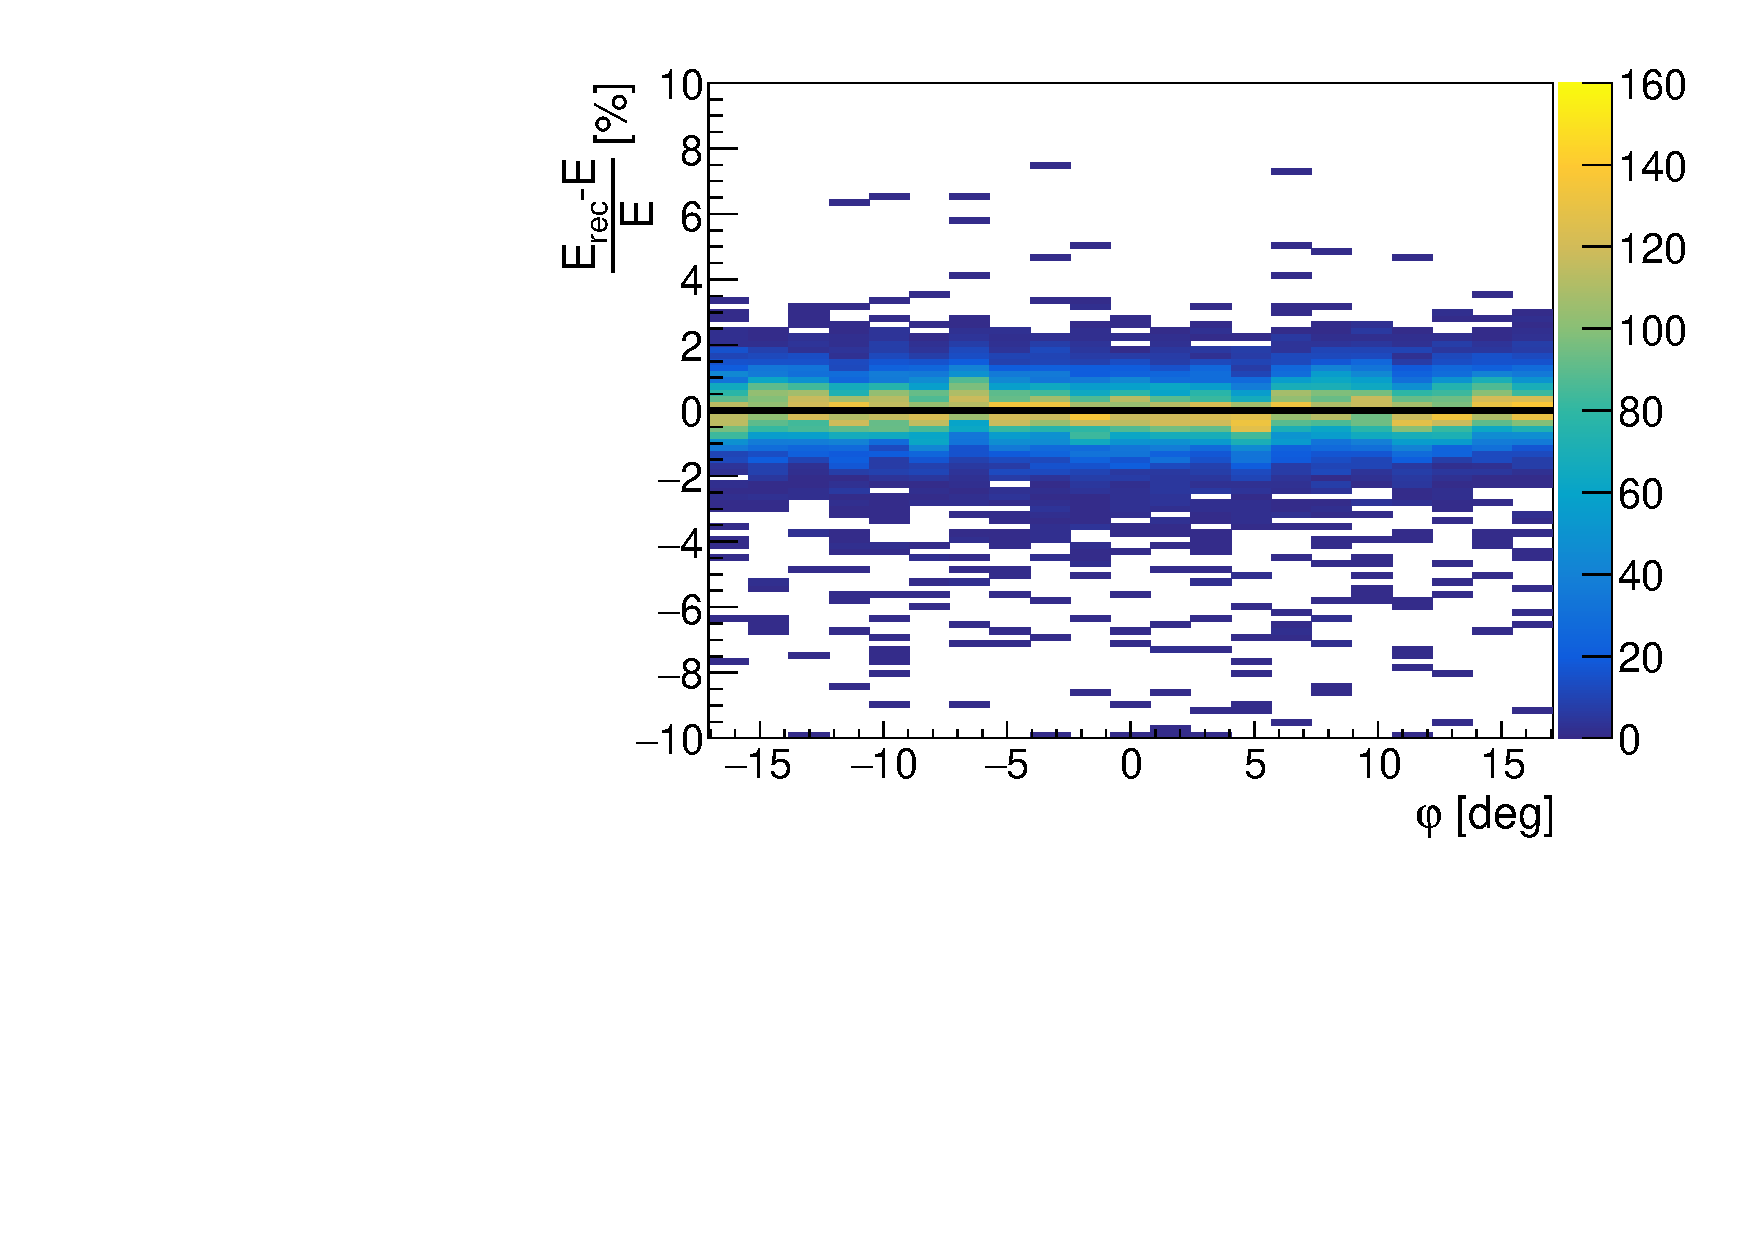
\includegraphics[width = 0.95 \linewidth]{../../figures/c_e_deltaenergy_phi.pdf}
			\end{figure}
			\column{0.5\textwidth}
			\centering
			\Large \textbf{Positrons}
			\begin{figure}
				\centering
				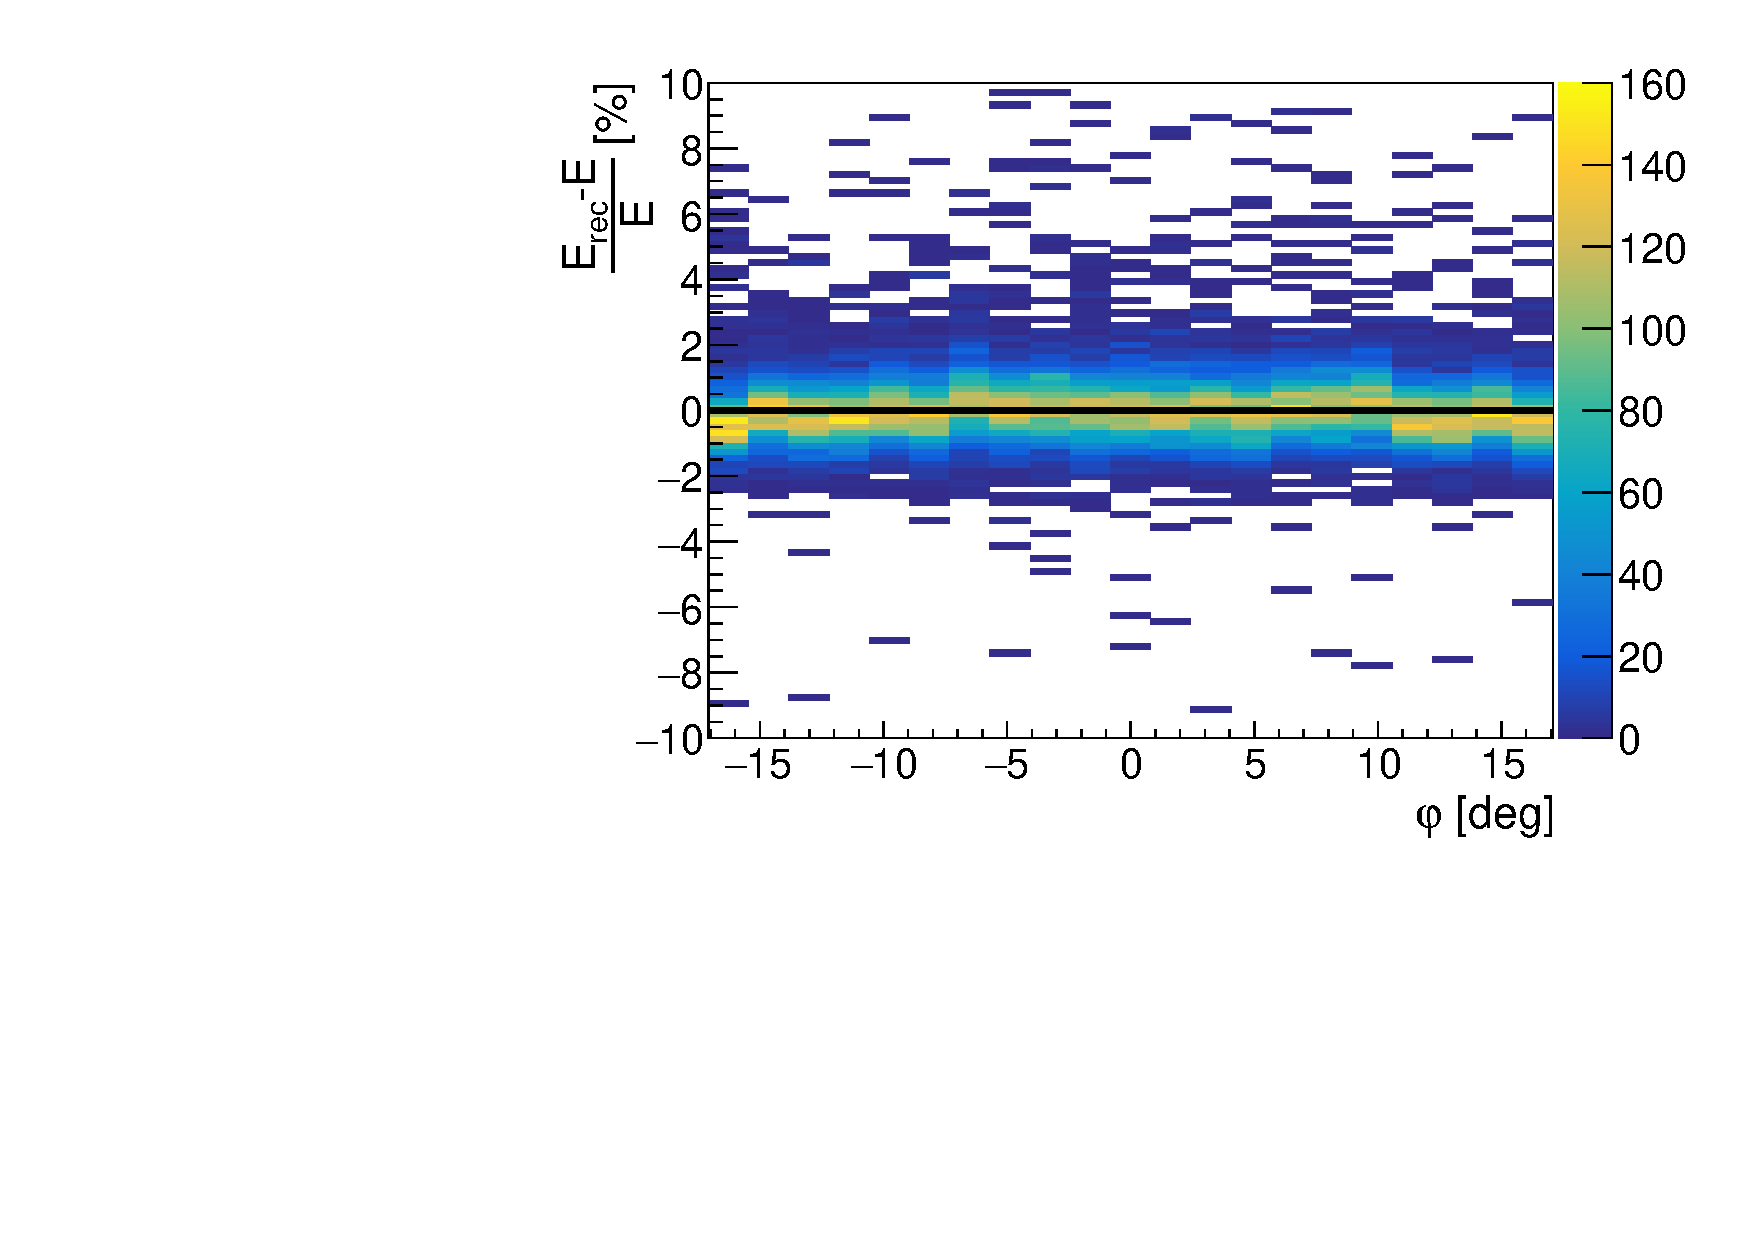
\includegraphics[width = 0.95 \linewidth]{../../figures/c_p_deltaenergy_phi.pdf}
			\end{figure}
		\end{columns}
		\vspace{0.5cm}
		\footnotesize{Relative reconstruction deviation of the~kinetic energy of electron and positron tracks (ca. 24\,000 of each simulated).}
	\end{frame}
	\begin{frame}
		\frametitle{Future Steps}
		\begin{itemize}
			\item Complete the Geant4 simulation with multiple scattering for the full parameter grid
			\item Account for parasitic tracks caused by high energy secondary electrons
			\item Account for GEM in the simulation, charge distribution between pads
			\item Account for noise (denoising using a convolutional neural network --- M. Gajdoš~\cite{Gajdoš_2025})
			\item Optimize Runge-Kutta integration fit with likelihood approach (instead of least squares) if needed
			\item Test different geometries
			\item Make a better simulation of magnetic and electric fields, compare with measurements
		\end{itemize}
	\end{frame}
\end{document}